%% abtex2-modelo-trabalho-academico.tex, v<VERSION> laurocesar
%% Copyright 2012-2015 by abnTeX2 group at http://www.abntex.net.br/ 
%%
%% This work may be distributed and/or modified under the
%% conditions of the LaTeX Project Public License, either version 1.3
%% of this license or (at your option) any later version.
%% The latest version of this license is in
%%   http://www.latex-project.org/lppl.txt
%% and version 1.3 or later is part of all distributions of LaTeX
%% version 2005/12/01 or later.
%%
%% This work has the LPPL maintenance status `maintained'.
%% 
%% The Current Maintainer of this work is the abnTeX2 team, led
%% by Lauro César Araujo. Further information are available on 
%% http://www.abntex.net.br/
%%
%% This work consists of the files abntex2-modelo-trabalho-academico.tex,
%% abntex2-modelo-include-comandos and abntex2-modelo-references.bib
%%

% ------------------------------------------------------------------------
% ------------------------------------------------------------------------
% abnTeX2: Modelo de Trabalho Academico (tese de doutorado, dissertacao de
% mestrado e trabalhos monograficos em geral) em conformidade com 
% ABNT NBR 14724:2011: Informacao e documentacao - Trabalhos academicos -
% Apresentacao
% ------------------------------------------------------------------------
% ------------------------------------------------------------------------

\documentclass[
	% -- opções da classe memoir --
	12pt,				% tamanho da fonte
	openright,			% capítulos começam em pág ímpar (insere página vazia caso preciso)
	%twoside,			% para impressão em verso e anverso. Oposto a oneside
  oneside,     % para impressão em verso e anverso. Oposto a twoside
	a4paper,			% tamanho do papel. 
	% -- opções da classe abntex2 --
	%chapter=TITLE,		% títulos de capítulos convertidos em letras maiúsculas
	%section=TITLE,		% títulos de seções convertidos em letras maiúsculas
	%subsection=TITLE,	% títulos de subseções convertidos em letras maiúsculas
	%subsubsection=TITLE,% títulos de subsubseções convertidos em letras maiúsculas
	% -- opções do pacote babel --
	% english,			% idioma adicional para hifenização
	% french,				% idioma adicional para hifenização
	% spanish,			% idioma adicional para hifenização
	brazil				% o último idioma é o principal do documento
	]{abntex2}

  \renewcommand{\ABNTEXchapterfont}{\bfseries}
  \renewcommand{\ABNTEXchapterfontsize}{\normalsize}
  \renewcommand{\ABNTEXsectionfont}{\bfseries}
  \renewcommand{\ABNTEXsectionfontsize}{\normalsize}
  \renewcommand{\ABNTEXsubsectionfont}
  \renewcommand{\ABNTEXsubsectionfontsize}{\normalsize}

  \usepackage{booktabs}
  % \usepackage{caption}
  % \captionsetup[table]{name=Quadro}

  \addto\captionsbrazil{%
  \renewcommand{\tablename}{Quadro}
  \renewcommand{\listtablename}{Lista de quadros}
  }

  \usepackage{multirow}
  \usepackage{enumitem}
  \SetEnumitemKey{midsep}{itemsep=0pt, parsep=0pt}

  % \usepackage[capposition=top]{floatrow}
% ---
% Pacotes básicos 
% ---
% \usepackage{helvet}
% \renewcommand{\familydefault}{\sfdefault}
% \usepackage{lmodern}			% Usa a fonte Latin Modern
% \usepackage{cfr-lm}      % Technically, lmodern does since the fonts it installs are identical to those used by cfr-lm		
\usepackage[T1]{fontenc}		% Selecao de codigos de fonte.
\usepackage[utf8]{inputenc}		% Codificacao do documento (conversão automática dos acentos)
\usepackage{lastpage}			% Usado pela Ficha catalográfica
\usepackage{indentfirst}		% Indenta o primeiro parágrafo de cada seção.
\usepackage{color}				% Controle das cores
\usepackage{graphicx}			% Inclusão de gráficos
\usepackage{microtype} 			% para melhorias de justificação

%%%%%%%%%%%%%%%%%%%%%%
% pacotes incluídos
\usepackage{longtable}
\usepackage{lscape}
\usepackage{supertabular}
\usepackage[small]{caption}
\usepackage[toc,acronym]{glossaries}
\usepackage[toc]{glossaries}

%\usepackage{fontspec}
%\usepackage{fontawesome}
\usepackage{hyperref}
%%%%%%%%%%%%%%%%%%%%%%
% ---
		
% ---
% Pacotes adicionais, usados apenas no âmbito do Modelo Canônico do abnteX2
% ---
\usepackage{lipsum}				% para geração de dummy text
% ---

% ---
% Pacotes de citações
% ---
\usepackage[brazilian,hyperpageref]{backref}	 % Paginas com as citações na bibl
\usepackage[alf]{abntex2cite}	% Citações padrão ABNT

% --- 
% CONFIGURAÇÕES DE PACOTES
% --- 

% ---
% Configurações do pacote backref
% Usado sem a opção hyperpageref de backref
\renewcommand{\backrefpagesname}{Citado na(s) página(s):~}
% Texto padrão antes do número das páginas
\renewcommand{\backref}{}
% Define os textos da citação
\renewcommand*{\backrefalt}[4]{
	\ifcase #1 %
		Nenhuma citação no texto.%
	\or
		Citado na página #2.%
	\else
		Citado #1 vezes nas páginas #2.%
	\fi}%
% ---

% ---
% Configurações de aparência do PDF final

% alterando o aspecto da cor azul
\definecolor{blue}{RGB}{41,5,195}

% definindo comandos para fontawesome

% \newfontfamily{\FA}{FontAwesome Regular}
% \def\twitter{{\FA \faTwitter}}


% informações do PDF
\makeatletter
\hypersetup{
     	%pagebackref=true,
		pdftitle={\@title}, 
		pdfauthor={\@author},
    	pdfsubject={\imprimirpreambulo},
	    pdfcreator={LaTeX with abnTeX2},
		pdfkeywords={abnt}{latex}{abntex}{abntex2}{trabalho acadêmico}, 
		colorlinks=true,       		% false: boxed links; true: colored links
    	linkcolor=blue,          	% color of internal links
    	citecolor=blue,        		% color of links to bibliography
    	filecolor=magenta,      		% color of file links
		urlcolor=blue,
		bookmarksdepth=4
}
\makeatother
% --- 

% --- 
% Espaçamentos entre linhas e parágrafos 
% --- 

% O tamanho do parágrafo é dado por:
\setlength{\parindent}{1.3cm}

% Controle do espaçamento entre um parágrafo e outro:
\setlength{\parskip}{0.2cm}  % tente também \onelineskip

% ---
% compila o indice
% ---
\makeindex
% ---

\makeglossaries

\newacronym{abenge}{ABENGE}{Associação Brasileira de Educação em Engenharia}
\newacronym{abnt}{ABNT}{Associação Brasileira de Normas Técnicas}
\newacronym{acei}{ACEI}{Assessoria de Cooperação Internacional}
\newacronym{acg}{ACG}{Avaliação dos Cursos de Graduação}
\newacronym{aee}{AEE}{Atendimento Educacional Especializado}
\newacronym{ava}{AVA}{Ambiente Virtual de Aprendizagem}
\newacronym{avalies}{AVALIES}{Avaliação das Instituições de Ensino Superior}
\newacronym{bcc}{BCC}{Bacharelado em Ciência da Computação}
\newacronym{bext}{BEXT}{Programa Institucional de Bolsas de Extensão}
\newacronym{bia}{BIA}{Bolsa de Incentivo Acadêmico}
\newacronym{came}{CAME}{Coordenação de Acompanhamento e Monitoramento de Egressos}
\newacronym{ccd}{CCD}{Colegiado de Coordenação Didática}
\newacronym{cepe}{CEPE}{Conselho de Ensino, Pesquisa e Extensão}
\newacronym{ces}{CES}{Câmara de Educação Superior}
\newacronym{cfe}{CFE}{Conselho Federal de Educação}
\newacronym{cgcd}{CGCD}{Colegiado Geral de Coordenação Didática}
\newacronym{cne}{CNE}{Conselho Nacional de Educação}
\newacronym{cnpq}{CNPq}{Conselho Nacional de Desenvolvimento Científico Tecnológico}
\newacronym{coaa}{COAA}{Comissão de Orientação e Acompanhamento Acadêmico}
\newacronym{consu}{CONSU}{Conselho Consultivo}
\newacronym{cpa}{CPA}{Comissão Própria de Avaliação}
\newacronym{creape}{CREA-PE}{Conselho Regional de Engenharia e Agronomia Pernambuco}
\newacronym{dqv}{DQV}{Departamento de Qualidade de Vida}
\newacronym{ead}{EAD}{Educação a Distância}
\newacronym{enade}{ENADE}{Exame Nacional de Desempenho de Estudantes}
\newacronym{enem}{ENEM}{Exame Nacional do Ensino Médio}
\newacronym{esap}{ESAP}{Escola Superior de Agricultura de Pernambuco}
\newacronym{eso}{ESO}{Estágio Supervisionado Obrigatório}
\newacronym{facepe}{FACEPE}{Fundação de Amparo à Ciência e Tecnologia do Estado de Pernambuco}
\newacronym{ies}{IES}{Instituições de Ensino Superior}
\newacronym{ifes}{IFES}{Institutos Federais de Ensino Superior}
\newacronym{enep}{INEP}{Instituto Nacional de Estudos e Pesquisas Educacionais Anísio Teixeira}
\newacronym{jepex}{JEPEX}{Jornada de Ensino, Pesquisa e Extensão}
\newacronym{la}{LA}{Laboratórios de Acessibilidade}
\newacronym{ldb}{LDB}{Lei de Diretrizes e Bases da Educação Nacional}
\newacronym{libras}{LIBRAS}{Língua Brasileira de Sinais}
\newacronym{mec}{MEC}{Ministério da Educação}
\newacronym{naces}{NACES}{Núcleo de Acessibilidade}
\newacronym{nde}{NDE}{Núcleo Docente Estruturante}
\newacronym{nemam}{NEMAM}{Núcleo de Engenharia e Meio Ambiente}
\newacronym{nuric}{NURIC}{Núcleo de Relações Institucionais e Convênios}
\newacronym{ongs}{ONGs}{Organizações não governamentais}
\newacronym{pavi}{PAVI}{Atividade de Vivência Interdisciplinar}
\newacronym{pbl}{PBL}{Project Based Learning}
\newacronym{pdi}{PDI}{Plano de Desenvolvimento Institucional}
\newacronym{pecg}{PEC-G}{rograma de Estudantes-Convênio de Graduação}
\newacronym{pet}{PET}{Educação Tutorial}
\newacronym{pibic}{PIBIC}{Programa Institucional de Bolsas de Iniciação Científica}
\newacronym{pibiti}{PIBITI}{Programa Institucional de Bolsas de Iniciação em Desenvolvimento Tecnológico e Inovação}
\newacronym{pic}{PIC}{Programa de Iniciação Científica}
\newacronym{pne}{PNE}{Plano Nacional de Educação}
\newacronym{ppc}{PPC}{Projeto Pedagógico do Curso}
\newacronym{ppi}{PPI}{Projeto Pedagógico Institucional}
\newacronym{prae}{PRAE}{Pró-Reitoria de Extensão}
\newacronym{preg}{PREG}{Pró-Reitoria de Ensino de Graduação}
\newacronym{progesti}{PROGESTI}{Pró-Reitoria de Gestão Estudantil e Inclusão}
\newacronym{proplan}{PROPLAN}{Pró-Reitoria de Planejamento, Orçamento e Finanças}
\newacronym{prppg}{PRPPG}{Pró-Reitoria de Pesquisa e Pós-Graduação}
\newacronym{sbc}{SBC}{Sociedade Brasileira de Computação}
\newacronym{siape}{SIAPE}{Sistema Integrado de Administração de Recursos Humanos}
\newacronym{siga}{SIG\@}{Sistema de Informações e Gestão Acadêmica}
\newacronym{sinaes}{SINAES}{Sistema Nacional de Avaliação da Educação Superior}
\newacronym{sisu}{SISU}{Sistema de Seleção Unificado}
\newacronym{tcc}{TCC}{Trabalho de Conclusão de Curso}
\newacronym{tea}{TEA}{Transtorno do Espectro Autista}
\newacronym{tic}{TIC}{Tecnologias de Informação e Comunicação}
\newacronym{uabj}{UABJ}{Unidade Acadêmica de Belo Jardim}
\newacronym{uacsa}{UACSA}{Unidade Acadêmica no Cabo de Santo Agostinho}
\newacronym{uaeadtec}{UAEADTec}{Unidade Acadêmica de Educação a Distância e Tecnologia}
\newacronym{uag}{UAG}{Unidade Acadêmica de Garanhuns}
\newacronym{uast}{UAST}{Unidade Acadêmica de Serra Talhada}
\newacronym{ufape}{UFAPE}{Universidade Federal do Agreste de Pernambuco}
\newacronym{ufpe}{UFPE}{Universidade Federal de Pernambuco}
\newacronym{ufrpe}{UFRPE}{Universidade Federal Rural de Pernambuco}
\newacronym{urp}{URP}{Universidade Rural de Pernambuco}
% ----
% Início do documento
% ----
\begin{document}

%%% Preâmbulo

%%%%%%%%%%%%%%%%%%%%%%%%%%%%%%%%%%%%%%%%%%%%%%
%%%
%%% Capa e Contra-Capa
%%%
%%%%%%%%%%%%%%%%%%%%%%%%%%%%%%%%%%%%%%%%%%%%%%


\begin{center} 
    
\includegraphics[width=2.57cm]{./images/brasao_da_republica.jpeg} \\
    
    Ministério da Educação\\
    Universidade Federal do Agreste de Pernambuco\\
    Pró-Reitoria de Ensino de Graduação
    
          
    \vfill
    % \vspace{4.5cm}
    {{\Large Projeto Pedagógico de Curso}}\\
    \vspace{.5cm}
    {{\Large \textbf{Bacharelado em Ciência da Computação}}}\\
    \vspace{1cm}
    {{\large Perfil: 2.1.0}}\\
    \vfill
    
    %
\includegraphics[width=1cm]{images/uagUFRPE.eps} \\
    
    % {\scshape Pró-Reitoria de Ensino de Graduação\\}
    % {\scshape Unidade Acadêmica de Garanhuns\\}
    % {\scshape Bacharelado em Ciência da Computação\\}
    % Av. Bom Pastor, s/n, Boa Vista, CEP 55292-270, Garanhuns, PE\\
    % Telefone: (87) 3764-5500\\
    % \url{http://bcc.uag.ufrpe.br}\\ \vskip\baselineskip
    
    \vspace{1cm}
    \vskip\baselineskip
    Garanhuns, 2022.
\end{center}

\newpage

\begin{center}
    {\bfseries PROJETO PEDAGÓGICO DO\\
    CURSO DE BACHARELADO EM CIÊNCIA DA COMPUTAÇÃO}
    
    \vspace*{36pt}
    
    \textcolor{blue}{\sffamily REITOR}\\
    Airon Aparecido de Melo
    
    \textcolor{blue}{\sffamily VICE-REITOR}\\
    Mácio Farias de Moura
    
    \textcolor{blue}{\sffamily Pró-Reitoria de Ensino de Graduação - PREG}\\
    Emanuelle Camila Moraes de Melo Albuquerque Lima
    
    % Pró-Reitoria de Pesquisa e Pós-Graduação - PRPPG\\
    % Maria Madalena Pessoa Guerra
    
    % Pró-Reitoria de Atividades de Extensão - PRAE\\
    % Ana Virgínia Marinho
    
    % Pró-Reitoria de Gestão Estudantil e Inclusão - PROGESTI\\
    % Severino Mendes de Azevedo Júnior
    
    % Pró-Reitoria de Planejamento e Desenvolvimento Institucional - PROPLAN\\
    % Carolina Guimarães Raposo
    
    % Pró-Reitoria de Administração - PROAD\\
    % Mozart Alexandre Melo de Oliveira
    
    \vspace*{\fill}
    
    Garanhuns, 2022.
\end{center}

\newpage

%%%%%%%%%%%%%%%%%%%%%%%%%%%%%%%%%%%%%%%%%%%%%%%%%%%%%%%%
%%%
%%% Comissão de Elaboração da Reforma Curricular do Curso
%%%
%%%%%%%%%%%%%%%%%%%%%%%%%%%%%%%%%%%%%%%%%%%%%%%%%%%%%%%%

\begin{center}
  
    \textcolor{blue}{\bfseries \textsf{Elaboração e Edição}}
    
    Prof. Dr. Rodrigo Gusmão de Carvalho Rocha \\
    Prof. Dr. Jean Carlos Teixeira de Araujo \\
    
    \vspace*{32pt}
    
    \textcolor{blue}{\bfseries \textsf{Revisão}}
    
    Prof. Dr. Assuero Fonseca Ximenes \\
    Prof. Me. Daliton da Silva \\
    Prof. Dr. Igor Medeiros Vanderlei \\
    Prof. Dr. Luis Filipe Alves \\
    Prof. Dr. Rodrigo Cardoso Amaral de Andrade \\
    Prof. Dr. Sérgio Francisco Tavares de Oliveira Mendonça \\
    Prof. Dr. Tiago Buarque Assunção de Carvalho
    
    \vspace*{32pt}
    
    \textcolor{blue}{\bfseries \textsf{Aprovação}}
    
    Prof. Dr. Assuero Fonseca Ximenes \\
    Prof. Me. Daliton da Silva \\
    Prof. Me. Diogo de Lima Lages \\
    Prof. Dr. Gersonilo Oliveira da Silva \\
    Prof. Dr. Ícaro Lins Leitão da Cunha \\
    Prof. Dr. Jean Carlos Teixeira de Araujo \\
    Prof. Me. Murilo Chavedar de Souza Araújo \\
    Prof. Dr. Rodrigo Gusmão de Carvalho Rocha \\
    Prof. Dr. Ryan Ribeiro de Azevedo \\
    Prof. Dr. Sérgio Francisco Tavares de Oliveira Mendonça \\
    Prof. Dr. Tiago Buarque Assunção de Carvalho
    \end{center}
    
    \newpage

\printglossary[title=LISTA DE SIGLAS,type=\acronymtype,toctitle=Lista de Siglas]

%%%%%%%%%%%%%%%%%%%%%%%%%%%%%%%%%%%%%%%%%%%%%%
%%%
%%% Identificação do Curso
%%%
%%%%%%%%%%%%%%%%%%%%%%%%%%%%%%%%%%%%%%%%%%%%%%

\chapter*[Dados de Identificação do Curso]{DADOS DE IDENTIFICAÇÃO DO CURSO}
\addcontentsline{toc}{chapter}{Dados de Identificação do Curso}


\begin{center}
  \begin{footnotesize} 
  \begin{longtable}{lp{9.4cm}}
    \caption{\label{quadro:sintese-do-curso}Síntese do curso.}\\
    \toprule
    \multicolumn{2}{c}{\bfseries SÍNTESE DO CURSO} \\
    \midrule
    \textbf{Modalidade} & Presencial \\ \midrule
    \textbf{Denominação do Curso}	& Ciência da Computação \\ \midrule
    \textbf{Habilitação}	& Bacharelado \\ \midrule
    \textbf{Local de Oferta}	& Universidade Federal do Agreste de Pernambuco \newline Av. Bom Pastor, s/n, Boa Vista \newline CEP 55292-270 - Garanhuns/PE \\ \midrule
    \textbf{Turno(s) de Funcionamento}	 & Vespertino \\ \midrule
    \textbf{Número de Vagas}	& 80 vagas anuais \\ \midrule
    \textbf{Periodicidade de Oferta}	& Semestral \\ \midrule
    \textbf{Carga Horária Total} & 3.200 horas \\ \midrule
    \textbf{Período de Integralização}	& 4,5 anos (9 semestres) \\ \midrule
    \textbf{Período Máximo de Integralização} 	& 4,5 anos + 80\% desse tempo (16 semestres) \\ \midrule
    \textbf{Ato Regulatório do Curso} &	Portaria Nº 9222, de 27 de dezembro de 2018. \\ \midrule
    \textbf{Mantida}	& Universidade Federal Rural de Pernambuco UFRPE \newline Pessoa Jurídica de Direito Público - Federal \newline R. Dom Manoel de Medeiros, s/n - Dois Irmãos. Recife - PE \\ \midrule
    \textbf{Corpo Diregente da UFAPE}	& Nome: Airon Aparecido de Melo \newline Cargo: Reitor \newline Telefone: 0xx(87) 3764-5505 \newline E-mail: airon.melo@ufape.edu.br \\
\bottomrule
\end{longtable}
\end{footnotesize}
\end{center}

\newpage

% ---
% inserir lista de ilustrações
% ---
\pdfbookmark[0]{\listfigurename}{lof}
\listoffigures*
\cleardoublepage
% ---

% ---
% inserir lista de tabelas
% ---
\renewcommand{\listtablename}{Lista de quadros}
\pdfbookmark[0]{\listtablename}{lot}
\listoftables*
\cleardoublepage
% ---

% ---
% inserir lista de abreviaturas e siglas
% ---
\begin{siglas}
  \item[UFRPE] Universidade Federal Rural de Pernambuco
  \item[UAG] Unidade Acadêmica de Garanhuns
  \item[BCC] Bacharelado em Ciência da Computação
\end{siglas}
% ---

% ---
% inserir lista de símbolos
% ---
% \begin{simbolos}
%   \item[$ \Gamma $] Letra grega Gama
%   \item[$ \Lambda $] Lambda
%   \item[$ \zeta $] Letra grega minúscula zeta
%   \item[$ \in $] Pertence
% \end{simbolos}
% ---

% ---
% inserir o sumario
% ---
\pdfbookmark[0]{\contentsname}{toc}
\tableofcontents*
\cleardoublepage
% ---

% ----------------------------------------------------------
% ELEMENTOS TEXTUAIS
% ----------------------------------------------------------
\textual

\chapter*{APRESENTAÇÃO}
\addcontentsline{toc}{chapter}{Apresentação}

Nos dias atuais, o reconhecimento do direito à educação em termos de acesso, permanência e qualidade se faz presente na sociedade brasileira, constituindo em uma agenda de alta prioridade. Neste sentido, as Instituições Públicas de Ensino Superior, fortalecidas pelas políticas afirmativas e inclusivas, vêm contribuindo de maneira expressiva para o desenvolvimento socioeconômico, cultural e tecnológico do país, nas mais variadas áreas do conhecimento humano. É diante dessa conjuntura que a \acrfull{ufape} / \acrfull{ufrpe} reafirma seu compromisso com o desenvolvimento de uma sociedade crítica e participativa através da construção e popularização de saberes científicos, tecnológicos e culturais (UFRPE, 2018).

Atento às demandas sociais, econômicas e culturais do Estado de Pernambuco e, em especial, da Região do Agreste do referido estado, este Projeto Pedagógico se apresenta como um instrumento político e teórico-metodológico destinado a pautar as práticas acadêmicas do Curso de Graduação em Ciência da Computação ofertado pela UFAPE/UFRPE através da Unidade Acadêmica de Garanhuns (UAG), criada pela Resolução CONSU/UFRPE nº 98/2017.

O curso tem o compromisso de contribuir para a transformação social sustentável, formando profissionais que possam atuar de forma ética e inovadora, respeitando os aspectos legais e as normas inerentes à profissão. Sua concepção está em consonância com a Lei de Diretrizes e Bases da Educação, as Diretrizes Curriculares Nacionais para a área em questão, bem como o Plano de Desenvolvimento Institucional (PDI) da UFRPE e os dispositivos legais da Universidade e Entidades de Classe, como a Sociedade Brasileira de Computação. Além disso, sua proposta pedagógica orienta-se por uma \textit{concepção ativa dos processos de ensino e aprendizagem}, incorporando metodologias que incentivam a criatividade e autonomia dos estudantes. Neste sentido, destaca-se o ensino híbrido e a realização de \textit{projetos interdisciplinares} por meio da \textit{Problem Based Learning} (PBL) em diferentes etapas do curso.

Tal como elucida Veiga (2004), o Projeto Pedagógico não representa um documento estanque ou um ``artefato'' meramente técnico. Pelo contrário, devido a sua dinamicidade, ele atua como um mobilizador permanente para todos os agentes envolvidos com o curso: professores, estudantes, técnico-administrativos e gestores. A fim de garantir a formação, este Projeto deverá ser permanentemente acompanhado e avaliado, com vistas à realização do seu aperfeiçoamento e à efetivação da sua intencionalidade.


\chapter{ENQUADRAMENTO DO CURSO À LEGISLAÇÃO VI\-GEN\-TE}

Considerando os dispositivos legais que regulamentam o funcionamento do Curso de Bacharelado em Ciência da Computação, este PPC foi construído, coletivamente, sob a égide das leis, decretos, resoluções e pareceres, detalhados a seguir:


\begin{center}
    
    \begin{scriptsize}
        \begin{longtable}{@{}lp{8.7cm}}
            \caption{\label{quadro:base-legal-geral-curso}Base legal geral do Curso de Bacharelado em Ciência da Computação.}\\
    \toprule
    \textbf{Lei, Decreto, Resolução e Parecer} & \textbf{Escopo} \\ 
    \midrule
    Lei nº 9.394/1996 & Estabelecer as diretrizes e bases da educação nacional.\\ \midrule
    Lei nº 13.005/2014	& Aprovar o Plano Nacional de Educação- PNE \\ \midrule
    Lei nº 11.645/2008	& Alterar a Lei 9.394, de 20 de dezembro de 1996, modificada pela Lei nº 10.639, de 9 de janeiro de 2003, que estabelece as diretrizes e bases da educação nacional, para incluir no currículo oficial da rede de ensino a obrigatoriedade da temática ``História e Cultura Afro-Brasileira e Indígena''. \\ \midrule
    Lei nº 12.764/2012 & Instituir a Política Nacional de Proteção dos Direitos da Pessoa com Transtorno do Espectro Autista. \\ \midrule
    Lei nº 13.146/2015 & Instituir a Lei Brasileira de Inclusão da Pessoa com Deficiência (Estatuto da Pessoa com Deficiência). \\ \midrule
    Lei nº 9.795/1999 & Dispor sobre a educação ambiental, institui a Política Nacional de Educação Ambiental e dá outras providências. \\ \midrule
    Decreto nº 5.296/2004 & Estabelecer normas gerais e critérios básicos para a promoção da 	acessibilidade das pessoas portadoras de deficiência ou com mobilidade reduzida. \\ \midrule
    Decreto nº 5.626/2005 & Dispor sobre o Ensino da Língua Brasileira de Sinais - LIBRAS. \\ \midrule
    Resolução CNE/CES nº 2/2007 & Dispor sobre carga horária mínima e procedimentos relativos à integralização e duração dos cursos de graduação, bacharelados, na modalidade presencial. \\ \midrule
    Resolução CONFEA nº 218/73 & Discriminar as atividades das diferentes modalidades profissionais da Engenharia, Arquitetura e Agronomia em nível superior e em nível médio, para fins da fiscalização de seu exercício profissional. \\ \midrule
    Resolução CNE/MEC nº 1/2012 & Estabelecer Diretrizes Nacionais para a Educação em Direitos Humanos.\\ \midrule
    Resolução CNE/MEC nº 2/2012 & Estabelecer as Diretrizes Curriculares Nacionais para a Educação Ambiental. \\ \midrule
    Resolução CNE/CES nº 5/2016	& Instituir as Diretrizes Curriculares Nacionais para os cursos de graduação na área da Computação, abrangendo os cursos de bacharelado em Ciência da Computação, em Sistemas de Informação, em Engenharia de Computação, em Engenharia de Software e de licenciatura em Computação, e dá outras providências.\\ \midrule
    Resolução CNE/MEC nº 1/2004	& Instituir as Diretrizes Curriculares Nacionais para a Educação das Relações Étnico-Raciais e para o Ensino de História e Cultura Afro-Brasileira e Africana. \\ \midrule
    Resolução CNE/MEC nº 3/2002 & Institui	as Diretrizes Curriculares Nacionais Gerais para a organização e o funcionamento dos cursos superiores de tecnologia. \\ \midrule
    Parecer CNE/CES nº 136/2012	& Apresentar as Diretrizes Curriculares Nacionais para os cursos de graduação em Computação. \\ \midrule
    Parecer CNE/MEC nº 3/2004 & Apresentar as Diretrizes Curriculares Nacionais para a Educação das	Relações Étnico-Raciais e para o Ensino de História e Cultura Afro-Brasileira e Africana. \\ \midrule
    Parecer CNE/MEC nº 261/2006	& Dispor sobre procedimentos a serem adotados quanto ao conceito de hora-aula e dá outras providências. \\ \midrule
    Portaria MEC nº 1.428/2018	& Dispõe sobre a oferta, por Instituições de Educação Superior - IES, de disciplinas na modalidade a distância em cursos de graduação presencial. \\
    \bottomrule
    \end{longtable}
\end{scriptsize}      
\end{center}


Vale ressaltar que, em atendimento à Resolução CNE/MEC nº 1/2012\footnote{\url{http://portal.mec.gov.br/dmdocuments/rcp001_12.pdf}}, a Educação em Direitos Humanos será trabalhada de forma transversal no currículo do Curso de Ciência da Computação.

Na busca de promover a educação de cidadãos atuantes e conscientes quanto à pluralidade étnico-racial do Brasil, e, considerando o disposto no Parecer CNE/MEC nº 3/2004\footnote{\url{http://portal.mec.gov.br/dmdocuments/cnecp_003.pdf}}, na Resolução CNE/MEC nº 1/2004\footnote{\url{http://portal.mec.gov.br/cne/arquivos/pdf/res012004.pdf}} e Resolução CEPE/UFRPE nº 217/2012, Art. 2º, será ofertada a disciplina optativa de Educação das Relações Étnico-Raciais para os alunos do curso de graduação em Ciência da Computação.

A inserção dos conhecimentos concernentes à Educação Ambiental ocorrerá de forma integrada e interdisciplinar, obedecendo a Lei nº 9.795/1999\footnote{\url{http://www.planalto.gov.br/ccivil_03/leis/l9795.htm}}, e a Resolução CNE/MEC nº 2/2012\footnote{\url{http://portal.mec.gov.br/dmdocuments/rcp002_12.pdf}}. Além disso, o curso estará atento às diretrizes dos órgãos e sociedades representativas de suas áreas de atuação profissional, como, por exemplo, a \textit{Sociedade Brasileira de Computação} (SBC), que constitui a principal entidade representativa dos profissionais da grande área de computação no Brasil. Destaca-se também que está previsto a oferta da disciplina optativa de Libras, em atendimento ao Decreto no 5.626/2005\footnote{\url{http://www.planalto.gov.br/ccivil_03/_Ato2004-2006/2005/Decreto/D5626.htm}} e a Resolução CEPE/UFRPE no 030/2010.

Vale salientar que as disciplinas da matriz curricular do Curso de Bacharelado em Ciência da Computação poderão ser ofertadas na modalidade semipresencial (EAD). A oferta destas disciplinas não ultrapassará o percentual de 20\% da carga horária total do curso, conforme estabelecido através da portaria do MEC de N° 4.059/04.

Tal como os preceitos outorgados pelos dispositivos legais citados anteriormente, servirão de alicerce para o Curso de Bacharelado em Ciência da Computação as resoluções internas da UFRPE, como se observa no Quadro~\ref*{quadro:base-legal-ufrpe-curso}:

\begin{center}
    
    \begin{scriptsize}
        \begin{longtable}{@{}lp{8.7cm}}
            \caption{\label{quadro:base-legal-ufrpe-curso}Base legal da UFRPE que fundamenta o curso.}\\
    \toprule
    \textbf{Resolução} & \textbf{Escopo} \\
    \midrule
    Resolução CEPE/UFRPE 220/2016 & Revogar a Resolução nº 313/2003 deste Conselho, que regulamentava as diretrizes para elaborar e reformular os Projetos Pedagógicos dos 	Cursos de Graduação da UFRPE e dá outras providências. \\ \midrule
    Resolução CEPE/UFRPE 597/2009 & Revogar a resolução 430/2007 e aprova novo Plano de Ensino, dos 	procedimentos e orientações para elaboração, execução e acompanhamento. \\ \midrule
    Resolução CEPE/UFRPE 217/2012 &	Estabelecer a inclusão do componente curricular ``Educação das Relações Étnico-Raciais'', nos currículos dos cursos de graduação da UFRPE. \\ \midrule
    Resolução CEPE/UFRPE 030/2010 & Estabelecer a inclusão do componente curricular ``LIBRAS'' nos 	currículos dos cursos de graduação da UFRPE. \\ \midrule
    Resolução CEPE/UFRPE 425/2010 &	Regulamentar a previsão nos Projetos Pedagógicos de curso da equiparação das atividades de Extensão, monitorias e iniciação científica como estágios curriculares. \\ \midrule
    Resolução CEPE/UFRPE 065/2011 & Aprovar a criação e regulamentação da implantação do Núcleo Docente Estruturante - NDE dos Cursos de Graduação da UFRPE. \\ \midrule
    Resolução CEPE/UFRPE 003/2017 &	Aprova alteração das Resoluções nº 260/2008 e nº 220/2013, ambas do CONSU da Universidade Federal Rural de Pernambuco. \\ \midrule
    Resolução CEPE/UFRPE 494/2010 & Dispor 	sobre a verificação da aprendizagem no que concerne aos Cursos de Graduação. \\ \midrule
    Resolução CEPE/UFRPE 362/2011 & Estabelece 	critérios para a quantificação e o registro das Atividades Complementares nos cursos de graduação desta Universidade. \\ \midrule
    Resolução CEPE/UFRPE nº 622/2010 & Regulamenta normas de inserção de notas de avaliação de aprendizagem no Sistema de Informações e Gestão Acadêmica – SIG@ da UFRPE. \\ \midrule
    Resolução CEPE/UFRPE nº 678/2010 & Estabelece normas para organização e regulamentação do Estágio Supervisionado Obrigatório para os estudantes dos cursos de graduação da UFRPE e dá outras providências. \\ \midrule
    Resolução CEPE/UFRPE nº 486/2006 & Dispor sobre obrigatoriedade de alunos ingressos na UFRPE de cursarem os dois primeiros semestres letivos dos cursos para os quais se habilitaram. \\ \midrule
    Resolução CEPE/UFRPE nº 154/2001 & Estabelece critérios para desligamento de alunos da UFRPE por insuficiência de rendimentos e discurso de prazo. \\ \midrule
    Resolução CEPE/UFRPE nº 281/2017 & Aprova depósito legal de Monografias e Trabalhos de Conclusão de Cursos de Graduação e Pós-Graduação Lato Sensu da UFRPE.\\
    \bottomrule
    \end{longtable}
\end{scriptsize}     
\end{center}

Além das resoluções descritas no Quadro~\ref{quadro:base-legal-ufrpe-curso}, outras normativas institucionais da UFRPE serão referenciadas ao longo deste projeto.

\chapter{HISTÓRICO DA UFRPE}

A UFRPE é uma instituição centenária, com atuação proeminente no estado de Pernambuco e região. Sua história tem início com a criação das Escolas Superiores de Agricultura e Medicina Veterinária do Mosteiro de São Bento, em Olinda, no dia 3 de novembro de 1912. Apenas em fevereiro de 1914 iniciaram-se as aulas na instituição que, por sua vez, funcionava em um prédio anexo ao Mosteiro, sob a direção do abade alemão D. Pedro Roeser. Em dezembro do mesmo ano foi instalado o Hospital Veterinário, sendo este o primeiro do país (MELO, 2010). Tendo em vista as limitações de espaço para as aulas práticas do curso de Agronomia, os beneditinos transferiram, em 1917, o referido curso para o Engenho São Bento, localizado no distrito de Tapera, em São Lourenço da Mata.

A década de 1930 foi marcada pela estatização da Instituição, com a desapropriação da Escola Superior de Agricultura de São Bento, em 9 de dezembro de 1936, pela Lei nº 2.443 do Congresso Estadual e Ato nº 1.802 do Poder Executivo Estadual, passando a denominar-se Escola Superior de Agricultura de Pernambuco (ESAP). Pouco mais de um ano depois, através do Decreto nº 82, de 12 de março de 1938, ela foi transferida para o Bairro de Dois Irmãos, no Recife.

Em 1947, através do Decreto Estadual nº 1.741, foram reunidos a ESAP, o Instituto de Pesquisas Agronômicas, o Instituto de Pesquisas Zootécnicas e o Instituto de Pesquisas Veterinárias, constituindo, assim, a Universidade Rural de Pernambuco (URP). Em 1955, através da Lei Federal nº 2.524, a Universidade foi federalizada, passando a fazer parte do Sistema Federal de Ensino Agrícola Superior vinculado ao Ministério da Agricultura. Após a federalização, a URP elaborou o seu primeiro estatuto, em 1964, com base na LDB de 1961. Com a promulgação do Decreto Federal nº 60.731, de 19 de maio de 1967, a instituição passou a denominar-se oficialmente \textit{Universidade Federal Rural de Pernambuco} (UFRPE).

Em 1957, a Escola Agrotécnica do Nordeste foi incorporada à Universidade passando a ser denominada, a partir de 1968, de Colégio Agrícola Dom Agostinho Ikas (SOUZA, 2000). Atualmente, o Colégio, que também conta com um novo campus em Tiúma, oferece cursos técnicos em Agropecuária (integrado ou não ao Ensino Médio), Alimentos e Administração, além de ofertar outros na modalidade de Educação a Distância (EAD): Açúcar e Álcool, Alimentos e Administração. Também é destaque sua atuação no âmbito da qualificação profissional, por meio do Programa Nacional de Acesso ao Ensino Técnico e Emprego, tendo formado, desde 2013, mais de 12.000 estudantes em todas as regiões do estado de Pernambuco.

Na década de 1970, novos cursos de graduação foram criados, sendo eles: Estudos Sociais, Zootecnia, Engenharia de Pesca, Bacharelado e Licenciatura em Ciências Biológicas, Economia Doméstica, Ciências Agrícolas, Engenharia Florestal, Matemática e Química. No mesmo período, a UFRPE iniciou suas atividades de oferta de curso de pós-graduação \textit{stricto sensu}, com a criação do Mestrado em Botânica, em 1973, por meio de um convênio firmado com a Universidade Federal de Pernambuco (UFPE).

Os anos de 1980 se destacaram pela reformulação do curso de Licenciatura em Ciências com suas respectivas habilitações. Surgiram, então, quatro novos cursos de Licenciatura Plena: Física, Química, Matemática e Ciências Biológicas.

Nos anos 2000, a UFRPE vivenciou a expansão de suas atividades com a criação de cursos de graduação (na Sede) e das Unidades Acadêmicas, através do Programa de Reestruturação e Expansão das Universidades Federais. A Unidade Acadêmica de Garanhuns (UAG), localizada no Agreste de Pernambuco, foi a primeira das unidades fundadas pela UFRPE, tendo iniciado suas atividades no segundo semestre de 2005. A UAG oferta os cursos de Agronomia, Licenciatura em Pedagogia, Letras, Ciência da Computação, Engenharia de Alimentos, Medicina Veterinária e Zootecnia. Destaque-se que a UAG está em processo de emancipação, devendo, em alguns anos, tornar-se uma instituição autônoma. Em 2006, no Sertão de Pernambuco, foi criada a Unidade Acadêmica de Serra Talhada (UAST) que, atualmente, oferta os cursos de Bacharelado em: Administração, Ciências Biológicas, Ciências Econômicas, Sistemas de Informação, além de Engenharia de Pesca, Agronomia, Licenciatura em Letras, Licenciatura em Química e Zootecnia.

Ainda no processo de expansão e inclusão social, em 2005, através do Programa Pró-Licenciatura do Ministério da Educação, a UFRPE iniciou as atividades do ensino de graduação na modalidade à distância. Em 2006, o MEC implantou o Programa Universidade Aberta do Brasil, cuja prioridade foi a formação de profissionais para a Educação Básica. Nesse mesmo ano, a Universidade se engajou no referido programa. Em 2010, foi criada a Unidade Acadêmica de Educação a Distância e Tecnologia (UAEADTec), presente em 19 polos nos estados de Pernambuco e Bahia. Sua sede administrativa está localizada no \textit{campus} Dois Irmãos, no Recife. A UAEADTec oferta oito cursos de graduação: Bacharelado em Administração Pública, Bacharelado em Sistemas de Informação, Licenciatura em Artes Visuais Digitais, Licenciatura em Computação, Licenciatura em Física, Licenciatura em História, Licenciatura em Letras e Licenciatura em Pedagogia.

Ao mesmo tempo em que essa interiorização vem se consolidando com a oferta de cursos presenciais e a distância, a UFRPE também inovou, em 2014, com a implementação da Unidade Acadêmica no Cabo de Santo Agostinho (UACSA). A referida Unidade tem ofertado tanto cursos Superiores em Tecnologia (Construção Civil, Transmissão e Distribuição Elétrica, Automação Industrial, Gestão da Produção Industrial, Mecânica: Processos Industriais) quanto de Bacharelado em Engenharia (Civil, Elétrica, Eletrônica, Materiais e Mecânica).

Em 2017, o Conselho Universitário da UFRPE, através da Resolução CONSU/ UFRPE nº 098/2017\footnote{\url{http://seg.ufrpe.br/resolucao/res-n\%C2\%BA-0982017}}, aprovou a criação da Unidade Acadêmica de Belo Jardim (UABJ), visando atender às demandas de qualificação profissional nas áreas de Engenharia da região. De forma semelhante ao projeto da UACSA, a UABJ ofertará cursos Superiores em Tecnologia (Eletrônica Industrial, Redes de Computadores, Processos Químicos, Gestão de Recursos Hídricos) e de Bacharelado em Engenharia (Controle e Automação, Computação, Química e Hídrica).

A Universidade Federal do Agreste de Pernambuco (UFAPE) tem sua origem no ano de 2018, a partir da Lei nº 13.651, de 11 de abril de 2018, através do desmembramento da Universidade Federal Rural de Pernambuco (UFRPE) / Unidade Acadêmica de Garanhuns (UAG). Em seguida, teve início a vigência do Termo de Colaboração Técnica, celebrado entre o Ministério da Educação (MEC), por intermédio da Secretaria de Educação Superior, e a UFRPE, para a implantação da UFAPE.




\chapter{JUSTIFICATIVA DE OFERTA DO CURSO}

A computação, inicialmente, foi definida como uma atividade que usa o computador para atingir seu objetivo ou meta. Na atualidade, a computação envolve diversas tecnologias com a finalidade de permitir a melhoria da qualidade de vida da sociedade. Assim, a ciência da computação engloba a construção e implementação de projetos de \textit{hardware} e \textit{software} para uma extensa gama de propósitos, processando, estruturando e administrando diversos tipos de sistemas de informação. Portanto, consiste em usar o computador para estudos científicos, construção de uma extensa variedade de tipos de sistemas computacionais, e por conseguinte, ajudar o desenvolvimento tecnológico da sociedade na busca do bem-estar social.

Na UFRPE, a história da Informática e Computação começa em 1999, quando o Curso de Licenciatura em Computação da UFRPE foi instituído e teve a primeira oferta de vestibular em 2000. Legalmente, o referido curso encontra-se Autorizado, segundo Resolução CEPE 265/1999, implantado segundo Resolução CUNI no. 181/99, e foi reconhecido junto ao MEC/INEP em novembro de 2005. O Projeto Pedagógico em vigor encontra-se homologado segundo Resolução CEPE de nº 220/2018. Em dezembro de 2006, foi avaliado pelo INEP/MEC, o qual recebeu o conceito CONDIÇÕES BOAS. O curso de Licenciatura em Computação foi criado pois havia, na UFRPE, poucos docentes da Área de Computação e a universidade possuía um consolidado Departamento de Educação. Assim, naquele momento, o perfil mais adequado foi o de Licenciatura em Computação. Neste cenário, existe na UFRPE, desde o ano 2000, a competência em Informática e Computação e, em 2005, seu quadro docente possuía 06 (seis) Doutores em Computação. Hoje, a Computação no Campus de Recife é composto por três cursos: o de Licenciatura em Computação como já citado, o de Bacharelado em Ciência da Computação e o de Bacharelado em Sistemas de Informação, bem como dois cursos de pós-graduação, o de Biometria e Estatística Aplicada que possui Mestrado e Doutorado e o curso de Informática Aplicada com Mestrado. 

A UFRPE, atualmente, possui também a Unidade Acadêmica de Educação à Distância e Tecnologia, ofertando os cursos de Licenciatura em Computação e Bacharelado em Sistemas de Informação em diversos polos espalhados no Nordeste, bem como com projetos de pesquisa aprovados na FACEPE. O curso de Licenciatura em Física foi o primeiro projeto de curso na modalidade a distância que foi aprovado conforme a Portaria nº 3.726 em 21/10/2005, publicada em 24/10/05 do DOU.

Em face deste contexto e pela expertise adquirida durante estes anos, a UFRPE sentiu-se confortável para a criação do Curso de Bacharelado em Ciência da Computação no município de Garanhuns/PE. A primeira turma teve sua entrada em 2009 e foi concluída em 2013. 

O curso de BCC da UAG foi criado em 2008, sob o Art. 35 Decreto 5.773/06 (Redação dada pelo Art. 2 Decreto 6.303/07), com o Projeto Pedagógico do Curso inicial (Proc. nº 014727/2008, de 01/08/2008) em seguida sofrendo reformulação (Proc. nº 018649/2011, de 11/11/2011). O curso foi reconhecido sob a portaria do MEC nº. 649, de 10/12/2013, DOU nº. 240, Seção 1, 11/12/2013, ISSN 1677-7042. p. 25-26.

A UAG está situada no Município de Garanhuns, segundo maior da Mesorregião do Agreste Meridional pernambucano, com área de 458.552 km$^2$, população de 138.983 habitantes (IBGE, 2018) e encontra-se a cerca de 230 km da capital Recife, onde fica a Reitoria da UFRPE.

\section{Contexto de inserção do curso na região}

Além de se configurar como área de entroncamento viário, o Município de Garanhuns centraliza, economicamente, parte da Região Agreste, denominado Agreste Meridional, composta por esse e outros 26 municípios. Devido à  localização  e  à  sua  importância como polo regional, Garanhuns, historicamente, esteve marcada por sua vocação e perfil atrativo às atividades de comércio e serviços, especialmente ligados às áreas de educação, saúde e turismo.

Segundo a Agência CONDEPE/FIDEM (2017), a rede de influência de Garanhuns é constituída pelos municípios que estão no entorno da microrregião de Garanhuns e, também, aponta a centralidade da cidade que se consolida como importante polo comercial e de serviços para o qual se direcionam populações vindas de municípios situados no Agreste Meridional, Central e na Mata Sul, conforme pode ser visto na Figura~\ref{fig:centralidade}.


\begin{figure}[!htb]
    \centering
    \caption{\label{fig:centralidade}Centralidade, Área de Influência e Equipamentos Urbanos de Garanhuns}
    
    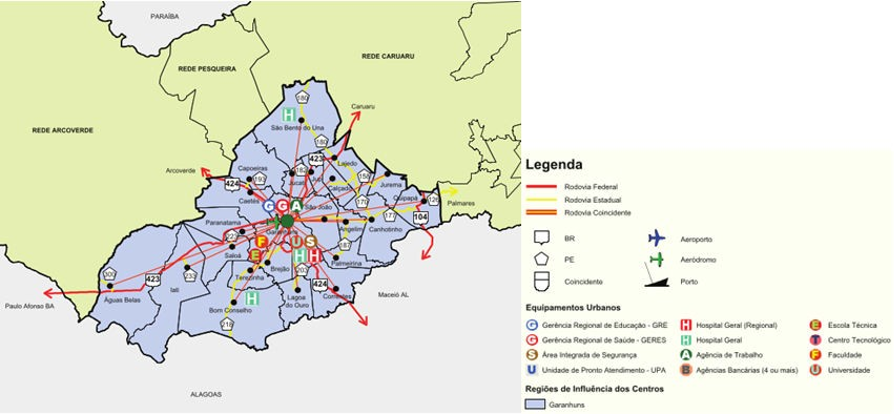
\includegraphics[width=\textwidth]{images/centralidade.png}
    \nota[Fonte]{Agência CONDEPE/FIDEM (2017)}
\end{figure}


A cidade de Garanhuns funciona como uma rede primaz, onde não há outros pólos de influência à sua proximidade. Essa rede urbana compreende 7,49\% do território estadual e influencia diretamente 12,43\ dos municípios pernambucanos. O que representa 3,57\% do PIB do Estado, onde o núcleo (Garanhuns) representa 33,57\% do PIB da rede (CONDEPE/FIDEM, 2017).

A ideia de criar um curso na área de computação existiu desde a concepção da Unidade Acadêmica de Garanhuns em setembro de 2005, quando começaram a funcionar 4 (quatro) cursos de graduação: Agronomia, Licenciatura Normal Superior (transformada no curso de Licenciatura em Pedagogia), Medicina Veterinária e Zootecnia. Em reunião geral, ocorrida em dezembro de 2007, ficou decidido em processo de votação que seria proposta a criação de 3 (três) novos cursos dentro do processo de Reestruturação Universitária (REUNI). Entre eles foi indicado o curso de Bacharelado em Ciência da Computação (BCC), no turno noturno, com o objetivo tanto de suprir a necessidade de um curso na área de computação, quanto proporcionar o desenvolvimento acadêmico da Universidade mediante uma forte interação com os demais cursos de graduação da UAG.

Além de interagir com as demais áreas da UAG, o curso de Bacharelado em Ciência da Computação veio atender a uma demanda regional identificada junto ao poder público local e à população. Portanto, o curso foi inserido dentro do contexto dos demais cursos da área de computação da UFRPE, de forma a contribuir com o desenvolvimento da UAG e dentro da realidade local. Para tanto, foram definidas áreas de atuação dos profissionais do curso bem como áreas de conhecimento que pudessem ser utilizadas para as outras áreas de conhecimentos já existentes na realidade da UAG-UFRPE.

De forma paralela, ressaltando a importância da  expansão  tecnológica,  constata-se que o uso do computador deixou de ser um diferencial para se tornar necessidade fundamental, tanto no contexto profissional quanto no dia a dia das pessoas. O advento da Internet transformou as tecnologias em elemento chave na construção da chamada sociedade da informação, modificando inclusive a forma de relacionamento na sociedade moderna. Dados de 2016 demonstram que existem no mundo cerca de 3.9 bilhões de usuários da Internet (ITU, 2018), e no Brasil a rede atende a aproximadamente 122 milhões de usuários.

O Brasil sofre com graves problemas tanto no acesso da população aos recursos computacionais quanto nas desigualdades regionais. Junto com a Internet surgem novas oportunidades de desenvolvimento ligadas à produção de conteúdo para a rede, aliados ao desenvolvimento de sistemas que usam grande quantidade de dados. Neste aspecto, é urgente a formação de profissionais ligados ao desenvolvimento de software. Nesse contexto, em 2006, a Sociedade Brasileira de Computação (SBC) definiu cinco grandes desafios atuais da computação:

\begin{enumerate}
    \item Gestão da informação em grandes volumes de dados multimídia distribuídos;
    \item Modelagem computacional de sistemas complexos artificiais, naturais, socioculturais e da interação homem-natureza;
    \item Impactos na computação da transição do silício para novas tecnologias;
    \item Acesso participativo universal do cidadão brasileiro ao conhecimento; e
    \item Sistemas disponíveis, corretos, seguros, escalonáveis, persistentes e ubíquos.
\end{enumerate}
	
Dentro desses desafios, pode-se contextualizar o curso de BCC da UAG em uma região carente de profissionais na área de desenvolvimento de software. Além disso, há o fato de haver, nessa região, claras possibilidades de aproveitamento dos profissionais a serem formados no ensino superior ofertado em Garanhuns. Com isso, obtêm-se a participação sócio-econômica dos atuais egressos das diferentes áreas técnicas científicas e informacionais (bacharéis, licenciados) em diversos municípios da região.

Adicionalmente, a região onde se encontra a UAG tem uma economia com base na agropecuária, e o município de Garanhuns tem uma forte atuação no setor de serviços, com forte apelo para o uso da Computação. Assim, a Computação é também um dos eixos norteadores do desenvolvimento municipal pelo fato do programa de expansão das universidades federais centrar-se na possibilidade de responder às demandas regionais sem, no entanto, restringir-se apenas à região, mas produzindo e transferindo conhecimentos, que é função inerente a toda Universidade.

Portanto, o curso de Bacharelado em Ciência da Computação foi projetado com eixos fundamentados em áreas do conhecimento que viessem a contribuir no desenvolvimento regional.

\section{Resultados Obtidos}

Em dezembro de 2015, o curso de Bacharelado em Ciência da Computação da UAG/UFRPE obteve a nota máxima de avaliação do ENADE (Exame Nacional de Desempenho dos Estudantes), ou seja, conceito 5. Isso fortalece a qualidade do desempenho dos estudantes com relação aos conteúdos programáticos previstos na diretriz curricular do curso, bem como o desenvolvimento de competências e habilidades necessárias ao aprofundamento da formação geral e profissional, e o nível de atualização dos estudantes com relação à realidade brasileira e mundial.

O curso de BCC foi avaliado com 4 estrelas (máximo de 5), sendo considerado Muito Bom nas duas últimas edições da Avaliação de Cursos Superiores do Guia do Estudante (GE), da Editora Abril em 2017 e 2018. Essa avaliação consta na publicação GE Profissões Vestibular 2018 e 2019.

O curso hoje é formado por 30 professores com dedicação exclusiva, distribuídos por formação e atuação nas principais áreas de conhecimento da Ciência da Computação, sendo aproximadamente 25 doutores e 5 mestres (doutorandos). Além disso, também contamos com professores das áreas de Matemática e Física. Atualmente o curso concorre e costumeiramente é contemplado com bolsas para projetos de pesquisa, extensão e iniciação tecnológica, como também possui grupos de pesquisa que tem gerado diversos artigos publicados por meio de trabalhos realizados com os discentes. Além de artigos, o curso promove melhorias na região por meio dos projetos de extensão que atende a diversas áreas, como projetos interdisciplinares em parceria com os outros cursos. Podemos citar alguns projetos, como: o desenvolvimento de aplicativos móveis para auxiliar agricultores e agrônomos nos processos de mecanização agrícola e para o ensino de química básica e avançada; soluções inteligentes para automatizar a irrigação de pequenos produtores rurais da região; ensino de programação básica para alunos de nível médio; e ensino de informática básica para a terceira idade.

O Centro de Tecnologia da Informação do Agreste Meridional de Pernambuco (Time JR.) é a Empresa Júnior do curso de Bacharelado em Ciência da Computação da UAG/UFRPE. A Time JR. é uma empresa formal composta por discentes de BCC, sob a orientação dos docentes, atuando como desenvolvedora de soluções para as diversas áreas do conhecimento e demanda da sociedade, atuando desde 2012 na região. 

Tomando por base o potencial criador e criativo que a conjuntura local oferece, como curso de Ciência da Computação, demais cursos e sociedade como um todo, e claro, da imensa demanda institucional e local represada, dois projetos foram criados para atuarem nesse cenário, o primeiro se refere a um Laboratório de Pesquisa e Desenvolvimento, chamado de BCC Coworking\footnote{\url{http://bcc.uag.ufrpe.br/bcccoworking}}, que é uma iniciativa exclusiva do curso de Computação, que surgiu com o propósito de servir como um local propício para o desenvolvimento de projetos reais, servindo até como fomento, com supervisão de profissionais da área, garantindo o conhecimento e a experiência técnica, através do uso de práticas e ferramentas do mercado de trabalho. É um ambiente onde o discente tem a oportunidade trazer sua ideia/projeto, de criar, manter e aumentar o \textit{networking} com outras pessoas de diversas áreas. É um local para aperfeiçoamento da produtividade. É importante destacar que não se trata de um espaço físico apenas, é principalmente um ambiente destinado aos estudantes em busca de conhecimento, experiência técnica, autonomia, fomentação e desenvolvimento de projetos. 

O segundo, diz respeito ao Laboratório Multidisciplinar de Tecnologias Sociais\footnote{\url{http://lmts.uag.ufrpe.br/}} (LMTS), como um espaço permanente de ensino, pesquisa, inovação tecnológica, extensão e de colaboração com a gestão institucional, contando com colaboradores da área técnica, mas também das demais áreas citadas, sejam eles, professores, técnicos ou estudantes. Este espaço agrega esta inteligência coletiva e as múltiplas iniciativas em curso ou idealizadas em prol especificamente para o desenvolvimento de \textit{softwares} livres ou públicos para atender as demandas da UFRPE e da sociedade em geral. O referido laboratório funciona com um propósito sem fins lucrativos, diferentemente da Time JR. (supracitada) e do BCC Coworking.

Atualmente, no contexto do curso de Ciência da Computação desta instituição, existem 7 (sete) grupos de pesquisa, liderados e coordenados por professores do curso. Estes grupos atuam nas grandes áreas da computação (Engenharia de Software, Inteligência Artificial, Banco de Dados, Redes de Computadores e Sistemas Distribuídos, Informática e Educação, entre outras) e desenvolvem atividades de pesquisa, monitoria, ensino e extensão.

\section{Categorias de cursos da área de computação e informática}

Com as diretrizes curriculares de 1999, foi criada a denominação da área de computação e informática orientando a elaboração do projeto político pedagógico dentro do tipo de curso escolhido. Assim, foram limitadas as possibilidades de nomes de cursos dessa área a 05 (cinco) tipos: Bacharelado em Ciência da Computação, Engenharia da Computação, Bacharelado em Sistemas da Informação, Cursos de Licenciatura em Computação e Cursos Superiores Tecnológicos, e posteriormente, o de Engenharia de Software. Segundo as diretrizes, esses cursos se enquadram em 04 (quatro) categorias básicas:

\begin{enumerate}
    \item Cursos que têm a computação como atividade-fim: Ciência da Computação e Engenharia da Computação;
    \item Cursos que têm a informática como atividade-meio:  Sistema da Informação;
    \item Cursos voltados para o ensino da informática: Licenciatura em Computação; e,
    \item Cursos Tecnológicos e sequenciais.
\end{enumerate}

Para que o curso escolhido se inserisse melhor dentro do desenvolvimento da UAG, optou-se pelo curso de Bacharelado em Ciência da Computação (BCC) que se enquadra na categoria de curso com a computação como atividade-fim.

O curso de BCC da UAG foi idealizado a partir do currículo de referência formulado em documento de 2005 pela IEEE Computer Society (Instituto de Engenheiros Eletricistas e Eletrônicos), e levando em conta as tendências e desafios para a área de informática descrita em publicação sobre a trajetória dos cursos de graduação da área de computação e informática publicada pela Sociedade Brasileira de Computação (SBC). A matriz curricular foi construída a partir do estudo de projetos de cursos de outras Instituições de Ensino Superior, de alto nível, seguindo as recomendações do Currículo de Referência da Sociedade Brasileira de Computação (1999) e as diretrizes de 2012 e 2016 do MEC.

Este Projeto Pedagógico vem sendo construído e revisado desde o final de 2015, com encontros mensais por parte do NDE, sendo inicialmente os encontros com todo o quadro docente do curso, com intuito de um planejamento mais robusto, que se tornasse duradouro. A partir de 2016 com reuniões mensais, uma proposta mais robusta foi sendo consolidada. Essa proposta no decorrer dos anos vem sendo continuamente ajustada e atualizada pelos membros do NDE. Entre as várias dificuldades encontradas pelo NDE para dar prosseguimento ao projeto, as principais foram, realizar um estudo mais profundo para entender e embasar a decisão do curso de se tornar vespertino, como também, mudanças nas resoluções da Sociedade Brasileira da Computação e do Ministério da Educação. E, do ano de 2018 em diante, sofrendo as adequações exigidas pelas Pró-reitoria de Ensino e Graduação, tendo essa pró-reitoria também enfrentado mudanças nesse período na abordagem de construção dos PPCs.


\chapter{OBJETIVOS DO CURSO}

A Ciência da Computação é uma área de atuação bem diversa, uma vez que o profissional pode atuar em diferentes segmentos, inclusive, apenas na aplicação da computação como meio para outras áreas do conhecimento. O curso de BCC tem como objetivo formar profissionais com bases científicas e tecnológicas na área da computação, capazes de resolver problemas dos mais diferentes domínios, através de métodos e técnicas computacionais, para atuar de forma bem sucedida tanto na área acadêmica quanto no mercado de trabalho. 

Os objetivos específicos do curso são:

\begin{enumerate}
    \item Desenvolver nos estudantes o perfil científico de pesquisador, tanto para atuação na área acadêmica, quanto para atuação em outros ramos de atividade;
    \item Desenvolver nos estudantes um espírito empreendedor, incentivando e motivando a sua independência e criatividade;
    \item Desenvolver nos discentes o perfil para trabalhar na indústria, aplicando os seus conhecimentos técnicos de desenvolvimento de software e soluções para TI;
    \item Promover a interdisciplinaridade buscando atualização constante na área de computação;
    \item Motivar e orientar o estudante para que ele tenha uma postura ativa diante da necessidade de um aprendizado contínuo e autônomo;
    \item Promover uma postura ética e socialmente comprometida com o papel do estudante no desenvolvimento científico, tecnológico, social e econômico da sua região e do País;
    \item Promover interação constante com escolas do ensino fundamental e médio local, de forma a estimular vocações e colaborar ativamente com a melhoria da educação.
    
\end{enumerate}

\chapter{PERFIL PROFISSIONAL DO EGRESSO}

Deve se interessar pela computação e, em particular, pela ciência. Deve possuir entusiasmo para conhecer e dominar novos assuntos, além de disposição para construir sua própria reputação por meio dos produtos do esforço próprio ou resultantes de trabalho em equipe do qual participa. Deve possuir atitude e a necessidade de realizar, mesmo sem supervisão. Deve engajar-se em representações locais, regionais, nacionais e internacionais, através de representações de classe, visando a atualização e fortalecimento da sociedade. Estes atributos são esperados na conduta do estudante ingressante e utilizados ao longo do curso.

\section{Descrição dos requisitos psicofísicos}

Para atender ao perfil profissional definido, as atividades do curso priorizam o exercício dos requisitos inerentes ao desempenho da profissão, a citar:

\begin{itemize}
    \item Método e disciplina de trabalho;
    \item Raciocínio lógico e abstrato;
    \item Capacidade de trabalho em equipe;
    \item Criatividade, produtividade e iniciativa;
    \item Disposição para efetuar trabalho complexo e minucioso;
    \item Compromisso com o desenvolvimento tecnológico;
    \item Compromisso com o ser humano;
    \item Senso crítico, seriedade e responsabilidade.
\end{itemize}

\section{Egresso}

Do egresso de um curso de Bacharelado em Ciência da Computação é exigida uma predisposição e aptidões para a área, além de um conjunto de competências, habilidades e atitudes a serem adquiridas durante a realização do curso. Como perfil do Egresso, espera-se que ele ao final do curso, o profissional de Ciência da Computação necessita de flexibilidade para atender domínios diversificados de aplicação e as vocações institucionais. Dessa maneira, espera-se que os egressos desses cursos:

\begin{enumerate}
    \item Possuam sólida formação em Ciência da Computação e Matemática, que os capacitem a construir aplicativos de propósito geral, ferramentas e infraestrutura de software de sistemas de computação e de sistemas embarcados, gerar conhecimento científico e inovação, e que os incentivem a estender suas competências à medida que a área se desenvolve;
    \item Adquiram visão global e interdisciplinar de sistemas e entendam que esta visão transcende os detalhes de implementação dos vários componentes e os conhecimentos dos domínios de aplicação;
    \item Conheçam a estrutura dos sistemas de computação e os processos envolvidos na sua construção e análise;
    \item Dominem os fundamentos teóricos da área de Computação e como eles influenciam a prática profissional;
    \item Sejam capazes de agir de forma reflexiva na construção de sistemas de computação, compreendendo o seu impacto direto ou indireto sobre as pessoas e a sociedade;
    \item Sejam capazes de criar soluções, individualmente ou em equipe, para problemas complexos caracterizados por relações entre domínios de conhecimento e de aplicação.
\end{enumerate}

\section{Definição do perfil profissional}

Por definição, o Bacharel em Ciência da Computação deve ser um profissional qualificado para a pesquisa e desenvolvimento na área de computação, para o projeto e construção de hardware e software básico e também para o uso de sistemas computadorizados em outras áreas da atividade humana, a fim de viabilizar ou aumentar a produtividade e a qualidade de todos os tipos de procedimentos. Na UFRPE todo egresso deve ser um profissional: (1) com domínio e capacidade para trabalhar na área da Computação, desenvolvendo projetos de computadores e sistemas de computação, programas e sistemas de informação; (2) atento ao caráter ecológico, social e ético; e (3) que exerça suas atividades na sociedade com responsabilidade.

Adaptadas de documentos propostos pela ACM/IEEE e SBC, seguem as competências e habilidades necessárias para o egresso profissional de Ciência da Computação:

\begin{itemize}
    \item Possuir capacidade de raciocínio lógico e abstrato;
    \item Capacidade de utilizar conhecimentos de matemática, física, ciência da computação, engenharia e tecnologias modernas no apoio à construção de produtos e serviços seguros, confiáveis e de relevância social;
    \item Identificar práticas apropriadas dentro de um quadro ético, legal e profissional;
    \item Capacidade de atuar profissionalmente com ética avaliando o impacto de suas atividades no contexto social e ambiental;
    \item Reconhecer a necessidade de um desenvolvimento profissional contínuo;
    \item Capacidade para aprender a aprender. O aluno precisará estar sempre aprendendo para se manter atualizado e competente. A habilidade em pesquisa está fortemente relacionada com o auto-aprendizado;
    \item Discutir e explicar aplicações baseadas no corpo de conhecimento da computação;
    \item Visão sistêmica da área de computação;
    \item Profundo conhecimento dos aspectos teóricos, científicos e tecnológicos relacionados à área de computação;
    \item Demonstrar habilidade para trabalhar como um indivíduo sob orientação, como um membro de uma equipe ou como líder de uma equipe;
    \item Eficiência na operação de equipamentos computacionais e sistemas de software;
    \item Competência para identificar, analisar e documentar oportunidades, problemas e necessidades passíveis de solução via computação, e para empreender na concretização desta solução;
    \item Capacidade para pesquisar e viabilizar soluções de software para várias áreas de conhecimento e aplicação, como, por exemplo, desenvolvimento e/ou aprimoramento de protocolos de comunicação, modelos matemáticos-computacionais, técnicas de armazenamento de dados, construção de linguagens de programação, dentre inúmeras outras;
    \item Capacidade de abstração quando desenvolvendo as atividades de programação, projeto e modelagem;
    \item Compreender e aplicar conceitos, princípios e práticas essenciais no contexto de cenários bem definidos, mostrando discernimento na seleção e aplicação de técnicas e ferramentas;
    \item Compreensão da importância de se valorizar o  usuário  no  processo  de  interação com sistemas computacionais e competência na utilização de técnicas de interação homem-máquina neste processo;
    \item Conhecimento de aspectos relacionados à evolução da área de computação, de forma a poder compreender a situação presente e projetar a evolução futura;
    \item Capacidade para desenvolvimento de pesquisa científica e tecnológica, que permita ao aluno ingressar em um curso de pós-graduação ou realizar estas pesquisas na indústria;
    \item Capacidade de avaliar de forma aprofundada e com embasamento teórico as atividades realizadas e produtos desenvolvidos. Esta habilidade pode ser desenvolvida através de atividades de leitura e discussão de temas e elaboração de painéis de discussão com profissionais da área;
    \item Capacidade para conceber soluções inovadoras para tornar produtos competitivos;
    \item Capacidade de, com base nos conceitos adquiridos, iniciar, projetar, desenvolver, implementar, validar e gerenciar qualquer projeto de software. Este trabalho exige habilidade de solução de problemas e de avaliação crítica;
    \item Capacidade para projetar e desenvolver sistemas que integram hardware e software;
    \item Capacidade para avaliar prazos e custos em projetos de software;
    \item Competência e compromisso com a utilização de princípios e ferramentas que reduzam o tempo de desenvolvimento e implementação de um projeto e lhe confiram um alto grau de qualidade;
    \item Aplicação eficiente dos princípios de gerenciamento, organização e busca de informações;
    \item Conhecimento de aspectos relacionados às tecnologias de mídias digitais;
    \item Habilidade de lidar com notações, linguagens e ferramentas para elaboração de modelos;
    \item Capacidade empreendedora, inclusive para aqueles que não desejam ser empresários. Esta habilidade capacita o profissional a tomar iniciativas e a liderar projetos em suas atividades profissionais. Ela é desenvolvida nos alunos através de projetos nos quais eles são estimulados a apresentar e liderar projetos de sistemas;
    \item Capacidade de se expressar bem de forma oral ou escrita usando a língua portuguesa através da elaboração e apresentação de projetos e monografias durante todo o curso;
    \item Fluência na língua inglesa suficiente para a leitura e compreensão de documentos técnicos na área de computação.
    \item O aluno deve desenvolver competência e desempenho em língua inglesa através de disciplinas complementares e leitura de livros e artigos de computação escritos em Inglês, que são exigidos em várias atividades curriculares. 
\end{itemize}

\chapter{CAMPO DE ATUAÇÃO PROFISSIONAL}

Na contemporaneidade tem-se exigido respostas céleres a problemas complexos decorrentes do mundo globalizado, no qual a informação adquire um papel proeminente. Não é por acaso que o atual modo de vida das pessoas está intrinsecamente ligado ao uso das tecnologias, em especial, dos computadores. Estes podem ser encontrados nos mais variados lugares, como, por exemplo, nos lares (em TV's, eletrodomésticos, vídeo games), escolas (PC's, tablets, laboratórios), indústria (equipamentos de segurança, relógios-ponto, máquinas), comércio (caixas registradoras), dentre outros. 

Desta forma, o profissional atuará possivelmente nos seguintes problemas:

\begin{itemize}
    \item concepção, especificação, projeto, construção, avaliação e adaptação de sistemas digitais;
    \item análise e projeto de estrutura lógica e funcional de computadores e sua implementação;
    \item desenvolvimento e implementação de software básico e de apoio para sistemas computacionais;
    \item projeto e desenvolvimento de sistemas e programas usando linguagens de programação;
    \item projeto e desenvolvimento de sistemas de estruturação de informação;
    \item projeto e desenvolvimento de redes de processamento local e remota, em matéria de hardware e de software.    
\end{itemize}

O egresso do curso de Bacharelado em Ciência da Computação deve estar preparado para propor soluções inovadoras e adequadas para problemas propostos, capacitado a acompanhar e avaliar avanços tecnológicos em computação, bem como aplicar e implementar as evoluções, reposições e adaptações que se façam necessárias, tanto de forma reativa como pró-ativa, logo deve estar apto a desenvolver as seguintes funções no mercado de trabalho:

\begin{itemize}
    \item \textbf{Empreendedor} – descobrimento e empreendimento de novas oportunidades para aplicações usando sistemas computacionais e avaliando a conveniência de se investir no desenvolvimento da aplicação;
    \item \textbf{Consultor} – consultoria e assessoria a empresas de diversas áreas no que tange ao uso adequado de sistemas computacionais;
    \item \textbf{Coordenador de equipe} – coordenação de equipes envolvidas em projetos na área de computação e informática;
    \item \textbf{Membro de equipe} – participação de forma colaborativa e integrada de equipes que desenvolvem projetos na área de informática;
    \item \textbf{Pesquisador} – participação em projetos de pesquisa científica e tecnológica. 
\end{itemize}

\chapter{REQUISITOS DE INGRESSO}

O curso de Bacharelado em Ciência da Computação tem duas entradas anuais com 40 vagas por semestre letivo, resultando em 80 vagas por ano. O ingresso dos alunos ocorre através do Sistema de Seleção Unificado – SISU, com base nos resultados obtidos no Exame Nacional do Ensino Médio – ENEM, e do Ingresso Extra.

\begin{enumerate}
    \item \textbf{Ingresso através do ENEM}: a UFRPE adota o SISU como principal meio de acesso aos cursos de graduação, através da nota do ENEM, considerando as duas entradas semestrais.
    \item \textbf{Ingresso Extra}: além do ingresso semestral, a partir da seleção do SISU, a UFRPE possui outras modalidades de acesso. Estas ocorrem duas vezes por ano, em datas previstas e com editais publicados pela Pró-Reitoria de Ensino de Graduação – PREG. 
\end{enumerate}

Nessa direção, são modalidades de ingresso extra:

\begin{itemize}
    \item \textbf{Reintegração} – Após ter perdido o vínculo com a Universidade, o aluno que tenha se evadido pelo período máximo de integralização de seu curso poderá requerer a reintegração, uma única vez, no mesmo curso (inclusive para colação de grau), desde que tenha condições de concluí-lo no prazo máximo permitido (considerando o prazo do vínculo anterior e o que necessitará para a integralização do currículo) e que não possua 4 (quatro) ou mais reprovações em uma mesma disciplina (Fundamentação: Res. CEPE/UFRPE nº 100/83 (de 16 de setembro de 1983) e Resolução CEPE/UFRPE nº 354/2008 (de 13 de junho de 2008).
    \item \textbf{Reopção ou Transferência Interna} – O aluno regularmente matriculado que esteja insatisfeito com o seu curso poderá requerer a transferência interna para outro curso de graduação desta Universidade. Para tanto, ele deverá considerar: a área de conhecimento afim ao seu curso de origem; a existência de vagas no curso pretendido; o cumprimento de, no mínimo, 40\% (quarenta por cento) do currículo original do seu curso, dispondo, portanto, de tempo para integralização curricular, considerando os vínculos com o curso anterior e o pretendido (Fundamentação: Res. CEPE/UFRPE nº 34/97, de 16/01/1997).
    \item \textbf{Transferência Externa} – A Universidade recebe alunos de outras IES, vinculados a cursos reconhecidos pelo CNE, desde que eles: desejem continuar o curso iniciado ou ingressar em curso de área afim; estejam com vínculo ativo ou trancado com a Instituição de origem; tenham condições de integralizar o currículo no seu prazo máximo, considerando, também, o prazo definido pela outra IES e o que necessitaria cursar na UFRPE; e, por fim, que tenham cursado todas as disciplinas constantes do primeiro período da matriz curricular do curso pretendido na UFRPE. Salvo os casos de transferência ex-officio (que independem de vagas), é necessário, para ingresso, que o curso tenha vagas ociosas (Fundamentação: Res. CEPE/ UFRPE nºs 124/83 e 180/91).
    \item \textbf{Portadores de Diploma de Curso Superior} – Os portadores de diploma de curso superior, reconhecido pelo CNE, que desejem realizar matrícula em outro curso superior na UFRPE, em área afim, podem requerê-la, desde que haja disponibilidade após o preenchimento de vagas pelas demais modalidades de ingresso. (Fundamentação: Res. CEPE/UFRPE nº 181/91, de 01/10/1991).
\end{itemize}

As formas de ingresso definidas a seguir independem de vagas e não há necessidade de publicação de edital da PREG:

\begin{itemize}
    \item \textbf{Cortesia Diplomática} – Em atendimento ao que preconiza o Decreto nº 89.758/84, de 06/06/84, a UFRPE aceita alunos incluídos nas seguintes situações: funcionário estrangeiro, de missão diplomática ou repartição consular de carreira no Brasil, e seus dependentes legais; funcionário estrangeiro de Organismo Internacional que goze de privilégios e imunidades em virtude de acordo entre o Brasil e a organização, e seus dependentes legais; técnico estrangeiro, e seus dependentes legais, que preste serviço em território nacional, no âmbito de acordo de cooperação cultural, técnica, científica ou tecnológica, firmado entre o Brasil e seu país de origem, desde que em seu contrato esteja prevista a permanência mínima de 1 (um) ano no Brasil; e, finalmente, técnico estrangeiro, e seus dependentes legais, de organismo internacional, que goze de privilégios e imunidades em virtude de acordo entre o Brasil e a organização, desde que em seu contrato esteja prevista a permanência mínima de 1 (um) ano em território nacional.

    Este tipo de ingresso nos cursos de graduação se dá mediante solicitação do Ministério das Relações Exteriores, encaminhada pelo MEC, com a isenção de processo seletivo e independentemente da existência de vagas, sendo, todavia, somente concedido a estudantes de países que assegurem o regime de reciprocidade e que sejam portadores de visto diplomático ou oficial.

    \item \textbf{Programa de Estudantes-Convênio de Graduação (PEC-G)} – Alunos provenientes de países em desenvolvimento, especialmente da África e da América Latina, são aceitos como estudantes dos cursos de graduação da UFRPE. Estes estudantes são selecionados, por via diplomática em seus países, considerando os mecanismos previstos no protocolo do PEC-G e obedecendo aos princípios norteadores da filosofia desse Programa. Não pode ser admitido, através desta modalidade, o estrangeiro portador de visto de turista, diplomático ou permanente, bem como o brasileiro dependente dos pais que, por qualquer motivo, estejam prestando serviços no exterior, e o indivíduo com dupla nacionalidade, sendo uma delas brasileira.
    \item {\bfseries Transferência Obrigatória ou \textit {ex officio}} – É a Transferência definida na Lei n.º 9.536, de 11/12/97 que regulamenta o Art. 49 da Lei n.º 9.394, de 20/12/96, Portaria Ministerial nº 975/92, de 25/06/92 e Resolução nº 12, de 02/07/94 do Conselho Federal de Educação - CFE. Esta transferência independe da existência de vaga e época, abrangendo o servidor público federal da administração direta ou indireta, autárquica, fundacional ou membro das Forças Armadas, regidos pela Lei n.º 8.112/90, inclusive seus dependentes, quando requerido em razão de comprovada remoção ou transferência \textit {ex officio}. A transferência deverá implicar em mudança de residência para o município onde se situe a instituição recebedora ou para localidade próxima a esta, observadas as normas estabelecidas pelo CNE.
\end{itemize}

\chapter{ORGANIZAÇÃO CURRICULAR}

Levando em consideração as orientações contidas na Resolução CNE/CES num. 5 de 11/2016, que institui as Diretrizes Curriculares Nacionais para os cursos de graduação na área da Computação, o currículo do curso de Bacharelado em Ciência da Computação apresenta a seguinte estrutura conforme Quadro 3 abaixo:

\begin{center}
  \begin{scriptsize}
    \begin{longtable}{@{}lp{10cm}}
      \caption{\label{quadro:organizacao-curricular-do-curso}Organização curricular do curso.}\\
    \toprule
    \textbf{Núcleo de Conhecimento} & \textbf{Componentes Curriculares} \\ 
    \midrule
    Conteúdos Básicos & PRÉ-CÁLCULO\\ 
                      & LÓGICA MATEMÁTICA \\
                      & COMPUTADORES E SOCIEDADE \\
                      & INGLÊS  \\
                      & CÁLCULO I \\
                      & GEOMETRIA ANALÍTICA \\
                      & METODOLOGIA CIENTÍFICA \\
                      & INGLÊS INSTRUMENTAL \\
                      & CÁLCULO II \\
                      & ÁLGEBRA LINEAR I \\
                      & MATEMÁTICA DISCRETA PARA COMPUTAÇÃO \\
                      & PROBABILIDADE E ESTATÍSTICA \\
                      & FÍSICA PARA COMPUTAÇÃO \\ \midrule
    Conteúdos Tecnológicos  & INTRODUÇÃO À CIÊNCIA DA COMPUTAÇÃO \\ 
                            & INTRODUÇÃO À PROGRAMAÇÃO \\
                            & ALGORITMOS E ESTRUTURA DE DADOS II \\
                            & PROGRAMAÇÃO ORIENTADA A OBJETOS \\
                            & ALGORITMOS E ESTRUTURA DE DADOS \\
                            & SISTEMAS DIGITAIS \\
                            & PARADIGMAS DE LINGUAGENS DE PROGRAMAÇÃO \\
                            & INTERAÇÃO HUMANO COMPUTADOR \\
                            & BANCO DE DADOS \\
                            & INTELIGÊNCIA ARTIFICIAL \\
                            & ARQUITETURA DE COMPUTADORES \\
                            & PROJETO E ANÁLISE DE ALGORITMOS \\
                            & REDES DE COMPUTADORES \\
                            & SISTEMAS OPERACIONAIS \\
                            & TEORIA DA COMPUTAÇÃO \\
                            & COMPUTAÇÃO GRÁFICA \\
                            & ENGENHARIA DE SOFTWARE \\
                            & SISTEMAS DISTRIBUÍDOS \\
                            & EMPREENDIMENTOS EM TIC \\
                            & PROJETO DE DESENVOLVIMENTO DE SOFTWARE \\
                            & PROGRAMAÇÃO WEB \\
                            & SISTEMAS DE INFORMAÇÃO E TECNOLOGIAS \\
                            & APRENDIZAGEM DE MÁQUINA \\
                            & PROCESSAMENTO DIGITAL DE IMAGENS \\
                            & COMPILADORES \\
                            & ESTÁGIO SUPERVISIONADO OBRIGATÓRIO \\
                            & TRABALHO DE CONCLUSÃO DE CURSO I \\
                            & TRABALHO DE CONCLUSÃO DE CURSO II \\
    \bottomrule
    \end{longtable}
  \end{scriptsize}      
\end{center}

A carga horária total do curso de Bacharelado em Ciência da Computação tem um total de 3.200h horas, sendo distribuída em 4,5 (quatro vírgula cinco) anos, isto é, 9 (nove) períodos. Os conteúdos de formação serão apresentados em componentes curriculares com carga horária variando entre 30h e 60h para as disciplinas, 300h para ESO e para TCC 1 60h e TCC 2 180h. Cada hora-aula corresponde a 60 minutos, conforme expresso na Resolução CEPE/UFRPE nº 220/2016 e demonstrado no Quadro 4 abaixo.

\begin{center}
  
  \begin{scriptsize}
    \begin{longtable}{p{4cm}p{1.5cm}p{2cm}p{3cm}}
      \caption{\label{quadro:distribuicao-nucleos-formacao-e-ch}Distribuição dos núcleos de formação e carga horária.}\\
    \toprule
    \multicolumn{4}{c}{\textbf{Bacharelado em Ciência da Computação}}\\ \midrule
    \multicolumn{2}{l}{\textbf{Núcleo}} & \multicolumn{1}{c}{\textbf{Carga Horária (h)}} & \multicolumn{1}{c}{\textbf{\%}}\\
    \midrule
    Básicos & & \multicolumn{1}{c}{660} & \multicolumn{1}{r}{20,6}\\ \midrule
    \multirow{3}{3cm}{Tecnológico / Profissionalizante} & Disciplinas & \multicolumn{1}{c}{1.440} & \multicolumn{1}{r}{45,0}\\ \cline{2-4}
    & TCC & \multicolumn{1}{c}{180} & \multicolumn{1}{r}{5,6}\\ \cline{2-4}
    & ESO & \multicolumn{1}{c}{300} & \multicolumn{1}{r}{9,4}\\ \midrule
    \multicolumn{2}{l}{Componentes optativos} & \multicolumn{1}{c}{300} & \multicolumn{1}{r}{9,4}\\ \midrule
    \multicolumn{2}{l}{Atividades complementares} & \multicolumn{1}{c}{320} & \multicolumn{1}{r}{10,0}\\ \midrule
    \multicolumn{2}{l}{Total} & \multicolumn{1}{c}{3.200} & \multicolumn{1}{r}{100,0}\\
\bottomrule
\end{longtable}
\end{scriptsize}      
\end{center}

Para obtenção do título em Bacharel em Ciência da Computação o aluno deverá cumprir uma carga horária total de 3.200h horas, entre disciplinas, atividades complementares, Trabalho de Conclusão de Curso e Estágio Obrigatório Supervisionado. O discente terá a possibilidade de cursar disciplinas do ciclo básico e disciplinas do ciclo tecnológico/profissional, podendo ainda escolher em qual área deseja se aprofundar, uma vez que pode escolher entre as disciplinas optativas que necessita cursar.

As disciplinas de um mesmo período letivo ou de períodos anteriores, no qual o aluno tenha cursado, devem se articular em torno de um ou mais projetos de natureza interdisciplinar, buscando otimizar o processo de avaliação nas disciplinas e uma melhor adequação do esforço para resolução de problemas por parte dos discentes, uma vez que assim eles concentram seus esforços num único projeto que contempla aquelas disciplinas que naturalmente interagem. As disciplinas, em suas atividades e projetos, são baseadas na metodologia de aprendizagem baseada em projetos (\textit{Project Based Learning} (PBL) [Barrows, 1986]). Além do diálogo entre as disciplinas, o curso estará atento à tentativa de promoção de uma educação inclusiva, adaptando os conteúdos programáticos previstos em cada componente curricular em função das necessidades de aprendizagem dos estudantes.

Algumas disciplinas serão ofertadas de forma semipresencial, atendendo as exigências do MEC do artigo 7º, da portaria nº 1428/2018, cujos métodos e práticas de ensino-aprendizagem incorporarão Tecnologias de Informação e Comunicação - TICs para a realização dos objetivos pedagógicos (ver seção no 14, destinada à metodologia e avaliação).

Com relação a carga horária permitida para as disciplinas na modalidade semipresencial, atualmente o curso atende o percentual máximo de 20\% (vinte por cento) da carga horária total do curso ou das disciplinas no formato EAD, consoante a Portaria MEC nº 1.134/2016 e Resolução CEPE/UFRPE nº 220/2016. Porém, algumas disciplinas poderão ser ofertadas com até o percentual de 20\% na modalidade a distância, conforme a portaria nº 4.059/04 do MEC, desde que sejam apresentados os programas de disciplinas, métodos, formas de avaliação e acompanhamento e a justificativa.

O desenvolvimento de atividades práticas e visitas técnicas a organizações públicas, privadas e não governamentais, permitirá aos estudantes o contato com demandas e situações próprias da profissão. Esta, também incluirá, como etapa integrante da graduação, o ESO, sob a orientação direta da instituição de ensino, conforme disposto na seção 10. A carga horária do ESO será de 300 (trezentas) horas. Serão obrigatórias, ainda, as disciplinas de TCC, a primeira de 60 (sessenta) horas e a segunda de 120 (cento e vinte) horas. A participação no Exame Nacional de Desempenho de Estudantes (ENADE) é requisito indispensável para a integralização do curso, bem como a integralização de 300 horas de disciplinas optativas.

\section{Matriz curricular}

A matriz curricular busca atender os objetivos traçados e o perfil desejado do egresso em Ciência da Computação. Os componentes curriculares que serão ofertados no bacharelado estão distribuídos considerando a seguinte tipologia: obrigatórios (que corresponde àquelas que o aluno deve obrigatoriamente cursar ao longo dos semestres) e optativos (dentre o rol de disciplinas ofertadas, o aluno escolhe cursar aquelas de seu interesse). No Quadro 5 são expostos os períodos nos quais estes componentes estão dispostos no curso.

\begin{center}
  
  \begin{tiny}
    \begin{longtable}{cp{4.5cm}cccp{2.8cm}p{2.8cm}}
      \caption{\label{quadro:matriz-curricular-do-curso}Matriz Curricular do Curso de Bacharelado em Ciência da Computação.}\\
    \toprule
    \textbf{Per.} & \textbf{Disciplina} & \multicolumn{3}{c}{\textbf{Carga Horária}} & \textbf{Pré-requisitos} & \textbf{Correquisitos}\\
    & & \textbf{Teó.} & \textbf{Prát.} & \textbf{Total} & & \\
    \midrule
    1 & UAG00076 PRÉ-CÁLCULO & 60 & 0 & 60 & & \\ \cline{2-7}
      & MATM3008 LÓGICA MATEMÁTICA & 60 & 0 & 60  & &\\ \cline{2-7}
      & CCMP3057 INTRODUÇÃO À PROGRAMAÇÃO & 45 & 45 & 90  & &\\ \cline{2-7}
      & CCMP3056 INTRODUÇÃO À CIÊNCIA DA COMPUTAÇÃO & 30 & 0 & 30  & &\\ \cline{2-7}
      & CCMP3071 COMPUTADORES E SOCIEDADE & 15 & 15 & 30  & &\\ \cline{2-7}
      & LETR3020 INGLÊS & 30 & 0 & 30  & &\\ \midrule
      & \multicolumn{3}{l}{\textbf{Subtotal}} & \textbf{300} & & \\ \midrule
    2 & MATM3030 CÁLCULO I & 60 & 0 & 60 & PRÉ-CÁLCULO & \\ \cline{2-7}   
      & MATM3021 GEOMETRIA ANALÍTICA & 60 & 0 & 60 & & \\ \cline{2-7}
      & CCMP3070 INTERAÇÃO HUMANO COMPUTADOR & 30 & 30 & 60 & & \\ \cline{2-7}
      & CIEN3005 METODOLOGIA CIENTÍFICA & 30 & 0 & 30 & & \\ \cline{2-7}
      & INGLÊS INSTRUMENTAL & 30 & 0 & 30 &  \\ \cline{2-7}
      & CCMP3006 ALGORITMOS E ESTRUTURA DE DADOS I & 30 & 30 & 60 & INT. À PROGRAMAÇÃO & \\ \midrule
      & \multicolumn{3}{l}{\textbf{Subtotal}} & \textbf{300} & & \\ \midrule
    3 & MATM3006 CÁLCULO II & 60 & 0 & 60 & CÁLCULO I & \\ \cline{2-7}
      & ÁLGEBRA LINEAR I & 60 & 0 & 60 & GEOMETRIA ANALÍTICA & \\ \cline{2-7}
      & CCMP3016 ALGORITMOS E ESTRUTURA DE DADOS II & 30 & 30 & 60 & ALG. E EST. DE DADOS I & \\ \cline{2-7}
      & MATEMÁTICA DISCRETA PARA COMPUTAÇÃO & 60 & 0 & 60 & LÓGICA MATEMÁTICA & \\ \cline{2-7}
      & CCMP3017 PROGRAMAÇÃO ORIENTADA A OBJETOS & 30 & 30 & 60 & INT. À PROGRAMAÇÃO & \\ \midrule
      & \multicolumn{3}{l}{\textbf{Subtotal}} & \textbf{300} & & \\ \midrule
    4 & PRBE3006 PROBABILIDADE E ESTATÍSTICA & 60 & 0 & 60 & CÁLCULO II & \\ \cline{2-7}
      & FISC3004 FÍSICA PARA COMPUTAÇÃO & 60 & 0 & 60 & & \\ \cline{2-7}
      & CCMP3058 SISTEMAS DIGITAIS & 45 & 15 & 60 & & FÍSICA PARA COMPUTAÇÃO \\ \cline{2-7}
      & CCMP3065 PARADIGMAS DE LINGUAGENS DE PROGRAMAÇÃO & 45 & 15 & 60 & PROGRAMAÇÃO ORIENTADA A OBJETOS; \newline ALGORITMOS E ESTRUTURA DE DADOS I & \\ \cline{2-7}
      & CCMP3064 PROJETO E ANÁLISE DE ALGORITMOS & 30 & 30 & 60 & ALGORITMOS E ESTRUTURA DE DADOS 2 & \\ \midrule
      & \multicolumn{3}{l}{\textbf{Subtotal}} & \textbf{300} & & \\ \midrule
    5 & CCMP3010 ARQUITETURA DE COMPUTADORES & 45 & 15 & 60 & SISTEMAS DIGITAIS & \\ \cline{2-7}
      & CCMP3018 ENGENHARIA DE SOFTWARE & 30 & 30 & 60 & PROGRAMAÇÃO ORIENTADA A OBJETOS & \\ \cline{2-7}
      & CCMP3023 REDES DE COMPUTADORES & 30 & 30 & 60 & PROGRAMAÇÃO ORIENTADA A OBJETOS & \\ \cline{2-7}
      & CCMP3066 BANCO DE DADOS & 30 & 30 & 60 & MATEMÁTICA DISCRETA & \\ \cline{2-7}
      & ADMT3018 EMPREENDIMENTOS EM TIC & 60 & 0 & 60 & & \\ \cline{2-7}
      & APRENDIZAGEM DE MÁQUINA & 15 & 15 & 30 & PROBABILIDADE E ESTATÍSTICA e ALGORITMOS E ESTRUTURA DE DADOS II & \\ \midrule
      & \multicolumn{3}{l}{\textbf{Subtotal}} & \textbf{330} & & \\ \midrule
    6 & CCMP3067 SISTEMAS DE INFORMAÇÃO E TECNOLOGIAS & 60 & 0 & 60 & & \\ \cline{2-7}
      & CCMP3021 SISTEMAS DISTRIBUÍDOS & 30 & 30 & 60 & REDES DE COMPUTADORES & SISTEMAS OPERACIONAIS \\ \cline{2-7}
      & CCMP3009 SISTEMAS OPERACIONAIS & 45 & 15 & 60 & & \\ \cline{2-7}
      & CCMP3068 TEORIA DA COMPUTAÇÃO & 60 & 0 & 60 & MATEMÁTICA DISCRETA & \\ \cline{2-7}
      & PROCESSAMENTO DIGITAL DE IMAGENS & 15 & 15 & 30 & ALGORITMOS E ESTRUTURA DE DADOS II & APRENDIZAGEM DE MÁQUINA \\ \cline{2-7}
      & OPTATIVA I & & & 60 & & \\ \midrule
      & \multicolumn{3}{l}{\textbf{Subtotal}} & \textbf{330} & & \\ \midrule
    7 & CCMP3020 COMPILADORES & 45 & 15 & 60 & TEORIA DA COMPUTAÇÃO; \newline ALGORITMOS E ESTRUTURAS DE DADOS II & \\ \cline{2-7}
      & CCMP3014 INTELIGÊNCIA ARTIFICIAL & 30 & 30 & 60 & ALGORITMOS E ESTRUTURAS DE DADOS II & \\ \cline{2-7}
      & PROGRAMAÇÃO WEB & 30 & 30 & 60 & PROGRAMAÇÃO ORIENTADA A OBJETOS; \newline BANCO DE DADOS & \\ \cline{2-7}
      & OPTATIVA II & & & 60 & & \\ \cline{2-7}
      & OPTATIVA III & & & 60 & & \\ \midrule
      & \multicolumn{3}{l}{\textbf{Subtotal}} & \textbf{300} & & \\ \midrule
    8 & TRABALHO DE CONCLUSÃO DE CURSO I - CIÊNCIA DA COMPUTAÇÃO & 60 & 0 & 60 & SISTEMAS DE INFORMAÇÃO E TECNOLOGIAS; \newline SISTEMAS DISTRIBUÍDOS; \newline SISTEMAS OPERACIONAIS; \newline TEORIA DA COMPUTAÇÃO & INTELIGÊNCIA ARTIFICIAL \\ \cline{2-7}
      & PROJETO DE DESENVOLVIMENTO DE SOFTWARE & 30 & 30 & 60 & ENGENHARIA DE SOFTWARE; \newline BANCO DE DADOS; \newline EMPREENDEDORISMO; \newline INTERFACE HUMANO COMPUTADOR & \\ \cline{2-7}
      & CCMP3019 COMPUTAÇÃO GRÁFICA & 30 & 30 & 60 & INTRODUÇÃO À PROGRAMAÇÃO; \newline ÁLGEBRA LINEAR & \\ \cline{2-7}
      & OPTATIVA IV & & & 60 & & \\ \cline{2-7}
      & OPTATIVA V & & & 60 & & \\ \midrule
      & \multicolumn{3}{l}{\textbf{Subtotal}} & \textbf{300} & & \\ \midrule
    9 & CCMP3061 ESTÁGIO SUPERVISIONADO OBRIGATÓRIO & 0 & 300 & 300 & REDES DE COMPUTADORES; \newline ENGENHARIA DE SOFTWARE; \newline BANCO DE DADOS & \\ \cline{2-7}
      & TRABALHO DE CONCLUSÃO DE CURSO II - CIÊNCIA DA COMPUTAÇÃO & 0 & 120 & 120 & TRABALHO DE CONCLUSÃO DE CURSO I - CIÊNCIA DA COMPUTAÇÃO & \\ \midrule
      & \multicolumn{3}{l}{\textbf{Subtotal}} & \textbf{420} & & \\ \midrule
      & \multicolumn{3}{l}{\textbf{Carga Horária Total}} & \textbf{2.880} & & \\
    \bottomrule
\end{longtable}
\end{tiny}      
\end{center}

\subsection{Síntese dos componentes curriculares optativos}

O elenco de componentes curriculares optativos previstos para o curso serão detalhados no Quadro 6, com a indicação de suas cargas horárias e de seus respectivos pré-requisitos, nos quais os discentes deverão cursar no mínimo 300 horas em disciplinas optativas.

\begin{center}
  
  \begin{tiny}
    \begin{longtable}{p{2.5cm}p{5.5cm}cccp{3.3cm}}
      \caption{\label{quadro:sintese-componentes-curriculares-optativos}Síntese dos componentes curriculares optativos.}\\
    \toprule
    \multicolumn{6}{c}{\textbf{Grupo/Área de Conhecimento}} \\ \midrule
    \textbf{Área} & \textbf{Disciplina} & \multicolumn{3}{c}{\textbf{Carga Horária}} & \textbf{Pré-requisitos} \\
    & & \textbf{Teó.} & \textbf{Prát.} & \textbf{Total} & \\
    \midrule
  Banco de Dados & ADMINISTRAÇÃO DE BANCO DE DADOS & 30 & 30 & 60 & BANCO DE DADOS \\ \cline{2-6}
    & CCMP3091 INTEGRAÇÃO DE DADOS E DATA WAREHOUSE & 30 & 30 & 60 & BANCO DE DADOS \\ \cline{2-6}
    & MINERAÇÃO DE DADOS & 30 & 30 & 60 & BANCO DE DADOS \\ \cline{2-6}
    & MODELAGEM CONCEITUAL DE DADOS & 30 & 30 & 60 & BANCO DE DADOS \\ \cline{2-6}
    & SISTEMAS DE INFORMAÇÃO GEOGRÁFICAS & 30 & 30 & 60 & BANCO DE DADOS \\ \cline{2-6}
    & PESQUISA EM GERENCIAMENTO DE DADOS & 30 & 30 & 60 & BANCO DE DADOS \\ \cline{2-6}
    & UAG00169 TÓPICOS ESPECIAIS EM BANCO DE DADOS & 30 & 30 & 30 & BANCO DE DADOS \\ \midrule
  Engenharia da Computação & UAG00304 AVALIAÇÃO DE DESEMPENHO DE SISTEMAS & 30 & 30 & 60 & ALGORITMOS E ESTRUTURAS DE DADOS II \\ \cline{2-6}
    & PROJETO DE SISTEMAS EMBARCADOS & 30 & 30 & 60 & ARQUITETURA E ORGANIZAÇÃO DE COMPUTADORES \\ \cline{2-6}
    & UAG00043 PROTOTIPAÇÃO DE CIRCUITOS DIGITAIS & 30 & 30 & 60 & SISTEMAS DIGITAIS \\ \cline{2-6}
    & SISTEMAS DE TEMPO REAL & 30 & 30 & 60 & SISTEMAS OPERACIONAIS \\ \midrule
    Engenharia de Software & UAG00031 TESTE DE SOFTWARE & 30 & 30 & 60 & ENGENHARIA DE SOFTWARE \\ \cline{2-6}
    & ESPECIFICAÇÃO FORMAL DE SOFTWARE & 30 & 30 & 60 & MATEMÁTICA DISCRETA \\ \cline{2-6}
    & PROGRAMAÇÃO COMPETITIVA & 20 & 40 & 60 & - \\ \cline{2-6}
    & PROGRAMAÇÃO ORIENTADA A OBJETOS II & 30 & 30 & 60 & PROGRAMAÇÃO ORIENTADA À OBJETOS \\ \cline{2-6}
    & CCMP3078 DESENVOLVIMENTO DE APLICAÇÕES MÓVEIS & 30 & 30 & 60 & ENGENHARIA DE SOFTWARE \\ \cline{2-6}
    & CCMP3051 DESENVOLVIMENTO DISTRIBUÍDO DE SOFTWARE & 45 & 15 & 60 & ENGENHARIA DE SOFTWARE \\ \cline{2-6}
    & ESTIMATIVAS E MEDIÇÃO DE SOFTWARE & 15 & 15 & 30 & ENGENHARIA DE SOFTWARE \\ \cline{2-6}
    & METODOLOGIAS ÁGEIS & 45 & 15 & 60 & ENGENHARIA DE SOFTWARE \\ \cline{2-6}
    & CCMP3080 TÓPICOS ESPECIAIS EM ENGENHARIA DE SOFTWARE & 60 & 0 & 60 & ENGENHARIA DE SOFTWARE \\ \midrule
  Inteligência Computacional & ALGORITMOS DE APRENDIZAGEM DE MÁQUINA & 15h & 15h & 30H & - \\ \cline{2-6}
    & MÁQUINA DE VETORES DE SUPORTE & 15h & 15h & 30H & - \\ \cline{2-6}
    & PROJETO EM APRENDIZAGEM DE MÁQUINA & 15h & 75h & 90H & - \\ \cline{2-6}
    & RECONHECIMENTO DE PADRÕES & 45h & 15h & 60H & APRENDIZAGEM DE MÁQUINA \\ \cline{2-6}
    & REDUÇÃO DE DIMENSIONALIDADE EM APRENDIZAGEM DE MÁQUINA & 15h & 45h & 60H & - \\ \cline{2-6}
    & CCMP3086 TÓPICOS ESPECIAIS EM INTELIGÊNCIA ARTIFICIAL & 30h & 30h & 60H & INTELIGÊNCIA ARTIFICIAL \\ \cline{2-6}
    & REDES NEURAIS ARTIFICIAIS & 15h & 45h & 60H & - \\ \cline{2-6}
    & APRENDIZAGEM DE MÁQUINA BAYESIANA & 15h & 15h & 30H & - \\ \cline{2-6}
    & UAG00011 VISÃO COMPUTACIONAL & 45h & 15h & 60H & PROCESSAMENTO DIGITAL DE IMAGENS \\ \midrule
  Matemática Computacional & ÁLGEBRA LINEAR II & 60h & 0h & 60H & ÁLGEBRA LINEAR I \\ \cline{2-6}
    & CÁLCULO III & 60h & 0h & 60H & CÁLCULO II \\ \cline{2-6}
    & CÁLCULO IV & 60h & 0h & 60H & CÁLCULO III \\ \cline{2-6}
    & CÁLCULO LAMBDA & 60h & 0h & 60H & MATEMÁTICA DISCRETA \\ \cline{2-6}
    & INTRODUÇÃO À COMPUTAÇÃO QU NTICA & 30h & 30h & 60H & TEORIA DA COMPUTAÇÃO \\ \cline{2-6}
    & OTIMIZAÇÃO COMBINATÓRIA (META-HEURÍSTICAS) & 30h & 30h & 60H & PROJETO DE ANÁLISE DE ALGORITMOS \\ \cline{2-6}
    & PESQUISA OPERACIONAL & 30h & 30h & 60H & PROJETO DE ANÁLISE DE ALGORITMOS \\ \cline{2-6}
    & TEORIA DOS NÚMEROS E CRIPTOGRAFIA & 60h & 0h & 60H & MATEMÁTICA DISCRETA \\ \cline{2-6}
    & MATM3017 CÁLCULO NUMÉRICO E COMPUTACIONAL & 60h & 0h & 60H & CÁLCULO II \\ \cline{2-6}
    & MÉTODOS COMPUTACIONAIS DE OTIMIZAÇÃO & 60h & 0h & 60H & CÁLCULO II \\ \cline{2-6}
    & INTRODUÇÃO À CRIPTOGRAFIA E SEGURANÇA DA INFORMAÇÃO & 30h & 30h & 60H & - \\ \cline{2-6}
    & TÓPICOS EM MODELAGEM MATEMÁTICA CONTINUA & 60h & 0h & 60H & CÁLCULO II \\ \cline{2-6}
    & ÁLGEBRA LINEAR COMPUTACIONAL & 60h & 0h & 60H & ÁLGEBRA LINEAR \\ \midrule
  Mídia e Interação & REALIDADE VIRTUAL E AUMENTADA & 30h & 30h & 60H & COMPUTAÇÃO GRÁFICA \\ \cline{2-6}
    & CCMP3076 TÓPICOS ESPECIAIS EM PROCESSAMENTO DE SINAIS & 30h & 30h & 60H & CÁLCULO II E ÁLGEBRA LINEAR \\ \cline{2-6}
    & CCMP3088 TÓPICOS ESPECIAIS EM MÍDIA E INTERAÇÃO & 30h & 30h & 60H & - \\ \midrule
  Redes e Sistemas Distribuídos & GERENCIAMENTO DE REDES DE COMPUTADORES & 30h & 30h & 60H & REDES DE COMPUTADORES \\ \cline{2-6}
    & INFRAESTRUTURA DE REDES E CABEAMENTO ESTRUTURADO & 30h & 30h & 60H & REDES DE COMPUTADORES \\ \cline{2-6}
    & TÓPICOS ESPECIAIS EM REDES DE COMPUTADORES E SISTEMAS DISTRIBUÍDOS & 30h & 30h & 60H & SISTEMAS DISTRIBUÍDOS \\ \cline{2-6}
    & CCMP3079 SEGURANÇA DE REDES DE COMPUTADORES & 30h & 30h & 60H & REDES DE COMPUTADORES \\ \cline{2-6}
    & MODELAGEM DE DEPENDABILIDADE  & 30h & 30h & 60H & PROBABILIDADE E ESTATÍSTICA \\ \midrule
  Informática na Educação & DESENVOLVIMENTO DE SOFTWARE EDUCACIONAL & 30h & 30h & 60H & - \\ \cline{2-6}
    & EDUC3048 INFORMÁTICA NA EDUCAÇÃO & 30h & 30h & 60H & - \\ \cline{2-6}
    & TECNOLOGIAS ASSISTIVAS & 30h & 30h & 60H & - \\ \cline{2-6}
    & TECNOLOGIAS, COGNIÇÃO E APRENDIZAGEM & 30h & 30h & 60H & - \\ \midrule
  Tecnologia da Informação & UAG00080 GESTÃO DA TECNOLOGIA DA INFORMAÇÃO & 60h & 0h & 60H & SISTEMAS DE INFORMAÇÃO E TECNOLOGIAS \\ \cline{2-6}
    & CCMP3077 GESTÃO DE SERVIÇOS EM TI & 60h & 0h & 60H & SISTEMAS DE INFORMAÇÃO E TECNOLOGIAS \\ \cline{2-6}
    & UAG00079 GOVERNANÇA EM TECNOLOGIA DA INFORMAÇÃO & 60h & 0h & 60H & SISTEMAS DE INFORMAÇÃO E TECNOLOGIAS \\ \cline{2-6}
    & CCMP3083 TÓPICOS ESPECIAIS EM GESTÃO DE PROJETOS & 60h & 0h & 60H & SISTEMAS DE INFORMAÇÃO E TECNOLOGIAS \\ \cline{2-6}
    & UAG00300 FUNDAMENTOS EM CIÊNCIA DE DADOS & 60h & 0h & 60H & BANCO DE DADOS \\ \cline{2-6}
    & UAG00300 GESTÃO DE PROCESSOS DE NEGÓCIO & 60h & 0h & 60H & SISTEMAS DE INFORMAÇÃO E TECNOLOGIAS \\ \midrule
  Libras & EDUC3090 LIBRAS & 30h & 30h & 60H & - \\ \midrule
  Educação das Relações Étnico\-Racial & EDUC3092  EDUCAÇÃO DAS RELAÇÕES ÉTNICO-RACIAIS & 60h & 0h & 60H & - \\
\bottomrule
\end{longtable}
\end{tiny}      
\end{center}

\subsection{Síntese da carga horária total do curso}

No Quadro 7 abaixo, observa-se a síntese da carga horária total do curso.


\begin{center}
  
  \begin{tiny}
    \begin{longtable}{lccc}
      \caption{\label{quadro:sintese-carga-horaria-total-do-curso}Síntese da carga horária total do curso.}\\
    \toprule
    \textbf{Detalhamento da CH} & \textbf{Carga Horária} & \textbf{Créditos} & \textbf{Percentual da CH total}\\
    \midrule
    Disciplinas Obrigatórias & 2.100.h & 140 & 65,6\% \\ \midrule
    Disciplinas Optativas & 300h & 20 & 9,4\% \\ \midrule
    ESO & 300h & 20 & 9,4\% \\ \midrule
    TCC & 180h & 12 & 5,6\% \\ \midrule
    Atividades Complementares & 320h & 21 & 10,0\% \\ \midrule
    Total & 3200h & 213 & 100,0\% \\
\bottomrule
\end{longtable}
\end{tiny}      
\end{center}

\section{Representação gráfica da matriz curricular}

Segue a representação gráfica da matriz curricular do curso de BCC, de forma que é possível entender e visualizar melhor o sequenciamento lógico entre as disciplinas e seus períodos.

\begin{figure}[!htb]
  \centering
  \caption{\label{fig:matriz-curricular}Matriz Curricular.}
  
  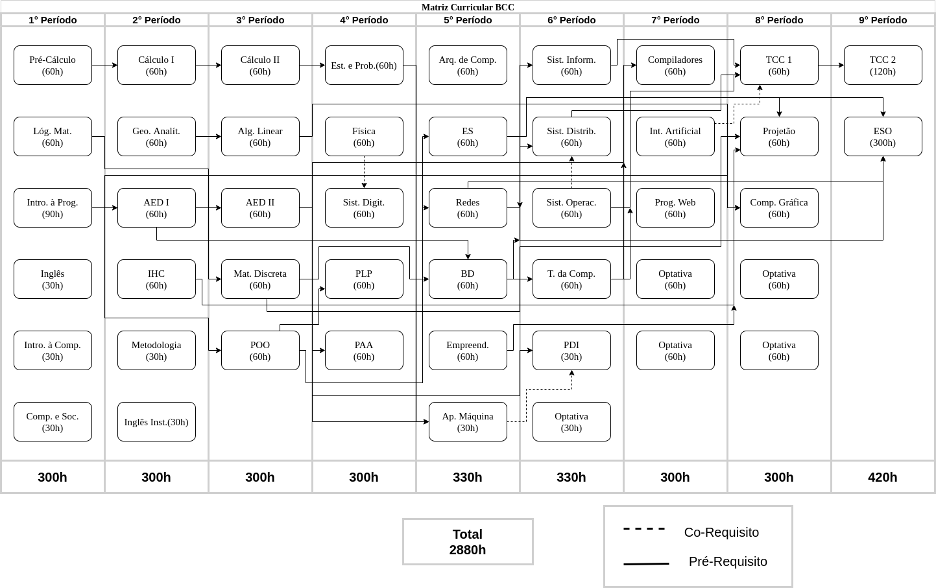
\includegraphics[width=\textwidth]{images/matriz_curricular_v3.png}
\end{figure}

\section{Quadro de Equivalência}

Diante da necessidade de adequar o perfil curricular do curso de Bacharelado em Ciência da Computação, os alunos que ingressarão no Curso a partir do semestre letivo de 2021.1 deverão compulsoriamente seguir a nova Matriz Curricular. Já os alunos que ingressaram em períodos anteriores ao semestre supracitado poderão, desde que atendam aos critérios definidos pelo Colegiado de Coordenação Didática - CCD do Curso, optar por seguir a antiga matriz curricular ou fazer a transição para a nova, buscando a equivalência de disciplinas entre as duas matrizes, conforme se mostra os Quadros 8 e 9. 

\begin{center}
  
  \begin{tiny}
    \begin{longtable}{p{6.5cm}cp{6.5cm}c}
      \caption{\label{quadro:disciplinas-obrigatorias-equivalentes}Disciplinas Obrigatórias Equivalentes.}\\
    \toprule
    \textbf{Matriz Antiga} & \textbf{CH} & \textbf{Matriz Nova} & \textbf{CH}\\
    \midrule
    - & & PRÉ-CÁLCULO & 60 \\ \midrule
    CCMP3056 INTRODUÇÃO À COMPUTAÇÃO C & 30 & INTRODUÇÃO À CIÊNCIA DA COMPUTAÇÃO & 30 \\ \midrule
    CCMP3071 COMPUTADORES E SOCIEDADE  & 30 & COMPUTADORES E SOCIEDADE & 30 \\ \midrule
    LETR3020 INGLÊS & 30 & INGLÊS  & 30 \\ \midrule
    MATM3031 CÁLCULO PARA COMPUTAÇÃO I  & 60 & CÁLCULO I & 60 \\ \midrule
    CCMP3070 INTERAÇÃO HUMANO-COMPUTADOR  & 60 & INTERAÇÃO HUMANO COMPUTADOR & 60 \\ \midrule
    - & & INGLÊS INSTRUMENTAL & 30 \\ \midrule
    CCMP3006 ALGORITMOS E ESTRUTURA DE DADOS I  & 60 & ALGORITMOS E ESTRUTURA DE DADOS & 60 \\ \midrule
    MATM3032 CÁLCULO PARA COMPUTAÇÃO II  & 60 & CÁLCULO II & 60 \\ \midrule
    MATM3019 ÁLGEBRA LINEAR  & 60 & ÁLGEBRA LINEAR I & 60 \\ \midrule
    CCMP3059 MATEMÁTICA DISCRETA  & 60 & MATEMÁTICA DISCRETA PARA COMPUTAÇÃO & 60 \\ \midrule
    CCMP3066 BANCO DE DADOS I & 60 & BANCO DE DADOS & 60 \\ \midrule
    - & & APRENDIZAGEM DE MÁQUINA & 30 \\ \midrule
    - & & PROGRAMAÇÃO WEB & 60  \\ \midrule
    CCMP3043 RECONHECIMENTO DE PADRÕES  & 60 & PROCESSAMENTO DIGITAL DE IMAGENS & 30 \\ \midrule
    CCMP3069 PROJETO DE DESENVOLVIMENTO & 90 & PROJETO DE DESENVOLVIMENTO DE SOFTWARE & 60 \\
\bottomrule
\end{longtable}
\end{tiny}
\end{center}

É importante salientar que o estudante que optar em realizar o processo de migração de perfil curricular do curso, não poderá solicitar retorno para o perfil de origem (antigo). Como pode ser observado pelo quadro de equivalências entre componentes curriculares das diferentes matrizes, o aluno que migrar para o novo perfil curricular poderá aproveitar as disciplinas já cursadas, incluindo as disciplinas optativas de acordo com o Quadro 9 abaixo.

\begin{center}
  
  \begin{tiny}
    \begin{longtable}{p{2cm}p{5.4cm}cp{5.4cm}c}
      \caption{\label{quadro:disciplinas-optativas-equivalentes}Disciplinas Optativas Equivalentes.}\\
    \toprule
    \textbf{Área} & \textbf{Matriz Antiga} & \textbf{CH} & \textbf{Matriz Nova} & \textbf{CH}\\
    \midrule
  Banco de Dados & - & & ADMINISTRAÇÃO DE BANCO DE DADOS & 60 \\ \cline{2-5}
    & CCMP3091 INTEGRAÇÃO DE DADOS E DATA WAREHOUSE & 60 & INTEGRAÇÃO DE DADOS E DATA WAREHOUSE & 60 \\ \cline{2-5}
    & - & & MINERAÇÃO DE DADOS & 60 \\ \cline{2-5}
    & - & & MODELAGEM CONCEITUAL DE DADOS & 60 \\ \cline{2-5}
    & - & & SISTEMAS DE INFORMAÇÃO GEOGRÁFICAS & 60 \\ \cline{2-5}
    & UAG00169 TÓPICOS ESPECIAIS EM BANCO DE DADOS & 60 & TÓPICOS ESPECIAIS EM BANCO DE DADOS & 60 \\ \midrule
  Engenharia da Computação & UAG00304 AVALIAÇÃO DE DESEMPENHO DE SISTEMAS & 60 & AVALIAÇÃO DE DESEMPENHO DE SISTEMAS & 60 \\ \cline{2-5}
    & - & & PROJETO DE SISTEMAS EMBARCADOS & 60 \\ \cline{2-5}
    & UAG00043 PROTOTIPAÇÃO DE CIRCUITOS DIGITAIS & 60 & PROTOTIPAÇÃO DE CIRCUITOS DIGITAIS & 60 \\ \cline{2-5}
    & - & & SISTEMAS DE TEMPO REAL & 60 \\ \midrule
  Engenharia de Software & CCMP3078 DESENVOLVIMENTO DE APLICAÇÕES MÓVEIS & 60 & DESENVOLVIMENTO DE APLICAÇÕES MÓVEIS & 60 \\ \cline{2-5}
  & CCMP3051 DESENVOLVIMENTO DISTRIBUÍDO DE SOFTWARE & 60 & DESENVOLVIMENTO DISTRIBUÍDO DE SOFTWARE & 60 \\ \cline{2-5}
    & - & & ESTIMATIVAS E MEDIÇÃO DE SOFTWARE & 60 \\ \cline{2-5}
    & - & & METODOLOGIAS ÁGEIS & 60 \\ \cline{2-5}
    & - & & PROGRAMAÇÃO ORIENTADA A ASPECTOS & 60 \\ \cline{2-5}
    & - & & PROGRAMAÇÃO ORIENTADA A OBJETOS II & 60 \\ \cline{2-5}
    & UAG00031 TESTE DE SOFTWARE & 60 & TESTE DE SOFTWARE & 60 \\ \cline{2-5}
    & - & & ESPECIFICAÇÃO FORMAL DE SOFTWARE & 60 \\ \cline{2-5}
    & - & & PROGRAMAÇÃO COMPETITIVA & 60 \\ \cline{2-5}
    & CCMP3080 TÓPICOS ESPECIAIS EM ENGENHARIA DE SOFTWARE & 60 & TÓPICOS ESPECIAIS EM ENGENHARIA DE SOFTWARE & 60 \\ \midrule
  Inteligência Computacional & - & & ALGORITMOS DE APRENDIZAGEM DE MÁQUINA & 60 \\ \cline{2-5}
    & - & & MÁQUINA DE VETORES DE SUPORTE & 60 \\ \cline{2-5}
    & - & & PROJETO EM APRENDIZAGEM DE MÁQUINA & 60 \\ \cline{2-5}
    & UAG00012 RECONHECIMENTO DE PADRÕES II & 60 & RECONHECIMENTO DE PADRÕES & 60 \\ \cline{2-5}
    & - & & REDUÇÃO DE DIMENSIONALIDADE EM APRENDIZAGEM DE MÁQUINA & 60 \\ \cline{2-5}
    & CCMP3086 TÓPICOS ESPECIAIS EM INTELIGÊNCIA ARTIFICIAL & 60 & TÓPICOS ESPECIAIS EM INTELIGÊNCIA ARTIFICIAL & 60 \\ \cline{2-5}
    & CCMP3039 REDES NEURAIS & 60 & REDES NEURAIS ARTIFICIAIS & 60 \\ \cline{2-5}
    & UAG00011 VISÃO COMPUTACIONAL & 60 & VISÃO COMPUTACIONAL & 60 \\ \midrule
  Matemática e Computação Teórica & - & & ÁLGEBRA LINEAR II & 60 \\ \cline{2-5}
    & - & & CÁLCULO III & 60 \\ \cline{2-5}
    & MATM3007 CÁLCULO PARA COMPUTAÇÃO III & 60 & CÁLCULO IV & 60 \\ \cline{2-5}
    & - & & CÁLCULO LAMBDA & 60 \\ \cline{2-5}
    & - & & INTRODUÇÃO À COMPUTAÇÃO QUÂNTICA  & 60 \\ \cline{2-5}
    & - & & OTIMIZAÇÃO COMBINATÓRIA (META-HEURÍSTICAS) & 60 \\ \cline{2-5}
    & - & & PESQUISA OPERACIONAL & 60 \\ \cline{2-5}
    & - & & REDES COMPLEXAS & 60 \\ \cline{2-5}
    & - & & TÓPICOS ESPECIAIS EM ALGORITMOS & 60 \\ \cline{2-5}
    & - & & TEORIA DOS NÚMEROS E CRIPTOGRAFIA & 60 \\ \cline{2-5}
    & - & & CRIPTOGRAFIA APLICADA & 60 \\ \cline{2-5}
    & MATM3017 CÁLCULO NUMÉRICO E COMPUTACIONAL & 60 & CÁLCULO NUMÉRICO E COMPUTACIONAL & 60 \\ \cline{2-5}
    & - & & ÁLGEBRA LINEAR COMPUTACIONAL & 60 \\ \cline{2-5}
    & - & & TÓPICOS MODELAGEM MATEMÁTICA CONTINUA & 60 \\ \midrule
  Mídia e Interação & - & & REALIDADE VIRTUAL E AUMENTADA & 60 \\ \cline{2-5}
    & CCMP3076 TÓPICOS ESPECIAIS EM PROCESSAMENTO DE SINAIS & 60 & TÓPICOS ESPECIAIS EM PROCESSAMENTO DE SINAIS & 60 \\ \cline{2-5}
    & CCMP3088 TÓPICOS ESPECIAIS EM MÍDIA E INTERAÇÃO & 60 & TÓPICOS ESPECIAIS EM MÍDIA E INTERAÇÃO & 60 \\ \midrule
  Redes e Sistemas Distribuídos & CCMP3085 GERENCIAMENTO DE REDES & 60 & GERENCIAMENTO DE REDES DE COMPUTADORES & 60 \\ \cline{2-5}
    & - & & INFRAESTRUTURA DE REDES E CABEAMENTO ESTRUTURADO & 60  \\ \cline{2-5}
    & - & & PROGRAMAÇÃO PARALELA E DISTRIBUÍDA & 60 \\ \cline{2-5}
    & - & & TÓPICOS ESPECIAIS EM REDES DE COMPUTADORES E SISTEMAS DISTRIBUÍDOS & 60 \\ \cline{2-5}
    & CCMP3079 SEGURANÇA DE REDES DE COMPUTADORES & 60 & SEGURANÇA DE REDES DE COMPUTADORES & 60 \\ \cline{2-5}
    & UAG00170 MODELAGEM DE DEPENDABILIDADE DE SISTEMAS COMPUTACIONAIS & 60 & MODELAGEM DE DEPENDABILIDADE & 60  \\ \midrule
  Tecnologia Educacional & EDUC3079 PROJETOS DE SISTEMAS EDUCACIONAIS & 60 & DESENVOLVIMENTO DE SOFTWARE EDUCACIONAL & 60 \\ \cline{2-5}
    & EDUC3048 INFORMÁTICA NA EDUCAÇÃO & 60 & INFORMÁTICA NA EDUCAÇÃO & 60 \\ \cline{2-5}
    & - & & TECNOLOGIAS ASSISTIVAS & 60 \\ \cline{2-5}
    & - & & TECNOLOGIAS, COGNIÇÃO E APRENDIZAGEM & 60 \\ \midrule
  Tecnologias da Informação & UAG00080 GESTÃO DA TECNOLOGIA DA INFORMAÇÃO & 60 & GESTÃO DA TECNOLOGIA DA INFORMAÇÃO & 60 \\ \cline{2-5}
    & CCMP3077 GESTÃO DE SERVIÇOS EM TI & 60 & GESTÃO DE SERVIÇOS EM TI & 60 \\ \cline{2-5}
    & UAG00079 GOVERNANÇA EM TECNOLOGIA DA INFORMAÇÃO & 60 & GOVERNANÇA EM TECNOLOGIA DA INFORMAÇÃO & 60 \\ \cline{2-5}
    & CCMP3083 TÓPICOS ESPECIAIS EM GESTÃO DE PROJETOS & 60 & TÓPICOS ESPECIAIS EM GESTÃO DE PROJETOS & 60 \\ \cline{2-5}
    & UAG00300 FUNDAMENTOS EM CIÊNCIA DE DADOS & 60 & FUNDAMENTOS EM CIÊNCIA DE DADOS & 60 \\ \cline{2-5}
    & UAG00024 GESTÃO DE PROCESSOS DE NEGÓCIO & 60 & GESTÃO DE PROCESSOS DE NEGÓCIO & 60 \\ \midrule
  - & EDUC3090 LÍNGUA BRASILEIRA DE SINAIS - LIBRAS L & 45 & LÍNGUA BRASILEIRA DE SINAIS - LIBRAS & 45 \\ 
\bottomrule
\end{longtable}
\end{tiny}
\end{center}

Também é importante destacar que, no momento da escolha de migração do Perfil Curricular, o discente aproveitará as Cargas Horárias oriundas de disciplinas que não apresentarem equivalência, serão contabilizadas para o Grupo de Componentes Optativos Livres.

\chapter{EMENTAS DOS COMPONENTES CURRICULARES}

As ementas\footnote{\url{https://docs.google.com/document/d/1UUd2-Y9ZuMGJe5ROmmPjHUkrayysDUXiLxDEhAbc-9o/edit?usp=sharing}} das disciplinas obrigatórias e optativas estão disponíveis no endereço abaixo para facilitar a leitura e organização deste documento, uma vez que só de ementa são quase 100 páginas.



\chapter{ESTÁGIO SUPERVISIONADO OBRIGATÓRIO}

De acordo com a Lei nº 11.788/2008, o estágio é um ``ato educativo escolar supervisionado, desenvolvido no ambiente de trabalho'' que tem o propósito de garantir o “aprendizado de competências próprias da atividade profissional e a contextualização curricular, objetivando o desenvolvimento do educando para a vida cidadã e para o trabalho”. O Estágio Supervisionado Obrigatório (ESO), fazendo parte da matriz curricular, constitui-se num espaço de aprendizagem concreta de vivência prática. O objetivo central se direciona na aplicação dos conhecimentos científicos adquiridos durante a realização do curso e a vivência profissional.

Os mecanismos de acompanhamento e de cumprimento serão estabelecidos e acompanhados pelo Coordenador do Curso em conjunto com a Comissão de Estágio Supervisionado (COE), regidos pela resolução de ESO de BCC/UAG. As atividades referentes ao estágio poderão ser encontradas na própria resolução, documento aprovado pelo Colegiado de Coordenação Didática do Curso de Bacharelado em Ciência da Computação (CCD/BCC), contendo o detalhamento das atividades permitidas, inclusive a possibilidade de equiparação de atividades para ESO, mediante aprovação do CCD/BCC, tendo em vista que a região ainda não possui um número significativo de empresas na área de Tecnologia da Informação (TI), que possam ofertar vagas e suporte adequado aos nossos alunos. Convém ressaltar que estágios relevantes para os futuros egressos deste curso envolve atividades específicas da área, devendo seguir um processo bem definido e institucionalizado. Estes, resumidamente, consistem sistematicamente nas seguintes etapas:

\begin{enumerate}
    \item Matrícula na disciplina de ESO;
    \item Solicitação do seguro junto a esta IES;
    \item Entrega do Termo de Compromisso;
    \item Realização do ESO;
    \item Escrita do Relatório Técnico do ESO;
    \item Defesa do Relatório Técnico do ESO;
    \item Avaliação do Relatório Técnico do ESO;
    \item Entrega do Relatório Técnico do ESO.
\end{enumerate}

As explanações para as etapas apresentadas estão a seguir:

\begin{enumerate}
    \item \textbf{Matrícula na disciplina de ESO} – Somente poderão se matricular na disciplina de ESO os alunos que foram aprovados nas disciplinas de Banco de Dados, Redes de Computadores e Engenharia de Software. Esta decisão leva em conta que os estagiários devem estar com aproximadamente mais da metade da carga total do curso concretizada e já possuem um grau de conhecimento adequado para estagiar na área, tornando assim o estágio melhor desenvolvido e mais bem aproveitado para um futuro vínculo empregatício.
    \item \textbf{Solicitação do seguro junto a esta IES} – Segundo a Lei nº 11.788 a contratação de seguro de vida contra acidentes pessoais em favor do estagiário é obrigatória. Como o estágio é obrigatório para obtenção do diploma no curso de Bacharelado em Ciência da Computação, Unidade Acadêmica de Garanhuns da Universidade Federal Rural de Pernambuco, o seguro fica a cargo dessa instituição de ensino.
    \item \textbf{Entrega do Termo de Compromisso} – O Termo de Compromisso de Estágio é um acordo tripartite celebrado entre o educando, a parte concedente do estágio e a instituição de ensino, prevendo as condições de adequação do estágio à proposta pedagógica do  curso, à etapa e modalidade da formação escolar  do  estudante  e ao horário e calendário escolar. O termo deve ser entregue impresso em três vias, assinadas e carimbadas pela parte concedente, pelo  Supervisor,  pelo  Orientador, pelo Estagiário e pela Instituição.
    \item \textbf{Realização do ESO} – Em hipótese alguma o estágio pode ser iniciado sem a concretização das etapas 1, 2 e 3 apresentadas anteriormente. O estágio deve ser realizado sob supervisão de alguém formado na área de TI ou que possua no mínimo dois anos de experiência na área (comprovada via diploma ou declaração) e orientado por algum professor da UFRPE (dando preferência aos professores do curso de BCC/UAG). O estagiário não deverá ultrapassar 06 (seis) horas diárias e 30 (trinta) horas semanais para as atividades do estágio, assim sendo, é preciso estipular 10 semanas para concretização das 300 horas necessárias para o ESO em BCC, considerando que este tempo deve estar dentro do prazo para finalização do período corrente e da data limite para a defesa do relatório (dadas no calendário para cada semestre letivo).
    \item \textbf{Escrita do Relatório Técnico do ESO} – Após a realização das atividades do estágio e integralização da carga horária total o estagiário deve escrever o relatório técnico do estágio, apresentando as atividades realizadas, seguindo o modelo disponibilizado pelo curso. Somente após as correções sugeridas pelo professor orientador e o aval do mesmo para defesa, o estagiário deverá imprimir uma via (espiral), que deve ser entregue para a coordenação do curso, que por sua vez, repassa para a COE, responsável por marcar a data de defesa do relatório e sugerir as melhorias.
    \item \textbf{Defesa do Relatório Técnico do ESO} – O estagiário deverá realizar uma apresentação oral do Relatório de Estágio para o professor presidente da COE. A defesa visa avaliação e composição da nota final de ESO.
    \item \textbf{Avaliação do Relatório Técnico do ESO} – A composição da nota final do ESO (média na disciplina) será dada pela avaliação realizada pelo supervisor do estagiário na empresa, através de preenchimento de formulário padrão encaminhado pela Coordenação do Curso, conceito este responsável por 25\% da nota final; pela média das notas do professor-orientador do estagiário e do presidente da COE, estes dois últimos representam os 75\% restantes para composição da nota.
    \item \textbf{Entrega do Relatório Técnico do ESO} – O acadêmico deverá apresentar, após a correção final do relatório (sugeridas pelo presidente da COE após defesa), duas cópias em CD, para ficar na Coordenação do Curso e a outra que deverá compor o acervo da Biblioteca da Unidade, devendo seguir o padrão sugerido e adotado, para mais informações o aluno deve se dirigir à biblioteca da UAG.
\end{enumerate}

Como complemento, o Estágio não obrigatório, que é uma atividade com objetivo de proporcionar ao aluno a oportunidade de aplicar seus conhecimentos acadêmicos em situações de prática profissional pode ser realizado a partir do momento que o aluno é aprovado na disciplina de Algoritmos e Estrutura de Dados, assim como não pode ultrapassar as 120 (cento e vinte) horas para aproveitamento como Atividades Complementares.

\chapter{TRABALHO DE CONCLUSÃO DE CURSO}

As disciplinas de Trabalho de Conclusão de Curso (TCC) são obrigatórias e fundamentais para desenvolvimento do discente, pois é uma oportunidade de consolidar e aprimorar os conhecimentos que adquiriu durante o curso. Tem por objetivo contribuir para a formação profissional, acadêmica e pessoal do aluno.

O Projeto do TCC complementa a formação do aluno, sendo seus resultados executados e descritos como pesquisa científica ou relatório técnico, compreendendo não somente trabalhos de pesquisa, mas trabalhos e serviços voltados para a indústria também.  Dessa maneira, a natureza do trabalho poderá ser como uma monografia, um artigo científico, um relatório técnico, entre outros. O tipo do projeto do TCC será definido entre o discente e seu orientador.

As disciplinas são ofertadas nos últimos períodos do curso e seus mecanismos de acompanhamento e de cumprimento são estabelecidos e acompanhados pelo professor responsável regidos pela resolução de TCC de BCC. A primeira disciplina possui 60 (sessenta) horas e tem o objetivo maior no entendimento do propósito, na construção e definição do projeto de TCC, onde através de aulas e acompanhamento do professor da disciplina, o discente, possa começar a executar seu trabalho e no semestre seguinte, matriculado na segunda disciplina, de 120 (cento e vinte) horas, com o projeto já adiantado, possa ter maiores chances de desenvolver seu trabalho no prazo esperado, diminuindo o risco de postergar seu curso em tanto tempo. Para cursar a disciplina de TCC 1 é necessário que o discente tenha integralizado pelo menos 50\% do curso.


\chapter{ATIVIDADES COMPLEMENTARES}

As atividades complementares têm a finalidade de propiciar saberes e habilidades que enriqueçam o processo de ensino e aprendizagem, possibilitando a ampliação dos conhecimentos didáticos, curriculares, científicos e culturais por meio de atividades realizadas nos mais diversos espaços (Unidades Acadêmicas da Universidade, ONGs, Instituições públicas e privadas, etc). Essas atividades de formação complementar abrangem as modalidades de ensino, pesquisa e extensão, bem como as suas formas de registro no histórico escolar, devidamente detalhadas na Resolução CEPE/UFRPE nº 362/2011. 

Ainda de acordo com a resolução supracitada, em seu Art. 1º, Parágrafo único, “toda atividade acadêmica complementar deverá ficar sobre a responsabilidade, de, pelo menos, um professor, devendo ser avaliada e homologada pelo Colegiado de Coordenação Didática – CCD do curso”. Neste sentido, o acompanhamento e avaliação dessas atividades estarão integrados ao planejamento do curso. O aluno deverá, obrigatoriamente, apresentar uma ou mais atividades de naturezas distintas, sejam Ensino, Pesquisa ou Extensão. O Quadro abaixo apresenta uma breve amostra de atividades complementares previstas para o Bacharelado em Ciência da Computação.

\begin{center}
  
  \begin{scriptsize}
    \begin{longtable}{p{2.5cm}p{3.5cm}p{6cm}p{2cm}}
      \caption{\label{quadro:atividades-complementares}Atividades complementares previstas para o curso.}\\
      \toprule
      \textbf{Modalidade} & \textbf{Atividade} & \textbf{Descrição} & \textbf{C.H}\\ 
        \midrule
        Formação \newline Profissional & Estágio não Obrigatório & Atividade que tem o objetivo de proporcionar ao aluno a oportunidade de aplicar seus conhecimentos acadêmicos em situações de prática profissional. & Não exceder 120 horas\\
        \addlinespace
        & Cursos de Formação Profissional Complementar & Cursos ofertados à comunidade sob a forma de Educação Continuada, objetivando a socialização do conhecimento acadêmico, potencializando o processo de interação universidade-sociedade. & \\
        & Pesquisa de Iniciação Científica & Conjunto de atividades ligadas a programas e projetos de pesquisa desenvolvidos pelo Aluno, sob orientação do Docente. & \\
        \addlinespace
        & Realização de Visita técnica & Visitas a lugares de interesse para a área de formação que complementem o conteúdo das disciplinas, relacionando teoria e prática. & \\
        \midrule
        Extensão Universitária e Aperfeiçoamento & Projetos de Extensão & Ações processuais, de caráter educativo, cultural, artístico, científico e/ou tecnológico, que envolvem Docentes, Alunos e Técnico-administrativos, e que são desenvolvidas junto à comunidade, mediante ações sistematizadas. & Não exceder 120 horas \\
        \addlinespace
        & Participação em Eventos de Extensão (internos e externos) & Participação em Congressos, Seminários, Jornadas e similares, que possuam o propósito de produzir, sistematizar, divulgar e intercambiar conhecimentos, tecnologias e bens culturais. & \\
        \addlinespace
        & Apresentação de Trabalhos em Eventos & Apresentação oral de trabalhos acadêmicos em Congressos, Seminários, Jornadas e similares. & \\ \addlinespace
        & Publicação científica & Divulgação dos resultados da investigação através da produção de artigos. & \\ \addlinespace
        & Prestação de serviços à comunidade & Participação em atividades que possibilitem a transferência à comunidade do conhecimento gerado no âmbito do curso. & \\ \midrule
        Experiência de Ensino & Monitoria & Ação de cooperação dos corpos discente e docente nas atividades de ensino, pesquisa e extensão efetuadas em trabalhos de laboratório, biblioteca, de campo e outras compatíveis com seu nível de conhecimento e experiência nas disciplinas e desenvolver habilidades que favoreçam o Aluno na iniciação à docência. & Não exceder 120 horas \\ \addlinespace
        & Participação em Projetos de Ensino & Participação, em ações devidamente reconhecidas pela Universidade de acordo com a legislação vigente, que tem por objetivo estimular e apoiar as ações de Ensino, não curriculares, com caráter temporário, complementar e/ou de aprofundamento, que visam à melhoria do processo de ensino aprendizagem dos cursos de Graduação ofertados na UFAPE e que tenham como público alvo membros internos da comunidade universitária. São exemplos de projetos de ensino: cursos, grupos de estudo e eventos. & \\ \addlinespace
        Políticas & Representação discente em comissões e comitês
        Participação em órgãos colegiados da UFRPE. & Participação em órgãos colegiados da UFRPE.& \\ \addlinespace
        Empreendedorismo e Inovação & Participação em Empresas Júnior, incubadoras ou outros mecanismos & Participação, desenvolvimento e execução de projetos. & \\ \addlinespace
        & Desenvolvimento de protótipo ou produto & Produção de materiais. & \\
      \bottomrule
    \end{longtable}
    \nota[Fonte]{Adaptado dos Referenciais da SBC, 2017 e da Resolução CEPE/UFRPE nº 362/2011.}
  \end{scriptsize}      
\end{center}

A carga horária total das atividades complementares para o curso de Ciência da Computação é de 320h. Esta será considerada apenas mediante o requerimento protocolado à Coordenação do Curso e acompanhado da documentação comprobatória.


\chapter{CRITÉRIOS DE APROVEITAMENTO DE ESTUDOS}

O aproveitamento de estudos corresponde à dispensa de cumprimento de disciplinas regulares do curso, quando a mesma ou uma equivalente em conteúdo e carga horária são cumpridas em outro curso superior, seja no âmbito da UFRPE ou de outra instituição.

Na UFRPE, a dispensa de disciplinas encontra-se normatizada pela Resolução CEPE/UFRPE nº 442/2006. Para que sejam creditadas, as disciplinas cursadas deverão:

\begin{enumerate}[label=(\alph*)]
  \item ser equivalentes em, pelo menos, 80\% (oitenta por cento) do conteúdo programático às correspondentes disciplinas que serão dispensadas; 	
  \item ter carga horária igual ou superior àquela das disciplinas a serem dispensadas; 	
  \item ser oferecidas regularmente pela Instituição onde foram cursadas como integrantes do currículo de um curso devidamente reconhecido.
\end{enumerate}

O pedido de dispensa da disciplina será dirigido ao coordenador do curso do solicitante, através de requerimento, acompanhado de histórico escolar ou declaração e do programa da disciplina a ser creditada. No requerimento deverão ficar esclarecidos códigos e denominações da disciplina a ser creditada e da disciplina a ser dispensada. Os pedidos de dispensa serão analisados por representantes dos cursos e homologados pelo CCD.

Este último terá a incumbência de realizar a dispensa das disciplinas não cursadas na UFRPE. Em se tratando de disciplina cursada na UFRPE, a dispensa será analisada e decidida diretamente pelo Coordenador, que informará ao CCD das dispensas, sendo obrigatório o registro em ata.

Existe a possibilidade de abreviação do tempo de formação para os alunos que demonstrem extraordinário aproveitamento nos estudos, como previsto na Lei nº 9.394/96, no Art. 47, § 2º. Este aparato legal ainda está em processo de regulamentação pela UFRPE com base na Resolução CFE nº 1/94 e no parecer CES/CNE n° 247/99.



\chapter{METODOLOGIA E AVALIAÇÃO}

As discussões sobre os processos de formação no Ensino Superior têm destacado a relação entre conhecimento e ensino no contexto de uma transição paradigmática das Ciências que, dentre outros aspectos, se caracteriza pela emergência de sistemas de conhecimento abertos e não dicotômicos (SANTOS, 1988). Segundo Cunha (2005, p. 13), o “paradigma emergente” nas Ciências situa os professores do magistério superior diante de novos desafios, a saber:

\begin{enumerate}[label=(\alph*)]
    \item Enfoque no conhecimento a partir da historicidade de sua produção e de sua provisoriedade e relatividade;
    \item Estímulo à análise, à capacidade de composição de dados, informações, argumentos e ideias;
    \item Valorização da curiosidade, do questionamento e da incerteza;
    \item Percepção do conhecimento como interdisciplinar, estabelecendo relações e atribuição de significados em função dos objetivos sociais e acadêmicos;
    \item Valorização da pesquisa como um instrumento do ensino e a extensão como ponto de partida e chegada da apreensão da realidade;
    \item Valorização das habilidades sócio-intelectuais tanto quanto os conteúdos.
\end{enumerate}

Neste contexto, a docência assume um novo papel deslocando-se do modelo onde figurava como fonte da informação para uma posição de mediação entre o aluno e o seu objeto de conhecimento. O destaque dado à importância da autonomia do estudante em seu processo de desenvolvimento intelectual, social e afetivo põe em relevo o protagonismo do processo de ensino e aprendizagem na consecução dos objetivos do curso (seção 4), considerando o perfil do egresso (seção 5) e as respectivas competências e habilidades esperadas de um Bacharel em Ciência da Computação. Diante disso, este projeto orienta-se por determinadas concepções teórico-metodológicas, tendo em vista possibilitar a execução do escopo almejado.

\section{Concepção de ensino e aprendizagem}

O ensino e a aprendizagem são compreendidos como elementos constituintes de um mesmo processo de construção do conhecimento em que o aluno e seu objeto de estudo estão em contínua relação mediados pela ação do professor (ANASTASIOU; ALVES, 2015). Isso significa que o ensino não corresponde a uma transmissão de informações, mas assume um caráter dialógico, problematizador e contextualizador do próprio objeto de conhecimento (FREIRE, 2005b). O professor age de modo a estimular a aprendizagem, valorizando os conhecimentos prévios dos alunos, proporcionando-lhes experiências de pesquisa, interação social e expressão de saberes, práticas, atitudes e valores, ao mesmo tempo em que avalia permanentemente o seu desenvolvimento.

Nessa concepção, os conteúdos da aprendizagem não se apresentam isolados de sua dimensão epistemológica, social ou política. Além disso, tais conteúdos são abrangentes, incluindo fatos, conceitos, procedimentos e atitudes (ZABALA, 1998). O professor deve, então, fomentar, junto aos seus alunos, momentos que estimulem a apreensão da complexidade inerente ao objeto de estudo por meio da problematização. O processo de ensino-aprendizagem numa perspectiva ativa, e não mecânica ou “bancária” (FREIRE, 2005a), coloca o aluno como protagonista de seu desenvolvimento intelectual, social e afetivo ao mobilizar seu potencial para responder aos desafios postos pelos novos saberes (BERBEL, 2011). Tal postura favorece uma “aprendizagem significativa” em que os novos conhecimentos interagem de maneira substantiva, ou seja, não literal, com os conhecimentos já construídos pelo aluno. Neste sentido, trata-se de uma aprendizagem não arbitrária, pois se apoia nos conhecimentos prévios dos alunos tornando-os mais ricos ou dotados de novos significados, de modo a estimular a criatividade e autonomia (MOREIRA, 2010).

Compreendido desta forma, o processo de ensino-aprendizagem possibilita considerar a tríade professor-conhecimento-aluno a partir de novas perspectivas. Por exemplo, as concepções de espaço e tempo do ensinar e do aprender distanciam-se da tradicional clivagem entre ensino presencial e virtual em prol de uma concepção híbrida possibilitando, assim, o uso planejado das mais variadas tecnologias digitais aliadas a uma interação entre o aluno e o grupo-classe.

\section{As Tecnologias da Informação e Comunicação – TICs aplicadas ao ensino e a aprendizagem}

O ensino híbrido representa uma quebra de paradigmas em direção a uma proposta de inovação mais alinhada com os avanços tecnológicos de uma sociedade pós-moderna. Pensar o ensino híbrido, portanto, significa organizar estratégias metodológicas utilizando atividades presenciais e a distância em plataformas on-line, empregando TICs, e off-line, nos momentos de interação com colegas e/ou com o professor/tutor. Segundo Christensen, Horn e Staker (2013), no ensino híbrido, o aluno aprende:

\begin{citacao}
    “Pelo menos em parte por meio do ensino online, com algum elemento de controle do estudante sobre o tempo, local, caminho e/ou ritmo de estudo e, pelo menos em parte, em uma localidade física supervisionada, fora de sua residência. As modalidades ao longo do caminho de aprendizado de cada estudante em um curso ou matéria são conectadas para oferecer uma experiência de educação integrada”.
\end{citacao}

Nessa perspectiva, seja presencialmente ou à distância, o estudante compartilha de espaços interativos e integrativos de aprendizagem. São exemplos de uma abordagem híbrida do ensino (BACICH; NETO; TREVISANI, 2015):

\noindent \textbf{Sala de aula invertida}: o aluno estuda a teoria em casa utilizando-se de plataforma on-line; o tempo e o espaço da sala de aula são utilizados para discussões e realização de atividades. Os assuntos são disponibilizados previamente pelo professor no Ambiente Virtual de Aprendizagem – AVA. No momento da aula, os alunos compartilham com o professor suas observações a respeito do material estudado previamente e, seguindo, um plano de trabalho, desenvolvem atividades relacionadas com a teoria, com uso das mais variadas estratégias: rotação por estações, laboratório rotacional, seminários, estudos de caso, etc.

\noindent \textbf{Rotação por estações}: os alunos são divididos em grupos (estações), cada qual realizando uma determinada tarefa, tendo em vista os objetivos definidos no plano de aula. Um dos grupos estará, necessariamente, desenvolvendo alguma atividade de forma on-line. Após transcorrer um determinado período, os alunos trocam de grupo, de modo a trabalhar em uma tarefa diferente da sua. Este revezamento continua até que todos os estudantes tenham passado por todos os grupos. 

Ainda que as atividades realizadas em cada grupo sejam independentes, no final, elas funcionam de forma integrada, possibilitando, assim, uma compreensão de conjunto do objeto estudado.

\noindent \textbf{Laboratório rotacional}: é semelhante ao modelo da rotação por estações, mas, neste caso, o revezamento envolve o deslocamento para um laboratório de informática onde cada aluno executará, individualmente, a atividade, sob a mediação de um tutor.

\noindent \textbf{Rotação individual}: o aluno trabalha sozinho devendo cumprir uma lista de temas ou atividades planejadas pelo professor. O tempo que o aluno terá para desenvolver suas tarefas é livre, pois varia de acordo com as suas necessidades.

Cabe ao professor, portanto, não só conhecer diversas ferramentas \textit{on-line} disponíveis para a aprendizagem como, também, estabelecer a correta utilização destes instrumentos em função dos objetivos pedagógicos a serem atingidos. Diante disso, o uso do AVA se apresenta como elemento intrínseco ao planejamento de ensino. Compreendido como um sistema computacional destinado ao suporte de atividades mediadas pelas TIC's, o AVA permite ``integrar múltiplas mídias, linguagens e recursos'', além do ``gerenciamento de banco de dados'', ampliando ``a intercomunicação e a socialização de experiências na construção de aprendizagens colaborativas'' (SILVA, 2011, p. 2).
	
O AVA pode ser utilizado tanto para formação exclusivamente \textit{on-line} quanto presencial. Nele, professores e alunos têm acesso a diversas ferramentas, tais como: e-mails, blogs, fóruns de discussão, chats, glossários interativos, quiz, \textit{webquests}, \textit{wikis}, vídeos, etc. Caracterizado pela interatividade, hipertextualidade e conectividade, o AVA possibilita a ``flexibilidade de navegação'' e formas ``síncronas e assíncronas de comunicação'' oferecendo aos alunos, ``a oportunidade de definirem seus próprios caminhos de acesso às informações, afastando-se de modelos massivos de ensino e garantindo aprendizagens personalizadas'' (SILVA, 2011, p. 5).

\section{Estratégias metodológicas}

O ensino de computação com uso das TIC's se beneficia das inúmeras possibilidades que universos digitais e comunicacionais oferecem, possibilitando aprendizagens em rede, na perspectiva do espraiamento de espaços, tempos e itinerários formativos. Uma abordagem híbrida do processo de ensino-aprendizagem não implica a exclusão de estratégias de ensino mais tradicionais, uma vez que o fenômeno educativo é complexo e dinâmico. Novas estratégias podem surgir decorrentes da organização do trabalho docente. O Quadro 16 apresenta alguns exemplos de estratégias metodológicas, dentre outras tantas opções existentes.

\begin{center}
    
    \begin{scriptsize}
        \begin{longtable}{p{4.5cm}p{10cm}}
            \caption{\label{quadro:proposicoes-estrategias-metodologicas}Proposições de estratégias metodológicas.}\\
      \toprule
      \textbf{Estratégia metodológica} & \textbf{Descrição}\\ 
        \midrule
        Aula expositiva & Consiste em uma apresentação oral visando iniciar um tema de estudo, “fazer uma síntese do assunto estudado procurando reunir os pontos mais significativos, [ou] estabelecer comunicações que tragam atualidade ao tema ou explicações necessárias” (MASETTO, 2012). A aula expositiva não objetiva a reprodução contínua de informações presentes em livros e artigos, ela procura motivar os alunos ao estudo de um determinado tema, oferecer uma síntese, destacar conceitos-chave ou elucidar pontos complexos da matéria.\\ \midrule
        Seminário & Contribui para o desenvolvimento da prática de pesquisa e discussão de argumentos. O seminário compõe-se de uma mesa-redonda composta por representantes discentes de diversos grupos que, por sua vez, pesquisaram um tema específico. Com a mediação do professor, os resultados dessas pesquisas são debatidos à luz de um tema geral proposto para o encontro. “O resultado dessa mesa-redonda pode ser um texto produzido pelos alunos com a coordenação do professor sobre o novo tema” (MASETTO, 2012) A prática do seminário está muito associada ao “ensino com pesquisa”. \\ \midrule
        Estudo de caso & Utiliza-se de uma situação real do universo profissional do graduando, de modo a relacionar teoria e prática, desenvolvendo habilidades específicas no trato com problemas concretos. “O que se espera com o uso dos casos é que o estudante se coloque no lugar da pessoa a quem cabe tomar a decisão ou resolver o problema. Apesar de terem sido retirados de situações reais para as quais muitas vezes houve uma decisão conhecida, esta não é apresentada, restando aos estudantes a tarefa de determinar qual a solução mais adequada. Os casos são utilizados como catalisadores da discussão” (GIL, 2006). \\ \midrule
        Textos, Imagens e Documentos & Consiste na análise de trechos selecionados de livros ou artigos, bem como de imagens ou quaisquer documentos relevantes para um determinado tema de estudo. Não se trata de ler o conteúdo da matéria em sala de aula, mas sim de explorar fontes relacionadas à discussão proposta pelo professor. Tal estratégia contribui para solidificar a habilidade de interpretação com base em aspectos intrínsecos e extrínsecos à fonte analisada. \\ \midrule
        Discussões & Com base em Gil (2006), pode-se dizer que a prática da discussão no processo de ensino-aprendizagem reveste-se de grande importância pedagógica, na medida em que:

        \begin{enumerate}[midsep]
            \item favorece uma reflexão acerca do que foi aprendido;
            \item oportuniza aos estudantes o espaço para formularem princípios com suas próprias palavras;
            \item ajuda os discentes a identificaram problemas apresentados em leituras e preleções;
            \item promove o envolvimento entre os alunos e destes com o professor;
            \item estimula o pensar crítico; 	
            \item postula o respeito a ideias divergentes.
        \end{enumerate}

        A discussão pode ocorrer utilizando-se das mais variadas técnicas: “Brainstorming”, “Grupos de Cochicho”, “Phillips 66”, “Painel Integrado”, “GVGO”, “Grupo de Oposição”, etc.\\ \midrule
        Visitas Técnicas & Constituem uma oportunidade de contato com o ambiente profissional do futuro bacharel. A visita deve ter bem claro seus objetivos e estar relacionada aos temas que estão sendo estudados. Os estudantes seguem um roteiro de observações e registram tudo o que for relevante ao propósito do trabalho. Após a visita, os alunos elaboram um relatório para discuti-lo durante a aula com os demais colegas e com o professor. “Neste debate é importante trazer as questões teóricas buscando a interação entre teoria e prática” (MASETTO, 2012, p. 146).\\
      \bottomrule
\end{longtable}
\end{scriptsize}      
\end{center}

O professor deverá, por meio do planejamento e contínua reflexão sobre a prática, definir as estratégias metodológicas que melhor se adequem aos objetivos propostos e às necessidades de seus alunos. Segundo Gil (2006), o planejamento de ensino se configura como condição essencial para o êxito do trabalho do professor, pois “à medida que as ações docentes são planejadas, evita-se a improvisação, garante-se maior probabilidade de alcance dos objetivos, obtêm-se maior segurança na direção do ensino e, também, maior economia de tempo e de energia”.
	
As estratégias metodológicas, por si mesmas, não são garantia de eficácia do ensino. Elas só concorrerão para uma aprendizagem significativa na medida em que estiverem pautadas por um planejamento que leve em consideração à heterogeneidade dos sujeitos em formação.

\section{Acessibilidade pedagógica}

Um aspecto a ser observado pelos docentes no processo de ensino-aprendizagem é o da inclusão da pessoa com deficiência e da acessibilidade. A inclusão pode ser compreendida como um movimento social, político e educacional que vem defender o direito de todos os indivíduos participarem, de uma forma consciente e responsável, na sociedade de que fazem parte, e de serem aceitos e respeitados naquilo que os diferencia dos outros. Neste contexto, a acessibilidade, como uma das dimensões da inclusão, apresenta-se como possibilidade e:

\begin{citacao}
    “Condição de alcance para utilização, com segurança e autonomia, de espaços, mobiliários, equipamentos urbanos, edificações, transportes, informação e comunicação, inclusive seus sistemas e tecnologias, bem como de outros serviços e instalações abertos ao público, de uso público ou privados de uso coletivo, tanto na zona urbana como na rural, por pessoa com deficiência ou com mobilidade reduzida”. (LBI, nº 13.146/2015).
\end{citacao}

A acessibilidade engloba diversas dimensões, a saber: atitudinal, comunicacional, digital, instrumental, programática, arquitetônica e metodológica. Esta última, de acordo com Sassaki (2013), diz respeito à ausência de barreiras nas metodologias e técnicas de estudo. Assim sendo, ela está diretamente relacionada à prática docente, ou seja, a forma como os professores concebem conhecimento, aprendizagem, avaliação e inclusão educacional irá determinar, ou não, a remoção das barreiras pedagógicas.

Buscando viabilizar o processo de ensino e aprendizagem dos estudantes com deficiência, serão realizadas adaptações curriculares dos conteúdos programáticos, flexibilizados os prazos para produção e entrega de atividades, bem como adotados processos avaliativos e recursos específicos que atendam às necessidades de cada estudante (pranchas de comunicação, texto impresso e ampliado, softwares ampliadores de comunicação alternativa, leitores de tela, entre outros recursos de tecnologia presentes na instituição).

Os professores contarão com o apoio do Núcleo de Acessibilidade - NACES, através do serviço de Atendimento Educacional Especializado, assim como de tecnologias assistivas disponibilizadas nos Laboratórios de Acessibilidade - LA que se encontram em fase de implantação na Sede e nas Unidades Acadêmicas. Os estudantes com deficiência poderão, ainda, dispor de atendimento psicológico por meio do Setor de Saúde da UAG.

\section{Projetos interdisciplinares}

A interdisciplinaridade, segundo Japiassú (1976, p. 74), pode ser caracterizada pela “intensidade das trocas entre os especialistas e pelo grau de interação real das disciplinas no interior de um mesmo projeto de pesquisa”. Essa interação envolve não só aspectos metodológicos, mas também a adoção de uma postura dialógica frente a saberes e sujeitos. As estratégias de ensino interdisciplinares contribuem para a construção do que Morin (2002) denomina de "conhecimento pertinente”, isto é, uma visão de conjunto, no qual o contexto local e o global estão em relação de reciprocidade.
	
Partindo desse entendimento, o curso de Ciência da Computação oportuniza aos alunos o desenvolvimento de projetos interdisciplinares ao longo de sua formação. Para tanto, os professores vivenciam momentos coletivos de formação pedagógica e planejamento, elegendo, neste último caso, os objetivos dos projetos, as disciplinas que estarão envolvidas, os recursos necessários, às etapas de desenvolvimento e a avaliação.

Nos projetos interdisciplinares, o curso também adota a PBL como uma de suas metodologias de ensino. A PBL tem por base a investigação como ponto de partida para a aquisição e integração de novos conhecimentos. Ela valoriza os conhecimentos prévios dos alunos, favorecendo a capacidade crítica de análise e construção de soluções para as situações-problema (BARROWS, 1986). Além das competências técnicas específicas exigidas por cada disciplina, a realização dos projetos contribuirá para desenvolver um conjunto de competências transversais, tais como a capacidade de comunicação, liderança, gestão de conflitos, tomada de decisão e gestão do tempo, dentre outras (CABRAL-CARDOSO; ESTEVÃO; SILVA, 2006), conforme a figura abaixo:

\begin{figure}[!htb]
    \centering
    \caption{\label{fig:competencias-pbl}Competências trabalhadas na PBL.}
    
    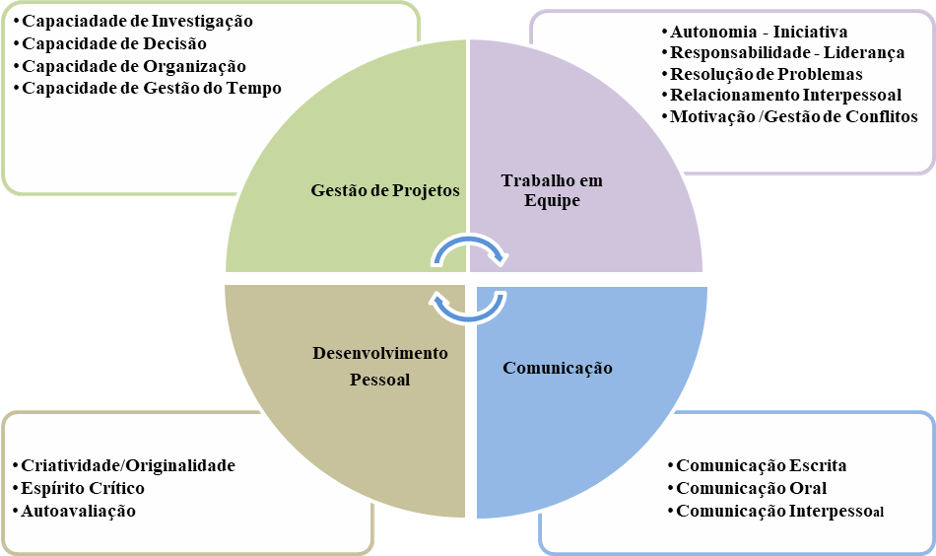
\includegraphics[width=\textwidth]{images/competencias_pbl.png}
  \end{figure}

Na PBL, a avaliação não se apresenta exclusivamente como um mecanismo de atribuição de nota, mas busca o feedback do aluno no que diz respeito às suas dificuldades no processo de aprendizagem (DELISLE, 2000; CARVALHO, 2009). Neste sentido, cada uma das etapas de desenvolvimento dos projetos será acompanhada de forma sistemática pelos professores.	
A próxima seção apresenta uma discussão mais ampla sobre a concepção de avaliação no âmbito deste projeto.

14.6. Avaliação do ensino e da aprendizagem

No decorrer da história da educação, foi atribuída à avaliação significados bastante diversos, resultantes das diferentes formas de conceber a relação entre ensino e aprendizagem. Apesar da pluralidade de definições e enfoques dados à avaliação, os estudos contemporâneos demonstram que avaliar para excluir ou meramente classificar a aprendizagem dos alunos está aquém do que de fato seriam as funções da avaliação (LUCKESI, 2003). Além disso, as práticas avaliativas exercidas pelos professores não podem ser entendidas em si mesmas, já que elas têm relação com as finalidades sociais mais amplas da educação.
	
Balizando-se por estas acepções, a avaliação no curso de Bacharelado em Ciência de Computação apresentará informações, em momentos diferenciados, acerca dos percursos de aprendizagens dos alunos e, também, sobre as práticas de ensino dos docentes (com vistas ao replanejamento do trabalho pedagógico). Esta compreensão é resultante do entendimento de que a avaliação atua como mediadora tanto do ensino quanto da aprendizagem (HOFFMAN, 2005). Assim, como uma atividade inerente à ação educativa, a avaliação:

\begin{enumerate}[label=(\alph*)]
    \item Estará	diretamente vinculada aos objetivos e às disciplinas do curso; 
    \item Ocorrerá de forma contínua, democrática, dinâmica, inclusiva, sistemática e intencional;
    \item Considerará as especificidades de cada componente curricular;
    \item Será pautada por critérios e instrumentos bem definidos;
    \item Servirá de informação para a melhoria não só do resultado, mas do processo de formação dos alunos.
    \item Levará	em conta as potencialidades dos estudantes considerando o real e não apenas o ideal.
\end{enumerate}

Evidentemente, cada tipo de conteúdo (conceitual, factual, procedimental e atitudinal) demanda formas específicas de ensinar e, por conseguinte, de avaliar. Conclui-se, portanto, a necessidade de os professores fazerem uso de variados instrumentos avaliativos apresentando, estes últimos, qualidade satisfatória, sob o risco de qualificar de forma inadequada os processos formativos dos discentes (SILVA, 2003). Portanto, os instrumentos escolhidos para atingir os objetivos pretendidos estarão adequados:

\begin{enumerate}[label=(\alph*)]
    \item Às competências e habilidades que estão sendo avaliadas;
    \item Aos conteúdos propostos e ministrados pelo docente; 
    \item À linguagem, de modo que o aluno possa compreender exatamente o que está sendo solicitado dele; 
    \item Ao processo de aprendizagem dos discentes.     
\end{enumerate}

No curso de Ciência da Computação, a avaliação ocorrerá, sistematicamente, durante todo o processo de ensino-aprendizagem, e não somente ao final de cada semestre. Por isso, será importante que não seja adotado, com exclusividade, uma única modalidade avaliativa (diagnóstica, processual ou somativa), mas que estas ocorram de forma articulada. Em determinados momentos poderão, ainda, ser estimuladas práticas de autoavaliação das aprendizagens, sendo estas condições didáticas importantes para a construção da autonomia dos estudantes.

QUADRO AQUI

O \textit{feedback} das avaliações constitui um aspecto fundamental no processo de acompanhamento do desenvolvimento do aluno, tendo em vista a construção, reconstrução e apropriação do conhecimento. Diante disso, também será assegurado aos estudantes o conhecimento dos pressupostos avaliativos que regem o curso de Bacharelado em Ciência de Computação, conforme o Parecer CNE/CES nº 236/2009.
	
A Universidade, por meio da Resolução CEPE/UFRPE nº494/2010, estabeleceu os procedimentos normativos no que tange ao registro das avaliações no âmbito do ensino da graduação. De acordo com este dispositivo, em cada disciplina serão realizadas três (3) verificações de aprendizagem e um exame final. Cada verificação de aprendizagem poderá ser feita através de uma única prova escrita ou de quaisquer outros instrumentos de avaliação, dependendo da natureza da disciplina e da orientação docente. As atividades avaliativas, além do seu caráter formativo e processual, terão, igualmente, um caráter cumulativo. Neste caso, “para efeito do cômputo do aproveitamento do aluno, nas verificações de aprendizagem e no exame final, serão atribuídas notas variando de zero (0) a dez (10), permitindo-se seu fracionamento em centésimos” (Art. 5º, §1º).

A frequência às aulas e demais atividades escolares será obrigatória, conside\-ran\-do-se reprovado na disciplina o aluno que não comparecer ao mínimo de 75\% (setenta e cinco por cento) das aulas ministradas (teóricas e práticas), ressalvados os casos previstos em lei (Art. 8º, Inciso I). Para fins de aprovação, além do mínimo de frequência exigido, o aluno deverá possuir média final igual ou superior a sete (7,0) em duas verificações da aprendizagem ou média final superior a cinco (5) entre a média de duas verificações de aprendizagem e a nota do exame final (Art. 7º, incisos I e II).

As disciplinas ministradas na modalidade EAD, terão suas avaliações na forma presencial, de acordo com a Portaria MEC nº 1.134/2016.

\section{Acessibilidade nos processos avaliativos}

Ainda no tocante à avaliação pedagógica, o curso de Bacharelado em Ciência da Computação encontra-se balizado, também, pela Política Nacional para Educação Especial na perspectiva da Educação Inclusiva (BRASIL, 2008). Nesta, a avaliação configura “uma ação pedagógica processual e formativa que analisa o desempenho do aluno em relação ao seu progresso individual, prevalecendo [\ldots] os aspectos qualitativos que indiquem as intervenções pedagógicas do professor”.

Com esse entendimento, o princípio da \textit{inclusão} norteará o processo de ensino e aprendizagem, garantindo que os professores, ao realizarem suas avaliações, promovam adaptações em função das necessidades educacionais especiais dos estudantes. Para os alunos que são considerados público-alvo da educação inclusiva (pessoas com deficiência, transtornos globais do desenvolvimento e com altas habilidades/superdotação), os docentes utilizarão, dentre outras estratégias, as seguintes adaptações avaliativas: \textit{dilatação de tempo de avaliação, apresentações de trabalhos em dupla, em equipes ou individual, prova oral, individualizada, sinalizada, ampliada, em Braile, em Libras, com recurso de tecnologias assistivas, permanência de profissional de apoio ou intérprete de Libras em sala e etc}.

É possível, assim, afirmar que, ao se adaptar uma avaliação ou uma estratégia didática, objetiva-se assegurar a equiparação de oportunidades, uma vez que todos os alunos são capazes de aprender, independente da sua idade cronológica, das suas limitações e de suas especificidades. Desse modo, o respeito à individualidade e ao tempo de cada um constitui um princípio fundamental para uma educação inclusiva.

\section{Integração entre as atividades de ensino, pesquisa e extensão}

Ensino, Pesquisa e Extensão constituem as áreas de atuação da Universidade e, conforme o disposto na Constituição Federal, em seu Art. 207, devem ser indissociáveis entre si. Neste sentido, o Programa de Educação Tutorial – PET, financiado pelo MEC, possibilita que os estudantes tenham uma ampla formação, na medida em que propõe o desenvolvimento de atividades que envolvem, de forma articulada, ensino, pesquisa e extensão. São alguns objetivos do Programa:

\begin{enumerate}[label=(\alph*)]
    \item Desenvolver atividades acadêmicas em padrões de qualidade de excelência, mediante grupos 	de aprendizagem tutorial de natureza coletiva e interdisciplinar;
    \item Contribuir para a elevação da qualidade da formação acadêmica dos alunos de graduação;
    \item Formular novas estratégias de	desenvolvimento e modernização do ensino superior no país;
    \item Introduzir novas práticas pedagógicas na graduação; 
    \item Contribuir com a política de diversidade na IES, por meio de ações afirmativas em defesa da equidade socioeconômica, étnico-racial e de gênero.
\end{enumerate}

	Na UFRPE existem 18 grupos PET organizados em quatro eixos (Original, Conexões Saberes, Engenharias e Interdisciplinar). No que tange à prática iniciação à pesquisa, esta é incentivada por meio do Programa Institucional de Bolsas de Iniciação Científica – PIBIC, financiado pelo Conselho Nacional de Desenvolvimento Científico e Tecnológico – CNPq, pela Fundação de Amparo à Ciência e Tecnologia do Estado de Pernambuco – FACEPE e pela própria Universidade. Dentre os objetivos do PIBIC, está o de:

\begin{enumerate}[label=(\alph*)]
    \item Despertar a vocação científica e incentivar novos talentos entre estudantes de graduação;
    \item Estimular uma maior articulação entre a graduação e pós-graduação;
    \item Estimular pesquisadores produtivos a envolverem alunos de graduação nas atividades científica, tecnológica e artístico-cultural;
    \item Proporcionar ao bolsista, orientado por pesquisador qualificado, a aprendizagem de técnicas e métodos de pesquisa, bem como estimular o desenvolvimento do pensar cientificamente e da criatividade, decorrentes das condições criadas pelo confronto direto com os  problemas de pesquisa;
    \item Ampliar o acesso e a integração do estudante à cultura científica.
\end{enumerate}

Outro importante exemplo é o Programa de Iniciação Científica – PIC, por meio do qual são concedidas cotas de orientação aos docentes/pesquisadores sem concessão de bolsas aos discentes. Trata-se de uma ação que amplia a formação de discentes/pesquisadores na instituição compartilhando dos objetivos do PIBIC. Já o Programa Institucional de Bolsas de Iniciação em Desenvolvimento Tecnológico e Inovação – PIBITI, financiado pelo CNPq, objetiva contribuir para a:

\begin{enumerate}[label=(\alph*)]
    \item Formação e inserção de estudantes em atividades de pesquisa,  desenvolvimento tecnológico e inovação;
    \item Formação do cidadão pleno, com condições de participar de forma criativa e empreendedora na sua comunidade;
    \item Formação de recursos humanos que se dedicarão ao fortalecimento da capacidade inovadora das 	empresas no Brasil.
\end{enumerate}

No curso de Ciência de Computação, a prática de iniciação à pesquisa também estará presente no cotidiano da “sala de aula”, na medida em que “aprender com pesquisa é um processo dialógico que envolve a problematização do conhecimento, a construção de argumentos e sua respectiva validação” (LAMPERT, 2008). Isso significa que o professor estimulará situações que possibilitem o questionamento sistemático de um determinado objeto, levando, em seguida, à elaboração de uma estrutura argumentativa com base na análise de diferentes fontes para, enfim, proceder às formas de divulgação dos resultados alcançados, tais como a redação de artigos e realização de seminários. Este processo envolve várias etapas e pressupõe um tempo e orientação específicos para a sua realização, de modo que o aluno possa desenvolver algumas aprendizagens fundamentais para a sua profissão, conforme destaca Masetto (2012, p. 118):

\begin{enumerate}[label=(\alph*)]
    \item Selecionar, organizar, comparar, analisar, correlacionar dados e informações;
    \item Fazer inferências, levantar hipóteses, checá-las, comprová-las, refutá-las e tirar conclusões;
    \item Elaborar um relatório.
\end{enumerate}

O ensino com pesquisa possibilita relacionar teoria e prática, além do desenvolver habilidades de comunicação e expressão oral e escrita. O tema da pesquisa pode estar articulado com vivências realizadas pelos estudantes e professores em projetos e programas desenvolvidos em parceria com ONGs, movimentos sociais, prefeituras, escolas, empresas, cooperativas, etc. Na UFRPE, o Programa Institucional de Bolsas de Extensão (BEXT) apoia projetos extensionistas nas temáticas de Saúde, Educação, Cultura, Tecnologia, Direitos Humanos, Trabalho, Meio Ambiente e Comunicação. Dentre os objetivos do BEXT, está o de:

\begin{enumerate}[label=(\alph*)]
    \item Estimular a participação de estudantes em ações de extensão, com vistas a promover a cidadania e a inclusão social, bem como a aprendizagem mediante a relação entre teoria e prática;
    \item Contribuir para a transformação social da comunidade-alvo;
    \item Priorizar a transferência de tecnologias capazes de proporcionar a sustentabilidade em comunidades localizadas, preferencialmente, na “zona rural” de Pernambuco. 	
\end{enumerate}

A extensão universitária constitui um elemento para “problematizar o ensino pela vivência presencial, solidária e transformadora” (PIVETTA et al, 2010). A articulação entre ensino e extensão pressupõe uma noção ampliada de “sala de aula”, incluindo “todos os espaços, dentro e fora da Universidade, em que se aprende e se (re)constrói o processo histórico-social em suas múltiplas determinações e facetas” (FORPROEX, 2012). Uma primeira consequência desse movimento é a geração de novas tecnologias e serviços oriundos da dialogicidade entre saberes acadêmicos e não acadêmicos. Outro efeito diz respeito ao impacto na formação dos futuros Bacharéis em Ciência da Computação a partir da percepção e do redimensionamento de conhecimentos, atitudes e valores em torno de sua profissão. Os professores deverão, portanto, estar atentos a esse contexto buscando locupletar o ensino por meio do engajamento com “problemas que são candentes à sociedade em que ela [a Universidade] está inserida” (SAVIANI, 1984).  


\chapter{APOIO AO DISCENTE}

Preocupada com a qualidade social da formação, a UFRPE promove ações e programas de apoio estudantil buscando garantir a igualdade de oportunidades, a melhoria do desempenho acadêmico e, por conseguinte, combater as situações de retenção e evasão. Neste sentido, a Política de Assistência Estudantil desta Instituição tem como propósitos basilares:

\begin{enumerate}
    \item Democratizar as condições de permanência dos jovens na educação superior pública federal;
    \item Minimizar os efeitos das desigualdades sociais e regionais na permanência e conclusão da Educação Superior;
    \item Reduzir as taxas de retenção e evasão;
    \item Contribuir para a promoção da inclusão social por meio da educação.
	Diante do exposto, é exibido no no Quadro 18 alguns programas institucionais de apoio ao estudante da UFRPE.
\end{enumerate}

\begin{center}
  
  \begin{scriptsize}
    \begin{longtable}{p{3.2cm}p{3cm}p{8cm}}
      \caption{\label{quadro:programas-apoio-estudantil-ufrpe}Programas de Apoio Estudantil da UFRPE.} \\
      \toprule
      \textbf{Programa} & \textbf{Resolução} & \textbf{Descrição}\\ \midrule
      Apoio ao ingressante & Res. CEPE/UFRPE nº 023/2017 & Voltado aos alunos ingressantes nos cursos de graduação presencial, regularmente matriculados, e em situação de vulnerabilidade socioeconômica.\\ \midrule
      Apoio ao Discente & Res. CEPE/UFRPE nº 021/2017 & Voltado aos alunos de primeira graduação, regularmente matriculados em cursos de graduação presenciais, e estarem em situação e vulnerabilidade socioeconômica. As bolsas contemplam: \newline
      1. Apoio Acadêmico; \newline
      2. Auxílio Transporte; \newline
      3. Auxílio Alimentação. \\ \midrule
      Apoio à Gestante & Res. CEPE/UFRPE nº 112/2014 & Para as discentes que tenham um filho no período da graduação. Duração máxima: 3 anos e 11 meses. \\ \midrule
      Auxílio Moradia & Res. CEPE/UFRPE nº 062/2012 & Para os estudantes de graduação, de cursos presenciais, regularmente matriculados, residentes fora do município de oferta do curso, reconhecidamente em situação de vulnerabilidade socioeconômica durante a realização da graduação. \\ \midrule
      Auxílio \newline Recepção/Hospedagem & Res. CEPE/UFRPE nº 081/2013 & Para discentes provenientes dos programas de Cooperação Internacional \\ \midrule
      Ajuda de Custo & Res. CEPE/UFRPE nº188/2012 & Destinado a cobrir parte das despesas do aluno com inscrição em eventos científicos, aquisição de passagens, hospedagem e alimentação. \\ \midrule
      Auxílio Manutenção & Res. CEPE/UFRPE nº 027/2017 & Objetiva promover a permanência de alunos residentes, em situação de vulnerabilidade socioeconômica, durante a realização do curso de graduação. \\ \midrule
      Ajuda de Custo para Jogos Estudantis & Res. CEPE/UFRPE nº 184/2007 & Destinado a cobrir despesas com aquisição de passagens e, excepcionalmente, aluguel de transporte coletivo, hospedagem e alimentação para a participação em jogos estudantis estaduais, regionais e nacionais.\\ \midrule
      Promoção ao Esporte & Res. CEPE/UFRPE nº109/2016 & Para estudantes de primeira graduação presencial, regularmente matriculados no curso e na Associação Atlética Acadêmica e que apresentem situação de vulnerabilidade econômica.\\
    \bottomrule
\end{longtable}
\end{scriptsize}
\end{center}

Além da relação constante no Quadro supracitado, são disponibilizados, através da PREG, os seguintes Programas: Atividade de Vivência Interdisciplinar – PAVI, Monitoria Acadêmica, PET e Incentivo Acadêmico – BIA. No que diz respeito à oferta de bolsas de iniciação científica e de extensão, estas são, respectivamente, viabilizadas pela Pró-Reitoria de Pesquisa e Pós-Graduação – PRPPG e a Pró-Reitoria de Extensão – PRAE, ambas vinculadas a projetos de pesquisa e extensão da UFRPE.

Destaca-se, ainda, que a Pró-Reitoria de Gestão Estudantil e Inclusão – PROGESTI dispõe de plantão psicológico para atendimento aos discentes da Instituição, além de acompanhamento pedagógico com o objetivo de auxiliar o estudante em seu processo educacional através de um planejamento individualizado de ações específicas de aprendizagem.

Já a Assessoria de Cooperação Internacional – ACEI, estabelecida em 2007, tem a finalidade de ampliar e consolidar a internacionalização e os laços de cooperação interinstitucional da Universidade, proporcionando à comunidade acadêmica oportunidades de usufruir da mobilidade como forma de fortalecer o desempenho acadêmico e fomentar experiências culturais.

O curso de Bacharelado em Ciência da Computação possuirá uma Comissão de Orientação e Acompanhamento Acadêmico – COAA com o objetivo de acompanhar e orientar os estudantes em situação de insuficiência de rendimento, conforme a Resolução CEPE/UFRPE nº 154/2001. A COAA é composta pelo Coordenador do Curso, 3 (três) professores e 1 (um) estudante, indicados pela Coordenação e homologada pelo CCD. 


\chapter{ACESSIBILIDADE}

A Resolução N° 090/2013 é o documento inicial dentro da UFRPE que institui o NACES (Núcleo de Acessibilidade), na Sede de nossa Universidade, que é composto pela Coordenação do Núcleo, pelos Setores de Acessibilidade espalhados pelas Unidades Acadêmicas, e Comissão de Acessibilidade – grupo de representantes da comunidade acadêmica – que atua de forma propositiva.

As ações, tanto do NACES bem como dos Setores de Acessibilidade, foram delineadas com a Resolução Nº 172/2013 de 03 de setembro, caracterizando assim sua natureza e finalidade:

\begin{citacao}
    Art. 1º – O Núcleo de Acessibilidade (NACES) da Universidade Federal Rural de Pernambuco é um órgão executivo da Administração Superior, diretamente subordinado à Reitoria e tem por finalidade atender aos discentes, docentes, técnico-administrativos e terceirizados com deficiência ou com mobilidade reduzida, quanto ao seu acesso e permanência na Universidade Federal Rural de Pernambuco (UFRPE), promovendo e desenvolvendo ações que visem eliminar ou minimizar barreiras físicas, atitudinais, pedagógicas e na comunicação e informação que restringem a participação, a autonomia pessoal e do desenvolvimento, social e profissional.
\end{citacao}

Ainda segundo a Resolução Nº 172/2013, os setores de acessibilidade da UFRPE deverão ser compostos por uma equipe multidisciplinar, formada por: Psicólogo, Brailista, Pedagogo e Tradutor/Intérprete de LIBRAS – Língua Brasileira de Sinais. Atualmente, \textbf{o Setor de Acessibilidade da UAG é formado por uma Pedagoga e dois Tradutores/Intérpretes de LIBRAS}.

O Setor de Acessibilidade, \textbf{atua com o objetivo de mapear/localizar e intervir nas demandas existentes}, quando as demandas extrapolam as atribuições dos servidores lotados, as mesmas serão encaminhadas à Coordenação do NACES, para que sejam dados os devidos encaminhamentos. Utiliza-se como ferramentas de trabalho para a identificação de demandas {\bfseries \textit{Formulários de Acessibilidade}} (para docentes, discentes, técnicos e terceirizados), no caso dos discentes, no ato da matrícula é disponibilizado o formulário para fins de atualização dos dados do setor e posterior intervenção.

As demandas do setor emergem tanto da comunidade da UAG (direções, demais setores, docentes, discentes, técnicos e terceirizados) como da própria sede através do NACES.

Finalmente, ressalta-se que o Setor de Acessibilidade da UAG tem como atribuição dirimir possíveis dúvidas e disponibilizar informações acerca da temática “acessibilidade”, bem como temas que perpassam por ela, a fim de quebrar tabus e mitos.

\section{Acessibilidade Pedagógica}

A Resolução 172/2013, especificamente em seu Art. 4º, que dispõe sobre a organização e composição dos Setores de Acessibilidade das Unidades, prevê a figura do Pedagogo, para compor a equipe de profissionais responsáveis pelas ações ligadas ao processo de inclusão e acessibilidade na Unidade Acadêmica de Garanhuns - UAG.

O planejamento das atividades específicas, devido ao caráter desafiador do Perfil da Acessibilidade Pedagógica definido na própria Resolução, tem demandado tempo para sua estruturação e, vem ocorrendo mediante estudo e pesquisa em literatura específica, legislação, reunião e discussão com os profissionais que compõem o NACES, sem perder de vista o Regimento interno do Núcleo de Acessibilidade da UFRPE, e por fim o teor da descrição sumária dos cargos técnico-administrativos em educação, disponibilizada pela Gestão de Pessoas dessa Instituição, especificamente o de Pedagogo.

Assim sendo, o Serviço de Acessibilidade Pedagógica, através do desenvolvimento das ações abaixo relacionadas, (que poderão ser redefinidas de acordo com as demandas), integrado com outros serviços do Setor, participará na efetivação da política de acessibilidade da UAG/UFRPE.

\begin{center}
  
  \begin{scriptsize}
    \begin{longtable}{p{5cm}p{9cm}}
      \caption{\label{quadro:acoes-pedagogicas}Ações pedagógicas.}\\
      \toprule
      \textbf{Responsável} & \textbf{Ações específicas}\\ 
        \midrule
        Maria Gorete Rodrigues de Siqueira \newline Pedagoga \newline \href{mailto:acessibilidadepedagogica@ufrpe.br}{acessibilidadepedagogica@ufrpe.br} 
        & - Mapeamento dos discentes com demanda de acessibilidade pedagógico;\\
        & - Entrevistas e/ou aplicação de questionários aos discentes com demandas de acessibilidade pedagógica para levantamento das necessidades;\\
        \addlinespace
        & - Acompanhamento pedagógico do desempenho acadêmico dos estudantes com deficiência e/ou mobilidade reduzida cadastrados no Setor através de acesso ao Sig@;\\
        \addlinespace
        & - Realização de reuniões semestrais com discentes cadastrados no Setor, além de atendimentos individualizados;\\
        \addlinespace
        & - Encaminhamentos das demandas a outros profissionais e/ou serviço;\\
        \addlinespace
        & - Reunião com coordenadores e professores no sentido de orientar sobre as necessidades didático-pedagógicas do discente;\\
        \addlinespace
        & - Organização de acervo bibliográfico local (Setor de Acessibilidade) com a temática específica;\\
        \addlinespace
        & - Participação em projetos de pesquisa e extensão sobre a temática de educação inclusiva;	\\
        \addlinespace
        & - Participação em Seminários e Cursos relacionados a temática de educação inclusiva;		\\
        \addlinespace
        & - Trabalho colaborativo com os outros profissionais.\\
        
      \bottomrule
\end{longtable}
\end{scriptsize}      
\end{center}

\section{Acessibilidade Comunicacional em LIBRAS}

Texto extraído da Dissertação “\textbf{A IDENTIDADE DO PROFISSIONAL TRADUTOR E INTÉRPRETE DE LÍNGUA BRASILEIRA DE SINAIS – LIBRAS}: das suas concepções às suas práticas” de Carvalho, 2015, no que toca a página 25, do Capítulo II).

\begin{citacao}
    O tradutor/intérprete atua na fronteira entre os sentidos da língua de origem e da língua alvo, com os processos de interpretação relacionando-se com o contexto no qual o signo é formado. [\ldots]. A interpretação é um processo ativo, que procede de sentidos que se encontram, existindo, apenas, na relação entre eles, como um elo nessa cadeia de sentidos (LACERDA, 2009, p. 8).
\end{citacao}

Tratando da relevância e complexidade do trabalho do intérprete, Lima (2006) aponta que os intérpretes de língua de sinais, são profissionais que não trabalham apenas com a língua utilizada pela comunidade surda, vão mais além, e interpretam também o que ocorre no âmbito da expressão desta língua: a cultura, a história, os movimentos sociais e políticos.

A tradução de um texto de português para LIBRAS apresenta variáveis distintas das realizadas entre as línguas orais, por exemplo, as modalidades das línguas envolvidas. O português, língua de modalidade oral - auditiva, é expressa através dos sons e decodificada pela audição, enquanto que a LIBRAS, língua de modalidade gestual - visual, é produzida por movimentos, principalmente das mãos e decodificada pelos olhos. Sobre este assunto Segala conclui:

\begin{citacao}
    (\ldots) para traduzir os textos como língua-fonte, Português brasileiro, para Língua Brasileira de Sinais – Libras, o tradutor deve ter domínio em Língua Portuguesa e Libras; suas variações linguísticas, sociais e culturais (bilíngues- bimodais), e também ter conhecimento do tema, ou seja, da área e suas normas linguístico- culturais. A Língua de chegada (Libras) deve ser clara e moderna, e utilizar os sinais mais comuns aos surdos, os usuários de Libras, não seguindo a estrutura da Língua Portuguesa, nunca traduzindo literalmente palavra por sinais, obedecendo a ordem dos parágrafos sem a necessidade de se preocupar com virgulação, e sendo fiel ao sentido dos textos para Libras, principalmente para que os usuários de Libras entendam e possam interpretar os textos em Libras (SEGALA, 2010, p. 57).
\end{citacao}


\begin{center}
  
  \begin{scriptsize}
    \begin{longtable}{p{5cm}p{9cm}}
      \caption{\label{quadro:acoes-promocao-acessibilidade}Ações de promoção à acessibilidade.}\\
      \toprule
      \textbf{Responsável} & \textbf{Ações específicas}\\ 
        \midrule
        Geyson Lima de Carvalho \newline Núbia Poliane C. T. Pires de Lima \newline acessibilidade.uag@ufrpe.br
        & - Promover acessibilidade comunicacional no que tange ao par linguístico Língua Portuguesa e LIBRAS em eventos, aulas e atividades promovidos pela UFRPE em que haja a demanda (usuários que necessitem do serviço de tradução/interpretação);\\
        \addlinespace
        & - Tornar acessível em LIBRAS documentos, editais e outros materiais de interesse da UFRPE;\\
        
      \bottomrule
\end{longtable}
\end{scriptsize}      
\end{center}



\chapter{POLÍTICAS INSTITUCIONAIS NO ÂMBITO DO CURSO}

Entre os diversos espaços de construção do conhecimento, a Universidade é um lugar privilegiado de desenvolvimento humano, científico-tecnológico e social. Contudo, a qualidade da educação e o sucesso dos profissionais formados pelas universidades dependem, em grande medida, do nível de interação e articulação entre os três pilares balizadores da formação universitária: o ensino, a pesquisa e extensão.

Partindo do entendimento de que estas atividades precisam atuar de forma complementar e interdependente, este PPC está em sintonia com o PPI da UFRPE. O PPI integra o PDI UFRPE 2013-2020, atualizado pela comunidade acadêmica entre 2016 e 2017. A estrutura e as diretrizes para a elaboração do PDI passaram a ser definidas pelo Decreto nº 9.235/2017 (BRASIL, 2017). Neste contexto, as diretrizes das políticas institucionais no âmbito do ensino, pesquisa e extensão, preconizadas no PPI e com as quais o curso dialoga de forma mais estreita, são as seguintes:

\begin{itemize}
	\item Interação e organicidade entre as modalidades de ensino presencial e à distância;
	\item Implantação de metodologia de ensino híbrido;
	\item Apoio e incentivo à elaboração de material didático adequado para a EAD.
\end{itemize}
 	
As modalidades de ensino presencial e a distância não são concebidas de forma dicotômica, mas complementares em um mesmo planejamento didático. Tal aspecto se traduz tanto pela concepção híbrida do processo de ensino e aprendizagem presente na metodologia e avaliação (seção 14), quanto pelo suporte promovido por equipe multiprofissional ao desenvolvimento e acompanhamento das atividades semipresenciais e a distância (seção 9.1).

\begin{itemize}
	\item Políticas de permanência nos cursos de graduação;	
	\item Elevação da taxa de sucesso, com ações de combate à evasão e ao abandono;
	\item Política de acompanhamento 	do estudante egresso.
\end{itemize}
 
Uma formação de qualidade não está dissociada da existência de determinadas condições sociais, econômicas e pedagógicas necessárias ao desenvolvimento do estudante durante o curso. Em nível institucional, os programas da UFRPE descritos na seção 15, oferecem suporte ao estudante no que tange aos mais variados aspectos, desde alimentação até bolsas de manutenção acadêmica e iniciação à pesquisa, além do estímulo a atividades de extensão. O acompanhamento sistemático do desempenho acadêmico do aluno também será objeto de atenção, de modo a identificar, prematuramente, demandas por um apoio pedagógico e/ou psicológico mais próximo. Tal acompanhamento ocorrerá por meio da COAA, bem como por meio de autoavaliações periódicas no âmbito do curso (seção 18). No caso do estudante egresso, o curso estabelecerá articulações com a Coordenação de Acompanhamento e Monitoramento de Egressos - CAME, de modo a fomentar formações, encontros e seminários sobre o universo profissional do bacharel em ciência da computação. A partir da primeira turma formada, o curso utilizará os relatórios da CAME em seu processo de autoavaliação e planejamento.

\begin{itemize}
	\item Promoção de estratégias que levem ao avanço nos indicadores de qualidade dos cursos de graduação;
	\item Formação continuada dos docentes a partir das necessidades de suas áreas específicas de formação e didático-pedagógicas;
	\item Oferta de formação continuada a técnico-administrativos, tutores e coordenadores de curso.
\end{itemize}

Considerando que na definição da qualidade do curso concorrem diversos fatores, o planejamento e a autoavaliação sistemáticos proporcionarão a elaboração de planos de ações que apontarão aspectos a serem corrigidos e aprimorados, conforme exposto na seção 16. No caso da formação docente, observa-se que esta já é uma prática estabelecida pela UFRPE, através dos cursos de atualização didático-pedagógica (Resolução CEPE/UFRPE nº 211/2009). No âmbito do curso será proposta, em parceria com a PREG, uma formação específica para os professores de Ciência da Computação, considerando o trabalho com o Ensino Híbrido e a PBL. Também serão promovidas formações para os tutores, o coordenador do curso e membros da equipe multidisciplinar.	 
	 	
\begin{itemize}
	\item Estímulo à produção científica e tecnológica; 
	Fomento à construção e à socialização de tecnologias, incluindo as sociais, a fim de promover a sustentabilidade de comunidades localizadas na zona rural do estado de Pernambuco; 	
	Promoção da extensão enquanto processo educativo, cultural e científico que articulem ensino e pesquisa, integrando as várias áreas do conhecimento e aproximando diferentes sujeitos sociais com vistas à construção de uma sociedade igualitária e justa.
\end{itemize}

O envolvimento com a pesquisa, em nível de graduação, constitui elemento importante na formação do bacharel em ciência da computação, quando consideramos o seu perfil profissional (Seção 6). A inserção na prática da pesquisa ocorrerá tanto em nível de programas de iniciação científica, como o PIBIC, quanto por meio do desenvolvimento de projetos interdisciplinares. A pesquisa também se apresenta como um aspecto do processo de ensino e aprendizagem (seção 14). A extensão, no momento em que dialoga com as demandas sociais, econômicas e culturais da região, propicia aos estudantes o envolvimento com realidades diversas e o desenvolvimento de soluções para os problemas demandados pelos diversos atores sociais. O desenvolvimento de práticas articuladas de ensino, pesquisa e extensão também encontram no PET um espaço profícuo para a sua realização, contribuindo, assim, para uma formação mais orgânica do futuro profissional.	 	 	

\begin{itemize}
	\item Promoção de eventos acadêmicos;
	\item Intensificação do envolvimento da instituição na participação e organização de eventos científicos, educativos, artísticos e culturais locais, regionais, nacionais e internacionais;
\end{itemize}

O curso estimulará a realização de eventos acadêmicos, bem como a participação dos estudantes em seminários, encontros e congressos. Observe-se que a UFRPE dispõe de um evento anual onde os alunos poderão apresentar os resultados de suas pesquisas e atividades; trata-se da Jornada de Ensino, Pesquisa e Extensão – JEPEX. Considera-se que a participação em tais eventos integra a formação dos bacharéis. No âmbito do curso, tais eventos poderão integrar o planejamento anual das atividades.	 	 	

\begin{itemize}
	\item Estímulo à cultura do empreendedorismo econômico e social na instituição através do fortalecimento das ações das incubadoras existentes (INCUBACOOP e INCUBATEC), da ampliação dos editais e da promoção de novas incubadoras; 	
	\item Ampliação do diálogo da Universidade com setores da iniciativa pública e privada em geral, a fim de intensificar ações de extensão em regime colaborativo;
\end{itemize}

Considerando os objetivos do curso expressos na Seção 4, o empreendedorismo integra a formação do Bacharel em Ciência da Computação. Neste sentido, o curso, em articulação com o Núcleo de Relações Institucionais e Convênios – NURIC, deverá buscar parcerias com instituições públicas, privadas e sem fins lucrativos. Do mesmo modo, serão estimulados a realização de projetos e eventos que aproximem os estudantes da cultura do empreendedorismo econômico e social, com especial atenção, ao contexto regional da UAG.	 	 	

\begin{itemize}
	\item Reforço das ações de promoção dos valores democráticos, da justiça social e da liberdade, de garantia de direitos sociais e individuais e do combate a toda forma de discriminação – étnica, de gênero, geracional, social, sexual, religiosa, entre outras;
	\item Compromisso com a educação de qualidade, inclusiva e acessível a todos.
\end{itemize}

Considerando os objetivos do curso expressos na Seção 4, a formação do Bacharel em Ciência da Computação não prescindirá de uma discussão acerca da promoção dos valores democráticos, justiça social, direitos humanos e luta contra a discriminação. Esse debate ocorrerá de forma transversal no currículo, além de estar presente em eventos, ações e projetos. A preocupação com o combate a toda forma de discriminação contemplará ações de inclusão, garantindo a valorização das diferenças e o atendimento às pessoas com necessidades educacionais especiais (seções 14 e 16). Neste âmbito, uma das estratégias adotadas pelo curso, em parceria com o NACES e o Setor de Acessibilidade da UAG, será o de fomentar o desenvolvimento de projetos de ensino, pesquisa e extensão voltados à promoção da Acessibilidade.


\chapter{GESTÃO DO CURSO E PROCESSOS DE AVALIAÇÃO INTERNA E EXTERNA}

A avaliação não está dissociada do planejamento, tanto em nível do ensino quanto em nível do curso. A avaliação configura-se como um instrumento indispensável para pensar, executar e reelaborar o planejamento. Nesse sentido, como observa Luckesi (2002, p. 93), ela exige uma decisão do que fazer com o resultado, direcionando o objeto da avaliação “numa trilha dinâmica de ação”. A prática da autoavaliação cria oportunidades para a ampliação de conhecimento, reflexão crítica e construção coletiva de diretrizes necessárias para a tomada de decisões.

Sendo um processo permanente e sistemático, a autoavaliação do curso será balizada por um \textit{projeto de autoavaliação}, cuja elaboração tenha a contribuição de gestores, docentes, discentes e técnico-administrativos. O projeto deverá conter os objetivos, metodologias, formas de divulgação e discussão dos resultados, bem como um cronograma.

A autoavaliação será diagnóstica e propositiva, apontando potencialidades e fragilidades presentes no desenvolvimento do curso em seus mais variados aspectos, tais como o rendimento acadêmico dos alunos, práticas de ensino, projetos interdisciplinares, indissociabilidade entre ensino, pesquisa e extensão, monitoria, gestão do curso, matriz curricular e conteúdo, estágios, atividades complementares, infraestrutura, alinhamento com o PPI, etc. A autoavaliação apresenta um caráter contínuo e cíclico, podendo se dar com periodicidade semestral e anual em função dos aspectos a serem avaliados.

Deve-se observar que conforme a Resolução CEPE/UFRPE nº 065/2011, com base na Resolução CONAES/MEC nº 01/2010, cabe ao NDE, como órgão consultivo, a responsabilidade pela concepção do projeto pedagógico do curso, bem como sua atualização e revitalização. O NDE também tem por atribuição a supervisão do processo de avaliação e acompanhamento do curso definidas pelo Colegiado do mesmo.

A Coordenação do Curso, por sua vez, seguirá o princípio da gestão democrática fomentando a participação dos professores, técnicos e estudantes nos processos de avaliação e planejamento. Para a consecução das ações necessárias ao desenvolvimento do curso, a Coordenação contará com assessoria técnica e apoio institucional da PREG, PROPLAN, CPA – Comissão Própria de Avaliação e NACES, além de outros órgãos da Universidade que julgar necessários.

Na análise dos resultados e consequente proposição de ações resultantes de seu processo de autoavaliação, o curso deverá atentar para o perfil do egresso, as Diretrizes Curriculares Nacionais para o Bacharelado em Ciência da Computação, os objetivos definidos neste PPC, as políticas institucionais expressas no PDI, em especial no PPI (ver item 17), e as demais avaliações realizadas no âmbito do Sistema Nacional de Avaliação da Educação Superior – SINAES (BRASIL, 2004).

O SINAES é constituído por três modalidades avaliativas: Avaliação das Instituições de Ensino Superior - AVALIES, Avaliação dos Cursos de Graduação - ACG, e ENADE. Cada uma delas é desenvolvida em situações e momentos distintos, mas devem promover articulações entre si. No caso da AVALIES, esta é composta pela avaliação institucional externa e interna. A avaliação institucional externa é realizada por comissões avaliadoras do INEP, ao passo que a avaliação institucional interna fica a cargo da Comissão Própria de Avaliação - CPA de cada instituição.

A UFRPE constituiu a sua CPA por meio da Portaria nº 313/2004-GR, de 14 de junho de 2004, com o objetivo de elaborar e desenvolver, juntamente à comunidade acadêmica, Administração Superior e Conselhos Superiores, uma proposta de autoavaliação institucional, coordenando e articulando os processos internos de avaliação da UFRPE, de acordo com princípios e diretrizes do SINAES.

Em 2015, a referida Comissão criou o \textit{Boletim CPA}, uma publicação reunindo os resultados da autoavaliação institucional da UFRPE relativos ao Eixo 03 (Políticas Acadêmicas)1. O Boletim CPA possui duas particularidades que o distinguem dos \textit{Relatórios de Autoavaliação Institucional}, enviados anualmente ao MEC, já que apresenta, especificamente, os resultados da avaliação feita pelos discentes e é organizado por curso de graduação. Ou seja, ao contrário do Relatório, de caráter abrangente, o Boletim é mais específico, trazendo as avaliações do corpo discente de cada curso sobre o ensino, a pesquisa, a extensão, a comunicação com a sociedade, e a política de atendimento aos estudantes.

A 1ª edição do Boletim CPA-UFRPE foi elaborada em 2015 com base no Questionário CPA 2014. Foram publicados quatro volumes, contemplando o campus Dois Irmãos e as três Unidades Acadêmicas existentes na época de aplicação do questionário em 2014.1, UAG, UAST e UAEADTec. Com a 2ª edição do Boletim, em 2016, foi acrescido o volume correspondente à UACSA. O principal objetivo do Boletim é auxiliar a Coordenação do curso, o NDE, juntamente com discentes, docentes e técnicos nos processos de avaliação e aprimoramento do curso. Neste sentido, a Coordenação ou o NDE poderá solicitar à CPA a realização de Encontros de Autoavaliação com uma síntese dos resultados do Boletim, de modo a discutir aspectos da autoavaliação institucional no âmbito do curso e possíveis encaminhamentos.

\chapter{FUNCIONAMENTO ADMINISTRATIVO DA UAG E DO CURSO}
	
A UAG, como Unidade Universitária da UFRPE, desenvolve atividades administrativas, didático-científicas e extensionistas que congrega servidores, estudantes e membros da comunidade local. O \textit{Estatuto e Regimento Geral das Unidades Acadêmicas Fora de Sede}, com alteração promovida pela Resolução CONSU/UFRPE nº 003/2017, estabelece as bases para a organização administrativa da UAG.

De acordo com o \textit{Estatuto}, a mesma é exercida pela Diretoria Geral e Acadêmica, Diretoria Administrativa, pelo Conselho Técnico-Administrativo e Secretaria (Art. 3º). A Diretoria Geral e Acadêmica, que é exercida pelo Diretor Geral e Acadêmico e seu substituto eventual, coordenando as atividades acadêmicas e fiscalizando as atividades administrativas da Unidade (Art. 4º). Como prevê o \textit{Regimento Geral} (Art. 2º), o Diretor Geral e Acadêmico tem as seguintes atribuições:

\begin{enumerate}
    \item Participar, como membro nato, do Conselho Técnico-Administrativo da Unidade Acadêmica;
    \item Administrar e representar a Unidade Acadêmica;
    \item Convocar e presidir as reuniões do Conselho Técnico Administrativo da Unidade Acadêmica;
    \item Cumprir e fazer cumprir as deliberações do Conselho Técnico Administrativo da Unidade Acadêmica e dos órgãos deliberativos da Administração Superior, 	bem como as instruções dos demais órgãos executivos da esfera administrativa;
    \item Cumprir e fazer cumprir as 	disposições do Estatuto da UFRPE, do Regimento Geral da UFRPE e do 	Regimento da Unidade Acadêmica;
    \item Submeter, na época devida, 	conforme instruções dos órgãos superiores, à consideração do Conselho Técnico-Administrativo da Unidade, o plano de atividades de cada período letivo, inclusive a oferta de disciplinas;
    \item Planejar e submeter à aprovação do Conselho Técnico-Administrativo da Unidade a distribuição dos encargos de ensino, pesquisa e extensão, respeitando, dentro do possível, as preocupações científico-culturais dos docentes;
    \item Fiscalizar a assiduidade dos docentes e dos técnico-administrativos da Unidade Acadêmica; 	
    \item Fiscalizar a observância do 	regime acadêmico, o cumprimento dos programas de ensino e a execução dos demais planos de trabalho;
    \item Apresentar, no fim de cada período letivo, após aprovação do Conselho Técnico-Administrativo da Unidade, o relatório de atividades da Unidade, sugerindo as providências cabíveis para a maior 	eficiência do ensino, da pesquisa e da extensão;
    \item Adotar, em casos de urgência, medidas que se imponham em matéria de competência do Conselho da 	Unidade, ad referendum, submetendo-as à ratificação deste, no prazo de cinco (5) dias;
    \item Integrar o Conselho Universitário;
    \item Submeter os casos omissos no Regimento da Unidade Acadêmica ao Conselho Técnico-Administrativo da Unidade.
\end{enumerate}

A Diretoria Administrativa, segundo o \textit{Estatuto}, supervisiona e coordena os serviços administrativos da Unidade Acadêmica, executados pelos Setores de Pessoal, de Contabilidade e Finanças, de Informática, de Patrimônio, de Comunicação, de Material e de Serviços Gerais, e de Assistência Social à Comunidade Universitária (Art. 7º). Nas faltas e impedimentos do Diretor Administrativo, a Diretoria será exercida pelo seu respectivo substituto eventual (Art. 8, Parágrafo Único).

O Diretor Administrativo de Unidade Acadêmica, em conformidade com o \textit{Regimento Geral} (Art. 3º), tem as atribuições definidas abaixo:

\begin{enumerate}
    \item Participar, como membro nato, do Conselho Técnico-Administrativo da Unidade Acadêmica;
    \item Observar o cumprimento da 	Política definida pelo Conselho Universitário referente a área administrativa;
    \item Contribuir para integração dos diversos setores da Unidade Acadêmica na área administrativa;
    \item Realizar estudos sobre a estrutura e procedimentos, propondo medidas que visem maior eficiência das atividades administrativas da Unidade Acadêmica;
    \item Desempenhar outras atribuições de caráter permanente, temporário ou ocasional, delegadas pelo Diretor Geral e Acadêmico;
    \item Emitir parecer sobre assuntos relacionados com sua área de competência;
    \item Coordenar a gestão do pessoal técnico-administrativo lotado na Unidade Acadêmica e solicitar as substituições que se fizerem necessárias;
    \item Enviar ao Reitor, em tempo 	hábil, a discriminação da receita e da despesa da Unidade, como subsídio à elaboração da proposta orçamentária; 
    \item Pronunciar-se sobre a escala de férias dos técnico-administrativos, resguardando o andamento 	normal das atividades de ensino, pesquisa e extensão da Unidade  Acadêmica, encaminhando as proposições ao Diretor Geral e Acadêmico.
\end{enumerate}

O Conselho Técnico Administrativo da Unidade Acadêmica, como previsto no Art. 10º do Estatuto, é constituído pelos seguintes membros titulares e respectivos suplentes:

\begin{enumerate}
    \item Diretor Geral e Acadêmico, como presidente;
    \item Diretor Administrativo; 	
    \item Coordenador Geral dos Cursos de Graduação; 	
    \item Um representante dos professores titulares;
    \item Dois representantes dos professores associados;	
    \item Três representantes dos professores adjuntos; 	
    \item Três representantes dos professores assistentes; 	
    \item Um representante dos professores auxiliares; 	
    \item Dois representantes dos técnico-administrativos; 	
    \item Dois representantes dos discentes.
\end{enumerate}

Os representantes referidos nas alíneas d, e, f, g, h, i e j são escolhidos dentre os seus pares, conforme normas elaboradas pelo Conselho Técnico Administrativo da Unidade Acadêmica, com mandato de dois anos, conforme legislação vigente (Art. 10 § 1º).

Conforme consta no \textit{Regimento Geral} (Art. 1º), o Conselho Técnico Administrativo da Unidade Acadêmica, como órgão consultivo, normativo e deliberativo de cada Unidade Acadêmica, terá como atribuições:

\begin{enumerate}
    \item Aprovar a distribuição das tarefas de ensino, pesquisa, extensão e outros, entre os docentes que integram a Unidade Acadêmica, conciliando, dentro do possível, os interesses da Unidade com as preocupações científico-culturais dominantes dos referidos docentes;
    \item Aprovar, nos limites de sua competência, os projetos de pesquisa ou planos de cursos de especialização, aperfeiçoamento e extensão da Unidade elaborados por especialistas da Unidade Acadêmica;
    \item Elaborar e fiscalizar o plano de aplicação de recursos da Unidade;
    \item Apreciar e julgar as propostas de alterações do quadro de pessoal docente ou administrativo da Unidade, para encaminhamento às autoridades superiores;
    \item Elaborar e aprovar, para o devido e tempestivo encaminhamento ao Pró-Reitor de Ensino de Graduação, a lista de disciplinas da Unidade Acadêmica que podem ser ofe­rtadas e ministradas em cada semestre, com o respectivo número de turmas e de vagas;
    \item Adotar providências para o 	constante aperfeiçoamento do pessoal docente e 	técnico-administrativo da Unidade;
    \item Emitir pareceres em assuntos de sua competência;
    \item Promover e exercer as atribuições de sua competência, nos concursos para docentes;
    \item Assessorar o Diretor Geral e 	Acadêmico; 
    \item Organizar, em reunião específica, a lista tríplice para escolha da nomeação do Diretor Geral e Acadêmico;
    \item Exercer as demais atribuições que se incluam, de maneira expressa ou implícita, no âmbito de sua 	competência.
\end{enumerate}

No que se refere à Secretaria, esta dá suporte administrativo à Unidade Acadêmica. A chefia da Secretaria é exercida por técnico-administrativo indicado pelo Diretor Geral e Acadêmico e designado pelo Reitor. (\textit{Estatuto}, Art. 13º). A coordenação didática dos cursos da UAG é exercida por um Colegiado Geral de Coordenação Didática - CGCD, constituído pelo Coordenador Geral dos Cursos, pelos Coordenadores de Curso, por um docente de cada curso, e por dois (2) representantes do corpo discente. O CGCD é presidido pelo Coordenador Geral dos Cursos de Graduação ou seu substituto eventual. (\textit{Estatuto}, Art. 14). São atribuições do CGCD, conforme o \textit{Regimento Geral}, Art. 4º:

\begin{enumerate}
    \item Avaliar modificações na matriz curricular elaboradas pelo Colegiado de Curso e propô-las ao Conselho de Ensino, Pesquisa e Extensão;
    \item Avaliar elenco de disciplinas optativas elaborada pelo Colegiado do Curso e propô-las ao Conselho de Ensino, Pesquisa e Extensão;
    \item Promover através de propostas elaboradas em conjunto com a(s) 	Coordenação(ões) de Curso(s) e devidamente justificadas, ao Conselho de Ensino, Pesquisa e Extensão, a melhoria contínua do(s) curso(s).
    \item Propor 	à Câmara competente do Conselho de Ensino, Pesquisa e Extensão,  modificações nos planos dos respectivos cursos;
    \item Estudar e analisar, em cada período letivo, os planos de ensino das 	disciplinas da(s), da (as) matriz (es) curricular(es) do(s) curso(s), proposta(s) pelas respectivas Coordenações de Curso, sugerindo a estas as modificações julgadas necessárias;
    \item Coordenar o processo eletivo para composição da lista tríplice para Coordenador de Curso de Graduação e seu substituto eventual;
    \item Estabelecer a distribuição das tarefas de ensino (aulas, atendimento aos alunos e preparação de aulas), pesquisa, extensão e outros, entre os docentes que integram a Unidade Acadêmica, conciliando, dentro  do possível, os interesses da Unidade com as preocupações 	científico/culturais dominantes dos referidos docentes;
    \item Exercer as demais funções que lhe são deferidas em lei, no Estatuto e neste Regimento;
    \item Deliberar sobre os casos omissos na esfera de sua competência.
\end{enumerate}

O Coordenador Geral dos Cursos de Graduação da UAG tem as seguintes atribuições (Regimento Geral, Art. 5º):

\begin{enumerate}
    \item Participar como membro nato, do Conselho de Ensino, Pesquisa e Extensão da UFRPE;
    \item Participar como membro nato, do Conselho Técnico-Administrativo da Unidade 	Acadêmica;
    \item Convocar e presidir as reuniões do Colegiado Geral de Coordenação Didática;
    \item Representar o Colegiado Geral de Coordenação Didática junto aos órgãos 	deliberativos da Universidade, na forma do Estatuto e deste Regimento;
    \item Encaminhar expediente e processos aprovados no Colegiado Geral de Coordenação Didática;
    \item Adotar, em caso de urgência, providências da competência do Colegiado Geral de Coordenação Didática, ad referendum deste, ao qual as submeterá no prazo de cinco dias;
    \item Coordenar e fiscalizar as atividades dos docentes que integram a Unidade Acadêmica, distribuindo com eles as tarefas didáticas, relativas 	às turmas de alunos matriculados nas disciplinas;
    \item Pronunciar-se 	sobre a escala de férias dos docentes, resguardando o andamento normal das atividades de ensino, pesquisa e extensão da Unidade Acadêmica;
    \item Representar, no Conselho Técnico-Administrativo da Unidade Acadêmica, os  interesses das Coordenações de Curso de Graduação;
    \item Tomar quaisquer outras iniciativas de interesse das Coordenações de Curso de Graduação;
    \item Responder pelas ações de assistência estudantil junto à PROGESTI;
    \item Cumprir e/ou fazer cumprir as determinações do Colegiado Geral de Coordenação Didática e planos dos cursos, da Administração Superior e de seus Conselhos, bem como zelar pelo cumprimento das disposições pertinentes no Estatuto e neste Regimento.
\end{enumerate}

A coordenação didática do curso de graduação é exercida por um Colegiado de Coordenação Didática - CCD, constituído pelo coordenador do curso, como presidente, pelo seu substituto eventual, como vice-presidente, por docentes dos primeiros quatro períodos do curso (quatro representantes) e do quinto ao último período do curso (cinco representantes), que ministram disciplinas no curso, e por representantes do corpo discente de graduação (Estatuto, Arts. 15 e 16). O CCD terá as seguintes atribuições definidas pelo Regimento Geral em seu Art. 6º:

\begin{enumerate}
    \item Elaborar modificações no currículo do curso, propondo-as ao CGCD;
    \item Propor ao CGCD o elenco de 	disciplinas optativas do curso;
    \item Promover, através de propostas devidamente justificadas ao CGCD, a melhoria contínua do curso;
    \item Propor ao CGCD modificações nos planos dos respectivos cursos;
    \item Propor, em cada período letivo, os planos de ensino das disciplinas do currículo do curso;
    \item Apreciar e deliberar sobre as 	solicitações acerca do aproveitamento de estudos e adaptações, ouvidos os docentes da Unidade com competência para julgar e emitir pareceres sobre o conteúdo de tais solicitações;
    \item Exercer as demais funções que lhe são, explícita ou implicitamente, deferidas em Lei, no Estatuto e neste Regimento Geral;
    \item Deliberar sobre os casos omissos na esfera de sua competência.
\end{enumerate}

O coordenador de curso de graduação tem as seguintes atribuições, consoante o Regimento Geral, Art. 7º:

\begin{enumerate}
    \item Convocar e presidir as reuniões do respectivo Colegiado; 	
    \item Representar o Colegiado junto ao CGCD da Unidade, na forma do Estatuto e deste Regimento;
    \item Submeter ao CCD as modificações propostas para o plano ou currículo do 	curso;
    \item Encaminhar expediente e processos aprovados no CCD;
    \item Coordenar e fiscalizar a execução dos planos e a programação do respectivo curso, tomando as medidas adequadas ou propondo-as aos órgãos competentes; 
    \item Adotar em caso de urgência, 	providências da competência do Colegiado, ad 	referendum deste, ao 	qual as submeterá no prazo de cinco dias;
    \item Atuar junto ao CGCD e Diretoria Geral e Acadêmica, traçando as normas que conduzem à gestão racional e objetiva do curso do qual está representando;
    \item Cumprir e/ou fazer cumprir as determinações do CCD e plano do curso o qual representa, da Administração Superior e de seus Conselhos, do CGCD, bem como zelar pelo cumprimento das disposições pertinentes no Estatuto e neste Regimento.
\end{enumerate}

\section{Atuações do Núcleo Docente Estruturante - NDE}

Regulamentado pela Resolução/UFRPE nº065/2011 e Resolução/CONAES nº 01, de 17 de junho de 2010, o NDE é o órgão consultivo responsável pela concepção, atualização e revitalização do Projeto Pedagógico do Curso. Ele é constituído por, no mínimo, cinco professores pertencentes ao corpo docente do curso, além do Coordenador do Curso que exerce a função de presidente. Dos que compõem o NDE, no mínimo, 25\% devem ter titulação de doutor, e ao menos 20\% devem possuir regime de dedicação exclusiva. São atribuições do NDE, entre outras (Resolução/UFRPE nº065/2011, Art. 3º):

\begin{enumerate}
    \item Estabelecer o perfil profissional do egresso do curso; 	
    \item Atualizar periodicamente o projeto pedagógico do curso; 	
    \item Conduzir os trabalhos de reestruturação curricular, para aprovação no Colegiado de Curso, sempre que necessário;
    \item Supervisionar as formas de avaliação e acompanhamento do curso definidas pelo Colegiado; 	
    \item Analisar e avaliar os Planos de Ensino dos componentes curriculares;
    \item Zelar pela integração curricular interdisciplinar entre as diferentes atividades de ensino constantes no currículo; 	
    \item Indicar formas de incentivo ao desenvolvimento de linhas de pesquisa e extensão, oriundas de necessidades da graduação, de exigências do mercado de trabalho e afinadas com as políticas públicas relativas à área de conhecimento do curso; 	
    \item Zelar pelo cumprimento das Diretrizes Curriculares Nacionais para os Cursos de Graduação.
\end{enumerate}

Ao Presidente do Núcleo compete:

\begin{enumerate}
    \item Convocar e presidir reuniões, com direito a voto, inclusive o de qualidade;
    \item Representar o NDE junto aos 	órgãos da instituição; 	
    \item Encaminhar as deliberações do Núcleo; 	
    \item Designar relator ou comissão 	para estudo de matéria a ser decidida pelo Núcleo e um representante do corpo docente para secretariar e lavrar as atas;
    \item Coordenar a integração com os demais colegiados e setores da Universidade.
\end{enumerate}


\chapter{PERFIL DO CORPO DOCENTE E TÉCNICO-ADMINISTRA\-TI\-VO}

Com mais de dez anos de atividade, a Unidade Acadêmica de Garanhuns possui um corpo docente e técnico-administrativo consolidado. Em face do contingente de estudantes em seus sete cursos de graduação, a distribuição de servidores se dá conforme o quantitativo nos Quadros 15 e 16.

\begin{center}
  
  \begin{scriptsize}
    \begin{longtable}{llr}
      \caption{\label{quadro:estimativa-servidores-ufape}Estimativa dos servidores da UFAPE.}\\
  \toprule
  \textbf{Servidor} & \multicolumn{2}{l}{\textbf{Quantitativo}}\\ 
    \midrule
    Docentes                 & \multicolumn{2}{r}{183} \\ \midrule
    Técnicos-administrativos & Nível C & 4 \\ 
                             & Nível D & 50 \\ 
                             & Nível E & 33 \\
    \bottomrule
\end{longtable}
\end{scriptsize}      
\end{center}
Vinculados ao curso de Ciência da Computação temos os docentes e suas respectivas informações listados no quadro abaixo.

\begin{center}
  
  \begin{scriptsize}
    \begin{longtable}{rp{6cm}p{1.8cm}p{1.4cm}p{1.9cm}p{1.8cm}}
      \caption{\label{quadro:especificacao-dos-docentes-curso}Especificação dos docentes do curso.}\\
    \toprule
    \textbf{Nº} & \textbf{Nome} & \textbf{Área de Conhecimento} & \textbf{Titulação} & \textbf{Experiência Profissional} & \textbf{Experiência Magistério Superior}\\ 
    \midrule
    1 & Alixandre Thiago Ferreira Santana & Computação & Doutor & \multicolumn{1}{c}{14} & \multicolumn{1}{c}{9}\\ \midrule
    2 & Álvaro Alvares de Carvalho César Sobrinho & Computação & Doutor & \multicolumn{1}{c}{13} & \multicolumn{1}{c}{3} \\ \midrule
    3 & Assuero Fonseca Ximenes & Computação & Doutor & \multicolumn{1}{c}{25} & \multicolumn{1}{c}{16}\\ \midrule
    4 & Daliton da Silva & Computação & Mestre & \multicolumn{1}{c}{13} & \multicolumn{1}{c}{9} \\ \midrule
    5 & Dimas Cassimiro do Nascimento Filho & Computação & Doutor & \multicolumn{1}{c}{7} & \multicolumn{1}{c}{6} \\ \midrule
    6 & Diana Vasconcelos Lopes  & Letras & Doutora & \multicolumn{1}{c}{31} & \multicolumn{1}{c}{15} \\ \midrule
    7 & Diogo de Lima Lages & Computação & Mestre & \multicolumn{1}{c}{8} & \multicolumn{1}{c}{5} \\ \midrule
    8 & Eudes da Silva Santos & Letras & Doutor & \multicolumn{1}{c}{12} & \multicolumn{1}{c}{11}\\ \midrule
    9 & Gersonilo Oliveira da Silva & Matemática & Doutor & \multicolumn{1}{c}{12} & \multicolumn{1}{c}{12}\\ \midrule
    10 & Helder Fernando de Araujo Oliveira & Computação & Doutor & \multicolumn{1}{c}{13} & \multicolumn{1}{c}{3}\\ \midrule
    11 & Ícaro Lins Leitão da Cunha & Computação & Doutor & \multicolumn{1}{c}{11} & \multicolumn{1}{c}{5}\\ \midrule
    12 & Igor Medeiros Vanderlei & Computação & Doutor & \multicolumn{1}{c}{19} & \multicolumn{1}{c}{14}\\ \midrule
    13 & Jean Carlos Teixeira de Araújo & Computação & Doutor & \multicolumn{1}{c}{14} & \multicolumn{1}{c}{9}\\ \midrule
    14 & Kádna Maria Alves Camboim Vale & Computação & Doutora & \multicolumn{1}{c}{11} & \multicolumn{1}{c}{9}\\ \midrule
    15 & Luis Filipe Alves Pereira & Computação & Doutor & \multicolumn{1}{c}{9} & \multicolumn{1}{c}{6}\\ \midrule
    16 & Marcius Petrúcio de Almeida Cavalcante & Matemática & Doutor & \multicolumn{1}{c}{10} & \multicolumn{1}{c}{10}\\ \midrule
    17 & Maria Aparecida Amorim Sibaldo & Computação & Doutora & \multicolumn{1}{c}{12} & \multicolumn{1}{c}{12}\\ \midrule
    18 & Mariel José Pimentel de Andrade & Física & Doutor & \multicolumn{1}{c}{17} & \multicolumn{1}{c}{9}\\ \midrule
    19 & Mário Sansuke Maranhão Watanabe & Matemática & Doutor & \multicolumn{1}{c}{27} & \multicolumn{1}{c}{15}\\ \midrule
    20 & Murilo Chavedar de Souza Araújo & Matemática & Mestre & \multicolumn{1}{c}{6} & \multicolumn{1}{c}{6}\\ \midrule
    21 & Priscilla Kelly Machado Vieira & Computação & Doutora & \multicolumn{1}{c}{9} & \multicolumn{1}{c}{6}\\ \midrule
    22 & Robson Santos de Oliveira & Letras & Doutor & \multicolumn{1}{c}{16} & \multicolumn{1}{c}{14}\\ \midrule
    23 & Rodrigo Cardoso Amaral de Andrade & Computação & Doutor & \multicolumn{1}{c}{11} & \multicolumn{1}{c}{4}\\ \midrule
    24 & Rodrigo Gusmão de Carvalho Rocha & Computação & Doutor & \multicolumn{1}{c}{16} & \multicolumn{1}{c}{11}\\ \midrule
    25 & Romero Luiz Mendonça Sales Filho & Estatística & Doutor & \multicolumn{1}{c}{14} & \multicolumn{1}{c}{10}\\ \midrule
    26 & Ryan Ribeiro de Azevêdo & Computação & Doutor & \multicolumn{1}{c}{16} & \multicolumn{1}{c}{11}\\ \midrule
    27 & Sérgio Francisco Tavares de Oliveira Mendonça & Computação & Doutor & \multicolumn{1}{c}{21} & \multicolumn{1}{c}{12}\\ \midrule
    28 & Thaís Alves Burity Rocha & Computação & Doutora & \multicolumn{1}{c}{9} & \multicolumn{1}{c}{6}\\ \midrule
    29 & Tiago Buarque Assunção de Carvalho & Computação & Doutor & \multicolumn{1}{c}{14} & \multicolumn{1}{c}{9}\\ \midrule
    30 & Wellington Romero Serafim Freire & Física & Doutor & \multicolumn{1}{c}{10} & \multicolumn{1}{c}{10}\\ 
\bottomrule
\end{longtable}
\end{scriptsize}      
\end{center}

Todos os professores supracitados possuem regime de trabalho de 40 horas semanais com dedicação exclusiva.



\chapter{INFRAESTRUTURA DO CURSO}

O curso dispõe de basicamente toda a infraestrutura que a universidade oferece, como salas de aula, laboratórios de uso geral e de uso específico, biblioteca, restaurante/cantina, quadra poliesportiva, praças, entre outros. 

\section{Laboratórios}

Para a infraestrutura de informática, no que diz respeito aos laboratórios, a UAG oferece bons laboratório de software com conexão com a Internet (RNP) na qual os alunos possuem acesso no mínimo aos dois ambientes computacionais e de redes mais comuns atualmente: Windows e UNIX, como uma distribuição Linux, rodando em dual-boot. São 8 laboratórios de ensino com computadores e quadro com capacidade para 40 (quarenta) computadores, exclusivos para os cursos de computação.

A rede interna da UAG possui um backbone de 1 Gbps, cujo acesso à Internet é realizado através de um link de 100 Mbps fornecido pela Rede Nacional de Pesquisa (RNP). A UAG ainda disponibiliza, em boa parte do campus, acesso Wi-Fi para docentes, discentes e colaboradores, sendo as credenciais de acesso fornecidas pelo Sistema de Informações e Gestão Acadêmica (SIGA). Outro grande benefício da rede Wi-Fi da UAG é que ela faz parte da rede eduroam (education roaming), cujo principal benefício é a mobilidade. Ela permite o acesso sem fio à Internet localmente e em milhares de pontos de acesso no Brasil e no mundo com a utilização de uma mesma credencial.

Além disso, um laboratório de física com  instrumental necessário para matérias como arquitetura de computadores, circuitos digitais e automação: osciloscópios e analisadores digitais, kits de programação e simulação de sistemas de automação e de circuitos digitais. Destacamos que a proposta do Programa de Pós-Graduação em Ciência da Computação conta com 2 (dois) laboratórios exclusivos para os alunos da pós-graduação, como também conta com mais 2 (dois) laboratórios de uso compartilhado entre discentes de graduação e pós-graduação.

Num cenário de inovação e experimentação, o curso dispõe de duas iniciativas, a primeira diz respeito ao BCC Coworking\footnote{\url{http://bcc.uag.ufrpe.br/coworking}}, que é um Laboratório para Pesquisa e Desenvolvimento, com o propósito de servir como um local propício para o desenvolvimento de projetos reais, servindo até como fomento, com supervisão de profissionais da área, garantindo o conhecimento e a experiência técnica, através do uso de práticas e ferramentas do mercado de trabalho. 

O público alvo são os alunos que buscam a participação em projetos, assim como professores com projetos em execução (Pesquisa/Ensino/Extensão) com foco em aplicação comercial e/ou P\&D. Os tipos de atuação nesse laboratório podem ser diversos e as atividades podem ser formalizadas de maneiras diversas também, como por exemplo carga horária complementar em Pesquisa, Ensino, Extensão, na realização de ESO e TCC.

A segunda iniciativa no sentido de inovação é o Laboratório Multidisciplinar de Tecnologias Sociais - LMTS\footnote{\url{http://lmts.uag.ufrpe.br}}, que é um espaço permanente de ensino, pesquisa, inovação tecnológica, extensão e de colaboração com a gestão institucional, contando com colaboradores da área técnica, mas também das demais áreas citadas, sejam eles, professores, técnicos ou estudantes. Atualmente, é composto basicamente por discentes de graduação orientados por projetos de pesquisa e extensão, porém tem o desejo de receber alunos de pós-graduação que pudessem exercer a ciência com um nível de qualidade ainda maior. É um espaço que agrega inteligência coletiva e as múltiplas iniciativas em curso ou idealizadas em prol especificamente para o desenvolvimento de softwares livres ou públicos para atender as demandas da UFRPE e da sociedade em geral. Através desse laboratório é possível colocar em prática experimentos nos quesitos relacionados ao desenvolvimento de sistemas computacionais nas linhas de pesquisas propostas no projeto.

Além disso, temos ainda o laboratório temático do UNAME Research Group, composto por duas infraestruturas de sistemas distribuídos. A primeira se trata de um cluster composto por 6 computadores gerenciados pela plataforma Rocks Cluster, que é uma distribuição de cluster Linux de código aberto que permite que os usuários finais criem facilmente clusters computacionais. A segunda infraestrutura se trata de uma nuvem privada gerenciada pela plataforma OpenStack, que é um conjunto de projetos de software de código aberto usados para configurar e operar infraestrutura de computação e armazenamento em nuvem. Essa mesma infraestrutura de nuvem conta com um dispositivo de armazenamento de rede NAS, configurado em RAID, montado a partir de uma placa de expansão Orange Pi Win Plus e dois HDs de 1TB, cada. As duas infra-estruturas são usadas principalmente em experimentos de avaliação de desempenho, de planejamento de capacidade, de análise de disponibilidade e de investigação dos efeitos do envelhecimento de software. 

\section{Biblioteca}

A biblioteca da UFAPE tem sua origem em setembro de 2005, com a criação própria unidade, primeira extensão universitária instalada no País, dentro do programa de expansão do sistema federal de ensino superior. Pesquisar e registrar sua memória constitui importante tarefa para os que nela trabalham e representa um legado de episódios e contextos preservados para as gerações futuras.

O acervo da biblioteca recebe tratamento técnico (classificação, catalogação, indexação, tombamento, etc.) funcionando, de segunda a sexta-feira, das 08:00 às 21:00. Ocupa espaço físico equivalente a 08 salas de aulas mais dois corredores, distribuídos em 03 salas para o acervo geral; 01 sala para Literatura Cinzenta, Obras de Referência e Consulta Local; 01 sala para processamento técnico; 01 sala para Administração e Serviço de referência; 01 corredor para circulação de materiais com 02 guichês de atendimento; 02 totens de Consulta ao Acervo; 01 sala de estudos e 01 sala para o laboratório de informática (em processo de instalação).

Administrativamente, é subordinada à Direção Administrativa da UAG e tecnicamente ao SIBI-UFRPE. Seu acervo direciona-se a atender aos Cursos ofertados na UAG, tais como, Medicina Veterinária, Agronomia, Zootecnia, Pedagogia, Engenharia de Alimentos, Letras e Ciência da Computação. Oferece como serviços: empréstimo domiciliar; renovação e reservas on-line; catalogação na fonte; normalização; Comut; portal periódicos; multa solidária; visitas orientadas; aulas, palestras e cursos; terminais de consulta ao acervo e consulta local. 

O recursos disponíveis na biblioteca central (Prof. Mario Coelho de Andrade Lima) estão listados abaixo:

\begin{itemize}
    \item Número de Títulos do Acervo de Periódicos Impressos: 1.941
    \item Número de Títulos do Acervo de Livros Impressos: 48.227
    \item Número de Títulos de outros materiais: 1.247
    \item Número de Títulos do Acervo de Livro Eletrônico: 223.350
    \item Número de títulos na área de Educação: 8.610
    \item Possui Sinalização Tátil: Sim
    \item Possui Rampa de Acesso com corrimão: Sim
    \item Possui Entrada/Saída com Dimensionamento: Sim
    \item Possui Sinalização Sonora: Não
    \item Possui Sinalização Visual: Sim
    \item Possui Banheiros Adaptados: Sim
    \item Possui Espaço de Atendimento Adaptado: Sim
    \item Possui Mobiliário Adaptado: Sim
    \item Possui Acervo em Formato Especial (braile/sonoro): Sim
    \item Possui Sítios Desenvolvidos para Utilização dos Serviços Oferecidos: Sim
    \item Participa do Portal Capes de Periódicos: Sim
    \item Assina Bases de Dados: Sim
    \item Possui Repositório Institucional: Sim
    \item Utiliza Redes Sociais: Sim
    \item Oferece Serviços pela Internet: Sim
\end{itemize}

Já na biblioteca da Unidade Acadêmica, os recursos disponíveis estão listados abaixo:

\begin{itemize}
    \item Número de Títulos do Acervo de Livros Impressos: 4.235
    \item Número de Títulos de outros materiais: 238
    \item Número de Títulos do Acervo de Livro Eletrônico: 223.350
    \item Número de títulos na área de Educação: 2633
    \item Possui Rampa de Acesso com corrimão: Sim
    \item Possui Entrada/Saída com Dimensionamento: Sim
    \item Possui Sinalização Visual: Sim
    \item Possui Banheiros Adaptados: Sim
    \item Possui Mobiliário Adaptado: Não
    \item Possui Sítios Desenvolvidos para Utilização dos Serviços Oferecidos: Sim
    \item Participa do Portal Capes de Periódicos: Sim
    \item Assina Bases de Dados: Sim
    \item Possui Repositório Institucional: Sim
    \item Utiliza Redes Sociais: Sim
    \item Oferece Serviços pela Internet: Sim
\end{itemize}

Em outras bibliotecas, como na Unidade Acadêmica de Serra Talhada, no Colégio Dom Agostinho Ikas ou Unidade Acadêmica do Cabo de Santo Agostinho, os recursos são listados abaixo:

\begin{itemize}
    \item Acervo total geral das Bibliotecas: 11.902
    \item Empréstimo Domiciliar
    \item Empréstimo Especial
    \item Empréstimo Interbibliotecas
    \item Reservas on-line
    \item Renovações on-line
    \item Catalogação na Fonte
    \item Normalização
    \item COMUT
    \item Reservas de espaços
    \item BDTD da UFRPE\footnote{\url{www.bdtd.ufrpe.br}}
    \item Portal Periódicos
    \item Portal de Periódicos da UFRPE\footnote{\url{www.journals.ufrpe.br}}
    \item Visitas Orientadas
    \item Núcleo do Conhecimento Prof. João Baptista (memória UFRPE)
    \item Coleção de Livros Eletrônicos Ebrary
    \item Treinamentos e cursos
\end{itemize}

Acrescenta-se ainda que a Unidade Acadêmica de Garanhuns está recebendo um novo prédio para Biblioteca e salas de estudos, um prédio maior e bem completo, projetado exclusivamente para ser uma Biblioteca, com previsão de conclusão para 2020.




\end{document}